\documentclass{article}
\usepackage{arxiv}

\usepackage[utf8]{inputenc} % allow utf-8 input
\usepackage[T1]{fontenc}    % use 8-bit T1 fonts
\usepackage{hyperref}       % hyperlinks
\usepackage{url}            % simple URL typesetting
\usepackage{booktabs}       % professional-quality tables
\usepackage{amsfonts,amssymb,amsmath}       % blackboard math symbols
\usepackage{nicefrac}       % compact symbols for 1/2, etc.
\usepackage{microtype}      % microtypography
\usepackage{lipsum}
\usepackage{graphicx}
\usepackage{float}
\usepackage{longtable
}\usepackage{lscape}
\usepackage{subfig}

\graphicspath{ {./images/} }


\title{The value of Momentum selection \&  systematic asset allocation for cryptocurrencies portfolios}


\author{
 Jules Prieux \\
  Paris-Dauphine University\\
  Paris, 75016  \\
  \texttt{jules.prieux@dauphine.eu} \\
  %% examples of more authors
   \And
 Ahmed Bachir \\
  Paris-Dauphine University\\
  Paris, 75016 \\
  \texttt{ahmed.bachir@dauphine.eu} \\
  \And
 Baptiste Zloch \\
  Paris-Dauphine University\\
  Paris, 75016 \\
  \texttt{baptiste.zloch@dauphine.eu} \\
  %% \AND
  %% Coauthor \\
  %% Affiliation \\
  %% Address \\
  %% \texttt{email} \\
  %% \And
  %% Coauthor \\
  %% Affiliation \\
  %% Address \\
  %% \texttt{email} \\
  %% \And
  %% Coauthor \\
  %% Affiliation \\
  %% Address \\
  %% \texttt{email} \\
}

\begin{document}
\maketitle
\begin{abstract}

In navigating the evolving landscape of cryptocurrency investment, this research paper draws inspiration from influential financial works such as Titman et al. (1993)\cite{Titman1993} and  Moskowitz et al. 
 (2011) \cite{Moskowitz2011}. It adapts the well-established cross-sectional momentum approach to suit the distinctive characteristics of cryptocurrency markets.

Our study embarks on a thorough exploration of the statistical properties inherent in the dataset, formulating momentum signals tailored specifically for cryptocurrency markets. Utilizing these signals, we devise a selection and allocation process that encompasses optimal investment horizons, incorporating long-only frameworks through a cross-sectional approach. The meticulous backtesting of our strategy on historical data allows us to derive meaningful insights into the application of cross-sectional momentum within the realm of cryptocurrencies. Our strategies are designed to empower active market participants, facilitating the exploitation of short-term momentum in the cryptocurrency space.

Through rigorous backtesting, we systematically evaluate and compare the performance of our strategy against various benchmarks, assessing the robustness of our results. This paper represents an empirical exploration, providing an initial approach to the application of cross-sectional momentum in cryptocurrency markets.
\end{abstract}
\vspace*{\fill}
\keywords{Cryptocurrencies \and Asset pricing \and Time series \and Portfolio management}
\newpage
\section{Introduction}\label{sec:introduction}

As the landscape of finance undergoes transformations, cryptocurrencies are gradually securing their position as an alternative asset class, drawing the attention of seasoned financial professionals. However, these markets, often subject to scrutiny and critique, exhibit unique characteristics that distinguish them from traditional asset classes. Now recognized and studied as a standalone asset class, our research embarks on an empirical analysis of the momentum strategy—one of the most extensively documented strategies in traditional markets—tailored to the distinctive nature of cryptocurrency markets.

Motivated by the belief that the inherent volatility of cryptocurrency markets aligns well with momentum strategies, we address the challenge of providing exposure to these markets while mitigating risks. The regulatory uncertainty, heightened volatility, and liquidity challenges in crypto-markets, we argue, render them less efficient than traditional markets, thereby presenting an intriguing opportunity for investors with access to these markets to develop alpha-generating strategies.

This research is guided by the application of one of the most prevalent strategies, namely momentum. Our conviction lies in the proposition that the comparatively lower efficiency of cryptocurrency markets makes them particularly susceptible to momentum effects, a hypothesis we substantiate in this paper. Unlike a pursuit of cutting-edge research methodologies, our research thesis is framed as a rigorous empirical application seeking to answer a fundamental question: What characterizes the momentum effect in the cryptocurrency space, and what are the optimally simpler methods to capture it? Our overarching goal is to lay a robust foundation for those seeking to design momentum strategies in the context of cryptocurrency markets.

Our investigation unfolds by demonstrating that cross-sectional momentum is effectively captured through ranking assets' performance over an extended period, surpassing a year. Cryptocurrency markets, known for their robust trends, exhibit a persistence of relative performance between assets over prolonged durations. We further establish that once the cross-sectional momentum effect is identified, its persistence extends to approximately a month, underscoring the necessity of promptly recognizing new momentum effects and recalibrating the portfolio. Having identified the assets for investment, we delve into exploring the optimal portfolio allocation required to surpass benchmark performance. We demonstrate that the mean-variance optimization emerges as the optimal weighting method, emphasizing its efficacy in portfolio construction. Notably, our analysis reveals a convergence towards including approximately 5 assets as the optimal number in the portfolio. Moreover, our findings lead us to a conclusive recommendation: the most effective approach for capturing momentum lies in adopting the time series momentum strategy.

\section{Data}\label{sec:data}
\subsection{Data Source}
We gathered our data from the Kucoin exchange's API, focusing on various high-market-cap cryptocurrencies in spot markets with enough history for our research. You can find the specific pairs we studied in Table~\ref{tab:crypto_pairs} in the appendix \ref{sec:appendix}.

\subsection{Data Collection}
We systematically amassed daily data covering the period from September 2, 2021, to January 4, 2024, constituting a sample size of 855 data points. The gathered information encompasses key fields, namely price, market capitalization, and volume.

\subsection{Data Overview}
Leveraging our dataset, we conducted computations to derive time-series data integral to our research. These encompass diverse momentum metrics detailed in Section \ref{subsec:momentumformulas}, as well as benchmarks \ref{subsec:bench} crucial for evaluating the relevance of our asset allocations \ref{subsubsec:assetalloc}.

\subsection{Limitations \& Considerations}
\paragraph{}
Opting to retrieve data directly from a cryptocurrency exchange mitigated inherent issues associated with data quality when relying on external sources. By accessing prices derived directly from trading activities on these exchanges, we sought the utmost proximity to the data's origin. Consequently, we recognize a minimal risk concerning the data's quality, affirming the robustness of our approach.

\paragraph{}
The process of selecting cryptocurrency pairs based on sufficient historical data and substantial market capitalization introduces a potential survivorship bias. There is a likelihood that the chosen data comprises predominantly high-performing assets, given their elevated market caps. Additionally, the removal of poorly performing assets, possibly delisted from the exchange, further skews our sample. To address this inherent bias, we conducted several robustness tests throughout our analysis. We acknowledge this limitation associated with historical data and actively addressed it within our analytical framework.

\section{Methodology}
\subsection{Notations}
In the following pages we present the methodology followed to run the different momentum strategies against a benchmark. We use different notations:
\begin{itemize}
    \item $X$ is the distribution of the return it could be parametric or non-parametric
    \item $p_i$ is a scalar representing the $i$-th daily price
    \item $r_{p_i}$ is the scalar representing the $i$-th daily return.
    \item $r_p$ is a vector representing all the returns of the portfolio
    \item $r_b$ is a vector representing all the returns of the benchmark
    \item $r_F$ is the scalar representing the risk-free rate
    \item $\sigma_i^k$ is a scalar representing the volatility on a window $k$ at time point $i$
    \item $w_k$ is a scalar representing the weight for an asset $k$
    \item $w_{k,i}$ is a scalar representing the weight of the asset $k$ at time $i$
    \item $r_{k,i}$ is a scalar representing the return of the asset $k$ at time $i$
    \item $w$ is a vector representing the weight of $n$ assets.
\end{itemize}

\subsection{Benchmarks definition}\label{subsec:bench}
We aim to conduct multiple backtests to assess the viability of momentum factor investing in cryptocurrencies but also to find the optimal parameters. To evaluate the performance of the momentum strategy, it is imperative to establish baseline benchmarks. Accordingly, we will delineate three distinct benchmarks:
\begin{itemize}
    \item \textbf{A market capitalization weighted benchmark}: This benchmark encompasses the entire spectrum of cryptocurrencies, with weights allocated proportionally to the market capitalization of each asset in the universe.
    \item \textbf{An equally weighted benchmark}: This benchmark includes our entire universe of cryptocurrencies, with each asset assigned an identical weight.
    \item \textbf{BTC-USDT benchmark}: Here, Bitcoin is employed as the benchmark due to its widespread recognition and status as the most extensively traded cryptocurrency.
\end{itemize}

\begin{figure}[H] % picture
    \centering
    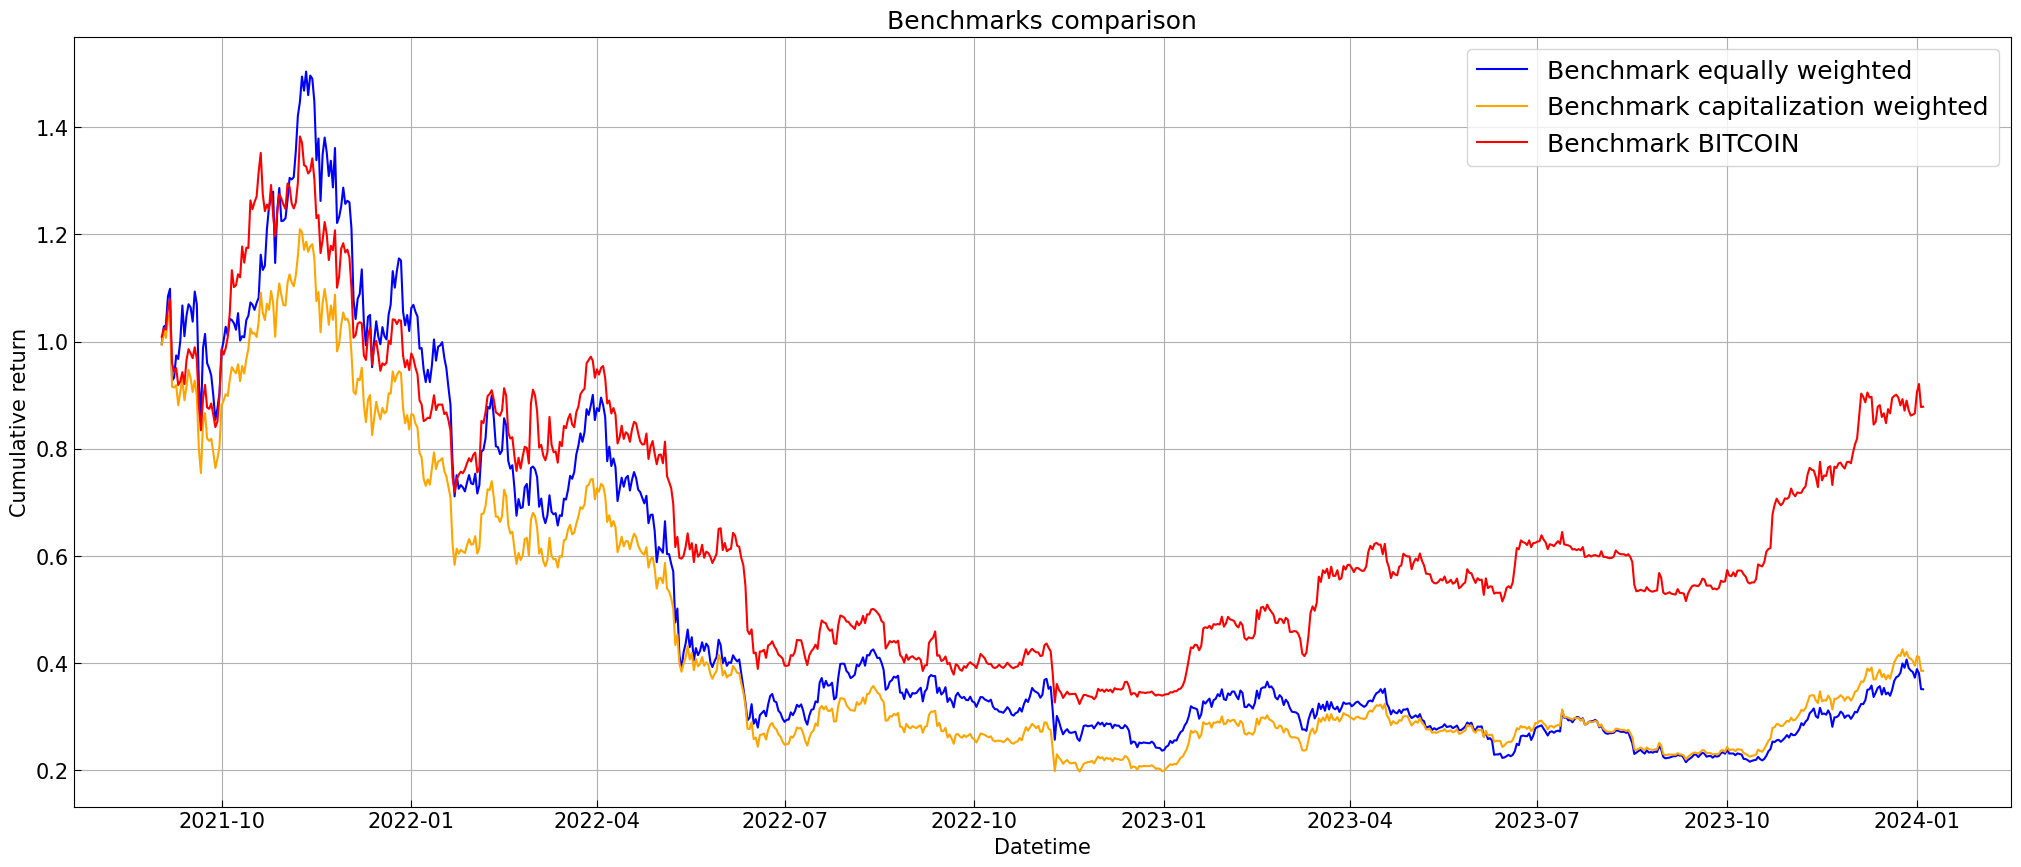
\includegraphics[width=1\linewidth]{benchmarks_only.png}
    \caption{The historical track of the 3 benchmarks used in this paper}
  \label{fig:fig1}
\end{figure}
It clearly appears that the BITCOIN outperform drastically the other benchmarks, this bias will be taken in into account when comparing the performances.
\subsection{Performance and risk metrics}\label{subsec:perfandrisk}
To gauge the effectiveness of various iterations of the momentum strategy, we will employ the following set of performance metrics and risk metrics. All the metrics computed will be presented as annualized in the section \ref{sec:mainres}.


The \textbf{expected return} (\(r_P\)) is a scalar denoting the average gain or loss an investor can anticipate. It is computed as the arithmetic mean of daily strategy returns:
    \[r_P=\mathbb{E}[r_p]=\Bar{r_p}=\frac{1}{N}\sum_{i=1}^Nr_{p_i}\]
    
The historical \textbf{volatility} (\(\sigma_P\)) serves as a risk measure, representing the standard deviation of returns around the mean over a specific period:
    \[\sigma_P = \sqrt{\frac{1}{N-1}\times\sum^N_{i=1}(r_{p_i}-\Bar{r_p})^2}\]

The historical \textbf{value-at-risk (VaR)} is a risk measure denoting the potential loss at a specified percentile of the returns distribution (\(1-\alpha\)):
    \[\text{VaR}_{1-\alpha}(X)=\text{inf}_{t\in\mathbb{R}}\{t:P(X\leq t)\geq1-\alpha\}\]

The historical \textbf{conditional value-at-risk (CVaR)} is the average loss for extreme returns, usually conditioned as lower than the value-at-risk:
    \[\text{CVaR}_{1-\alpha}(X)=\frac{1}{\alpha}\int_\alpha^1\text{VaR}_{1-\gamma}(X)d\gamma\]

The \textbf{beta} (\(\beta\)) represents the sensitivity of a strategy to a benchmark. A beta greater than 1 implies an overreaction to benchmark changes:
    \[\beta = \frac{\text{cov}(r_p,r_b)}{\sigma_B^2}\]

The \textbf{tracking error} (\(\text{TE}\)) measures the average deviation of the strategy from a benchmark, providing an ex-post risk measure:
    \[\text{TE}=\sqrt{\mathbb{V}(r_p-r_b)}\]

The \textbf{Sharpe ratio} (\(\text{SR}\)) is an absolute performance measure, quantifying the excess return from a strategy per unit of volatility:
    \[\text{SR} = \frac{r_P-r_F}{\sigma_P}\]

The \textbf{information ratio} (\(\text{IR}\)) is a relative performance measure for portfolio management, replacing the risk-free rate with the benchmark expected return and using tracking error in the denominator:
    \[\text{IR} = \frac{r_P-r_B}{TE}\]

The \textbf{tail ratio} (\(\text{TR}\)) is a risk measure, representing the ratio of conditional average gain over the inverse conditional loss. A value greater than one indicates an asymmetric strategy with positive extreme returns higher than negative extreme returns:
    \[\text{TR}=\vert\frac{\text{CVaR}_{0.05}(X)}{\text{CVaR}_{0.95}(X)}\vert\]


All these metrics will be detailed in section\ref{sec:mainres}, accompanied by their respective t-statistics. The inclusion of t-statistics is crucial for evaluating the significance of the strategy in comparison to the benchmark. Considering the limited historical data comprising approximately 855 data points, we opted for a statistical bootstrap sampling with replacement approach. This technique involves the random selection of 200 returns from the available 855 data points, repeated 1000 times. With each iteration, we compute the entire suite of metrics, allowing us to conduct a two sided t-test. The hypotheses for the t-test are as follow:
\begin{itemize}
    \item $H_0$ : The strategy computed metric is the equal to the benchmark computed metric
    \item $H_1$ : The strategy computed metric is different from the benchmark computed metric
\end{itemize}

\subsection{Different momentum formula}\label{subsec:momentumformulas}
Momentum in finance denotes the tendency of assets that have demonstrated robust performance, either positively or negatively, in the past, to persist in their price movements in the same direction for a specific period Titman et al. (1993)\cite{Titman1993}. The fundamental premise of momentum investing is grounded in the belief that assets that have recently performed well are likely to continue performing positively, while those that have performed poorly are likely to persist in underperformance Asness et al. (2009)\cite{Asness2009}.
\newline
In practical terms, there exist various methods for quantifying the best and worst performers over a given period. Consequently, this paper aims to distinctly define four approaches for calculating asset momentum to facilitate the backtesting of these different momentum strategies.
\newline
The four distinct momentum formulas are articulated as follows:
\newline\newline
\textbf{Price momentum} : given an asset price time series $\{p_1, p_2, ..., p_n\}$ at each point $i$ the $k$-periods price momentum is computed as : $$\textit{price momentum}^{k}_i = \frac{p_i}{p_{i-k}}$$ \newline

\textbf{Time series momentum} : This formula is directly applied from Moskowitz et al. (2011) \cite{Moskowitz2011}. Given a time series of daily returns $\{r_1, r_2, ..., r_n\}$ and its associated $k$-periods rolling volatility $\{\sigma_1^k, \sigma_2^k, ..., \sigma_n^k\}$ then at each point $i$, the 1 year TSMOM is computed as follow: $$\textit{TSMOM}^{365}_{i}=\text{sign}(r_{i-12})\times\frac{40\text{\%}}{\sigma_i^{365}}\times r_i$$ \newline
\textbf{Moving average momentum} : The moving average momentum is basically the potential return of the price over the its exponential moving average. A high and positive distance indicates a strong momentum. Therefore given an asset prices time series $\{p_1, p_2, ..., p_n\}$ then we compute the exponential moving average over $k$ periods with the following formula : $\textit{EMA}^k_i=\frac{1}{k}\sum_{j=0}^k \alpha\times(1-\alpha)^j\times p_i-j$. Now their is  another time series $\{\text{EMA}_1^k, \text{EMA}_2^k, ..., \text{EMA}_n^k\}$. Then the moving average momentum at each point $i$ is computed as follow: $$\textit{EMAMOM}^k_i=\frac{p_i}{EMA_i^k}$$\newline

\textbf{Volatility-neutral momentum} : The concept of volatility-neutral momentum aligns with price momentum, albeit with an additional consideration for mitigating the impact of noise inherent in price movements. This is achieved by normalizing the volatility effect, wherein the price momentum is divided by the volatility over the same period during which the price momentum is computed. Given a time series of daily returns $\{r_1, r_2, ..., r_n\}$ and its associated $k$-periods rolling volatility $\{\sigma_1^k, \sigma_2^k, ..., \sigma_n^k\}$ then at each point $i$, the volatility-neutralized momentum formula is articulated as follows: $$\textit{vol neutral momentum}^{k}_i = \frac{p_i}{p_{i-k}}\times\frac{1}{\sigma_i^k}$$
Remark : Only the TSMOM is can be negative therefore we will not use it to perform asset allocation.
\subsection{Backtest implementation}\label{subsec:backtestimplem}
Backtesting a strategy is a quantitative methodology used to assess the historical performance of an investment strategy based on past market data. In essence, it involves applying a set of predefined rules or algorithms to historical market data to simulate how the strategy would have performed over a specific time period. The primary goals of backtesting are to evaluate the strategy's effectiveness, understand its historical risk and return characteristics, and gain insights into its potential future performance. Therefore to be relevant backtest must assert that a each iteration the future data points are unknown it has to be an online process.
\newline
In order to backtest an investment strategy we have to define several things. First of all we need to provide a universe. The universe is described in the section \ref{sec:data} and \ref{sec:descstats}. Then we need to specify the asset selection method and asset allocation method. Theses methods represent the strategy's decisions made over time at each rebalance period. At each rebalance date, all the previous securities in the portfolio are sold. Then the new cash is available and ready to be invested in the newly selected securities.

\subsubsection{Asset selection}
To implement the strategy we need to define the asset selection methodology. As we focus on momentum based investment in this research paper, the asset selection will be performed by ranking in descending order the universe's securities by their momentum. The word momentum here refers to the formulas defined in the section \ref{subsec:momentumformulas}. Once the securities are sorted the algorithm select the $k$ best performing cryptocurrencies. $k$ here is a user defined input, also know as hyperparameter of the strategy, like the momentum window, etc.
\subsubsection{Asset allocation}\label{subsubsec:assetalloc}
As the asset selection has been performed, the next step is to allocate a fraction of the cash in the newly selected assets. In this paper we would also like to find the best way to allocate the assets given a momentum calculation. Therefore we used four different asset allocate methods:\newline\newline
\paragraph{Equally weighted allocation} : The equally weighted allocation is the most simple one, the fraction of cash invested in each securities is the same. Therefore the weight for the asset $i$ given $n$ assets in the portfolio is the following: $$w_k=\frac{1}{n}$$
\paragraph{Capitalization weighted allocation} : The capitalization weighted allocation is quite simple the fraction of cash invested in each securities is proportional to the market capitalization of each asset selected. Therefore the weight for the asset $i$ given $n$ assets in the portfolio is the following: $$w_k=\frac{\textit{market cap}_k}{\sum_{j=0}^n\textit{market cap}_j}$$
%\paragraph{Momentum weighted allocation} : momentum weighted allocation is quite simple the fraction of cash invested in each securities is proportional to the momentum of each asset selected. Therefore the weight for the asset $i$ given $n$ assets in the portfolio is the following: $$w_k=\frac{\textit{momentum}_k}{\sum_{j=0}^n\textit{momentum}_j}$$
\paragraph{Mean variance allocation} : The mean variance allocation is a bit more complex than the three previous one. This one in basically a convex optimization problem. Our output is a line vector containing the weight for each asset, this is the vector $w$. Then we need to define the objective function: $$f(w)=\frac{\mathbb{E}[r_P]}{\sigma_P}$$
where:
\begin{itemize}
    \item $\sigma_P=\sqrt{w^T \Sigma w}$ is the volatility of the portfolio
    \item $\mathbb{E}[r_P]=w \cdot R$ is the expected return of the portfolio
    \item $\Sigma$ is the variance-covariance matrix of the $n$ assets returns
    \item $R$ a column vector containing the expected returns for each of the $n$ assets.
\end{itemize}
The optimization problem is to find the weights $w$ that maximize the objective function subject to constraints:
\[
\begin{cases}
\textbf{} & w^*=\text{argmax}(f(w)) \\
 \text{}& \text{s.t.} \quad\sum_{i=1}^{n} w_i = 1 \quad \text{(sum of weights is 1)} \\
 \text{} & \text{s.t.} \quad w_i \geq 0 \quad \text{(long-only portfolio)}
\end{cases}
\]
\newline
\paragraph{Risk parity allocation} : The risk parity allocation Roncalli et al. (2008)\cite{Maillard2008} is a even more complex than the previous one. This one in basically a convex optimization problem. But in this case the aim is to allocate equally the risk contribution of the $n$ asset in the portfolio. A very risky asset will have a lower weight. Our output is a line vector containing the weight for each asset, this is the vector $w$. Then we define the objective function, this is defined as the squared Euclidean norm of the difference between actual risk contributions (\(AC\)) and target risk contributions (\(TRC\)):

$$f(w) = \lVert AC - TRC \rVert^2=\left\lVert \begin{bmatrix} RC_1 \\ RC_2 \\ \vdots \\ RC_n \end{bmatrix} - \begin{bmatrix} \frac{1}{n} \sigma_P \\ \frac{1}{n} \sigma_P \\ \vdots \\ \frac{1}{n} \sigma_P \end{bmatrix} \right\rVert^2$$

where:
\begin{itemize}
    \item $RC_k = \frac{\partial \sigma_P}{\partial w_k}$ is the risk contribution of each asset
    \item $\sigma_P=\sqrt{w^T \Sigma w}$ is the volatility of the portfolio
    \item $\Sigma$ is the variance-covariance matrix of the $n$ assets returns
\end{itemize}

The optimization problem is to find the weights $w$ that maximize the objective function subject to constraints:

\[
\begin{cases}
\text{} & w^*=\text{argmax}\{\lVert AC - TRC \rVert^2\} \\
\text{} & \text{s.t.}\quad \sum_{i=1}^{n} w_i = 1 \quad \text{(sum of weights is 1)} \\
\text{} & \text{s.t.}\quad w_i \geq 0 \quad \text{(long-only portfolio)}
\end{cases}
\]

Allocation adjustments are executed at each rebalance date, occurring at periodic intervals such as weekly, monthly, or quarterly occurrences. Notably, the backtesting procedure must consider the phenomenon of weight drift. As the portfolio's assets evolve on a daily basis, ensuring that the sum of weights remains constant at 1, the weights undergo daily adjustments. The weight drift is mathematically expressed by the following formula:
 
$$w_{k,i}=\frac{w_{k,i-1} (1+r_{k,i})}{\sum_{j=1}^n w_{j,i-1}(1+r_{j,i})}$$
Where $k$ is the asset index and $i$ is the time index.\newline
In each iteration of the backtest implementation, the following formula is employed to enhance the realism of the simulation.
\subsubsection{Transaction costs and slippage effect}
To enhance the realism of our backtesting process, we incorporate transaction costs at each rebalance date, reflecting the expenses incurred in selling all existing securities and acquiring new ones. Given that our asset universe comprises cryptocurrencies, we implement transaction costs based on those observed on the Binance exchange, a prominent platform in this domain. Specifically, for both buying and selling a security, a transaction cost of 0.1\% of the nominal value is applied. Only market orders are supposed to be executed, thereby incurring taker fees.\newline\newline
Additionally, the execution of market orders exposes us to the slippage effect, denoting the marginal difference between the intended transaction price and the actual executed price. Such disparities may arise due to bid-ask spreads or liquidity constraints. We posit that the slippage effect consistently amounts to 0.05\% per transaction.

\section{Descriptive statistics}\label{sec:descstats}

\paragraph{}
We systematically collected daily data covering the period from 2 September 2021 to 4 January 2024, constituting a sample of 855 data points. The information collected includes key fields such as price, market capitalisation and volume.
Specifically for this section, we have limited ourselves to the price of each asset in order to carry out an individual descriptive analysis by asset.
Firstly, we calculate the logarithmic return for each asset, and then we calculate the mean, median, min, max, kurtosis coefficient and skewness coefficient for these returns (to measure the concentration of values close to the mean in relation to a normal distribution and the asymmetry of the distribution in relation to the mean, respectively) and we summarise this in table 1 below.

%\begin{landscape}
\begin{table}[H]
  \centering
  \begin{tabular}{p{3cm}|p{1.5cm}|p{1.5cm}|p{1.5cm}|p{1.5cm}|p{1.5cm}|p{1.5cm}|p{1.5cm}|p{1.5cm}}%|p{1.60cm}}%{lllllllllll}
    \toprule
    Annual log returns & Mean & Median & Max & Min & Std dev & Kurtosis & Skewness & t-stat \\%& \% return > 0 \\
    \midrule
    DOGE-USDT & -0.00105 & 0.00013 & 0.37 & -0.23 & 0.047236 & 8.73 & 0.587 & -0.664 \\
    BNB-USDT  & -0.00013 & 0.0003 & 0.130 & -0.204 & 0.034127 & 4.65 & -0.647 & -0.111 \\ 
    XRP-USDT &  -0.0003 & 0.00037 & 0.55 & -0.208 & 0.0447 & 28.64 & 2.13 & -0.20 \\
    ETH-USDT &  -0.00014 & -0.00018 & 0.166 & -0.200 & 0.038 & 3.42 & -0.35 & -0.111 \\  
    VET-USDT &  -0.0012 & 0.0006 & 0.162 & -0.242 & 0.046 & 2.30 & -0.35 & -0.779 \\  
    AVAX-USDT & 0.00105 & 0.00062 & 0.246 & -0.356 & 0.058 & 3.80 & -0.06 & 0.538 \\
    MATIC-USDT & -0.00025 & -0.00011 & 0.32 & -0.274 & 0.054 & 4.21 & 0.23 & -0.135 \\  
    SOL-USDT  & 0.00112 & -0.0012 & 0.28 & -0.547 & 0.058 & 9.85 & -0.63 & 0.566 \\  
    BTC-USDT  & 0.00015 & -0.00039 & 0.135 & -0.167 & 0.03 & 4.014 & -0.38 & 0.150 \\ 
    BCH-USDT & -0.00092 & -0.00058 & 0.310 & -0.184 & 0.042 & 6.24 & 0.51 & -0.639 \\  
    LTC-USDT & -0.00085 & 0.00082 & 0.249 & -0.208 & 0.043 & 3.99 & -0.25 & -0.592 \\  
    ADA-USDT & -0.00111 & -0.001 & 0.210 & -0.206 & 0.044 & 2.96 & 0.17 & -0.752 \\  
    DASH-USDT & -0.0011 & 0.0028 & 0.144 & -0.255 & 0.045 & 3.10 & -0.78 & -1.289 \\ 
    EOS-USDT & -0.0012 & -0.00010 & 0.177 & -0.250 & 0.044 & 3.90 & -0.79 & -1.298 \\  
    LINK-USDT &  -0.00051 & 0.0023 & 0.190 & -0.214 & 0.048 & 2.00 & -0.37 & -0.366 \\  
    XLM-USDT  & -0.001 & 0.00010 & 0.478 & -0.234 & 0.042 & 20.88 & 1.30 & -0.707 \\  
    ATOM-USDT & -0.00031 & 0.0015 & 0.266 & -0.265 & 0.054 & 3.64 & 0.14 & -0.166 \\ 
    ETC-USDT  & -0.0010 & -0.0015 & 0.271 & -0.218 & 0.047 & 5.08 & 0.44 & -0.624 \\  
    KDA-USDT  & 0.0013 & -0.0022 & 0.412 & -0.337 & 0.069 & 5.00 & 0.76 & 0.559\\  
    TRX-USDT &  0.0005 & 0.0022 & 0.172 & -0.195 & 0.033 & 7.12 & -0.48 & 0.440 \\   
    XTZ-USDT & -0.0014 & 0.0017 & 0.309 & -0.240 & 0.050 & 4.85 & 0.083 & -0.841\\

 \bottomrule
\end{tabular}
  \label{tab:volneutmom172meanvar}
   \caption{Log Return Summary Statistics by asset}
\end{table}
%\end{landscape}





\section{Main results}\label{sec:mainres}
\subsection{Optimal momentum and re-balance period}
\subsubsection{Objectives}
\paragraph{}
There are two periods that needs to be optimized: the period used to compute our signal and calculate our allocation that we defined as the lookback period and the period before we need to calculate a new allocation which is called the horizon. 

\paragraph{}
In the next sections, we'll explain how we determined these timeframes. Before we dive in, it's important to note that while optimizing these periods is crucial, there's a risk of overfitting. To address this, we took care to test the reliability of our approach and kept things simple to avoid overfitting issues.

\subsubsection{Presentation of the framework for a given horizon}
\paragraph{}
To illustrate the framework we utilized, let's consider a straightforward example. Our aim is to identify the ideal lookback period for a specific holding horizon of 30 days. In simpler terms, we are seeking the most effective timeframe for assessing data when considering a 30-day investment horizon.

\paragraph{}
Momentum strategies hinge on the persistent nature of returns. In light of this, we have devised a metric to evaluate the continuity of returns within our specified lookback period and subsequent horizon. To quantify this, we introduce two returns series, namely the rolling averages of past returns (\(\text{{lookback}}_{\alpha}\)) and future returns (\(\text{{horizon}}_{\beta}\)):

\[
\text{{lookback}}_{\alpha}(x) = \frac{1}{\alpha} \sum_{i=1}^{\alpha} x_{t-i+1}
\]

\[
\text{{horizon}}_{\beta}(x) = \frac{1}{\beta} \sum_{i=1}^{\beta} x_{t-i+1}
\]

Here:
\begin{itemize}
    \item \(\alpha\) represents the lookback period,
    \item \(\beta\) represents the horizon period,
    \item \(x\) signifies returns.
\end{itemize}

\paragraph{}
Following the computation of these two series, we assess the persistence of returns from the lookback period to the horizon by calculating the correlation coefficient between them. This correlation analysis serves as a valuable indicator of the degree to which past returns align with future returns within the specified timeframes.

\paragraph{}
Our investment universe encompasses a diverse set of assets. To derive comprehensive insights, we apply the aforementioned method to each individual asset, calculating the correlation coefficient. By averaging these coefficients across all assets, we obtain a generalized result. The ensuing graph visually represents the collective outcomes:

\begin{figure}[H] % picture
    \centering
    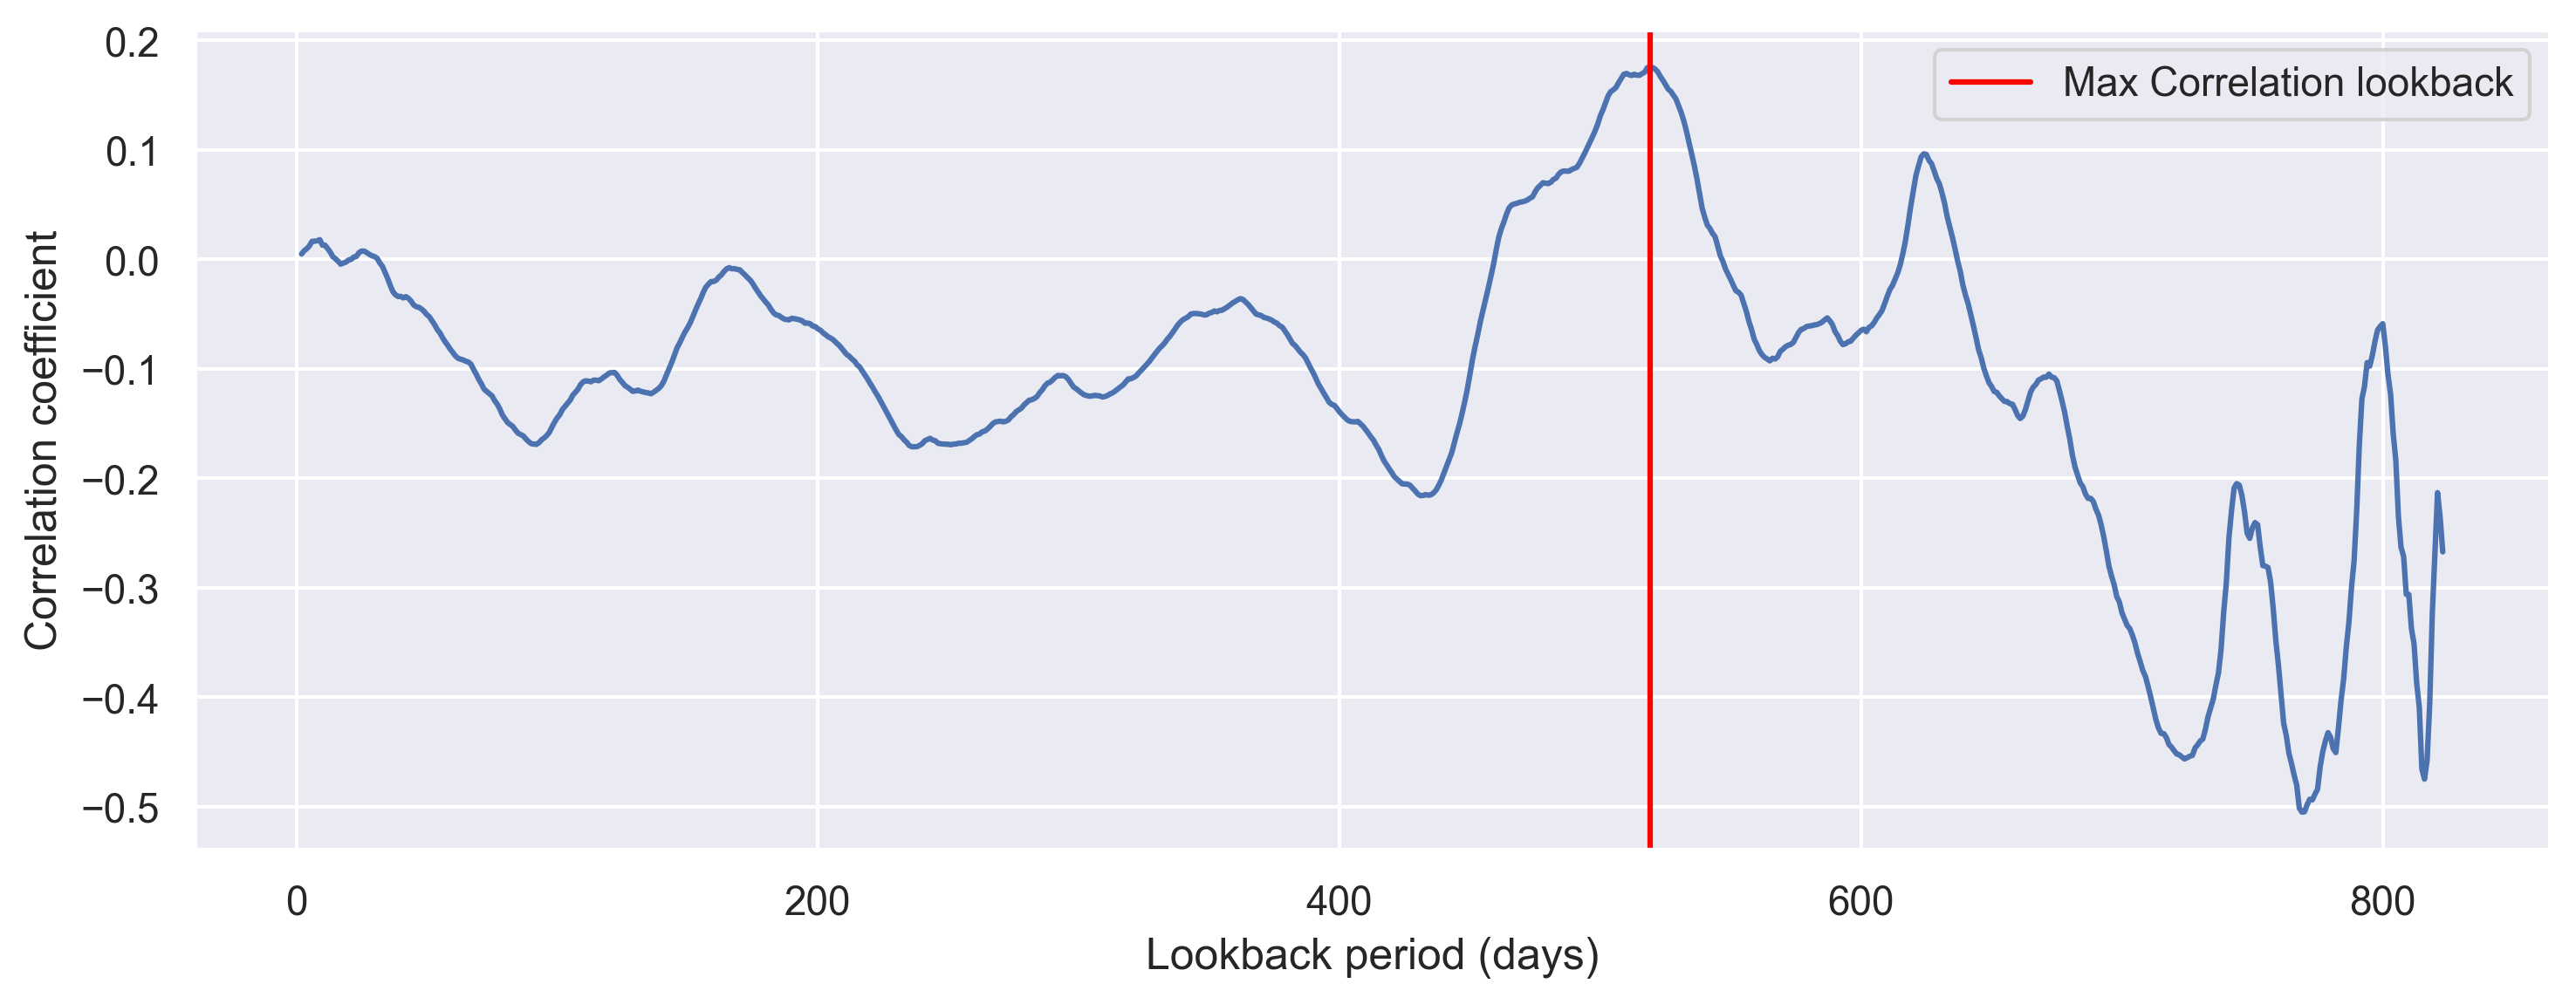
\includegraphics[width=1\linewidth]{fixed_window.png}
    \caption{Average future returns correlation to average past returns with an horizon of 30 days.}
  \label{fig:fig2}
\end{figure}

\paragraph{}
It becomes evident that distinct lookback periods lead to diverse outcomes. A correlation coefficient below 0 indicates a trend toward mean reversion, while a positive correlation coefficient signifies the presence of momentum. Notably, the maximum correlation coefficient is achieved with a 30-day horizon and a 519-day lookback period. Our subsequent focus involves identifying the optimal combination of lookback and horizon windows.

\subsubsection{Optimal combination of lookback and horizon windows} \label{subsec:opt}
\paragraph{}
We applied the methodology outlined in the preceding subsection to compute correlation coefficients for various lookback and horizon windows. The results are visually represented in the following figure:

\begin{figure}[H] % picture
    \centering
    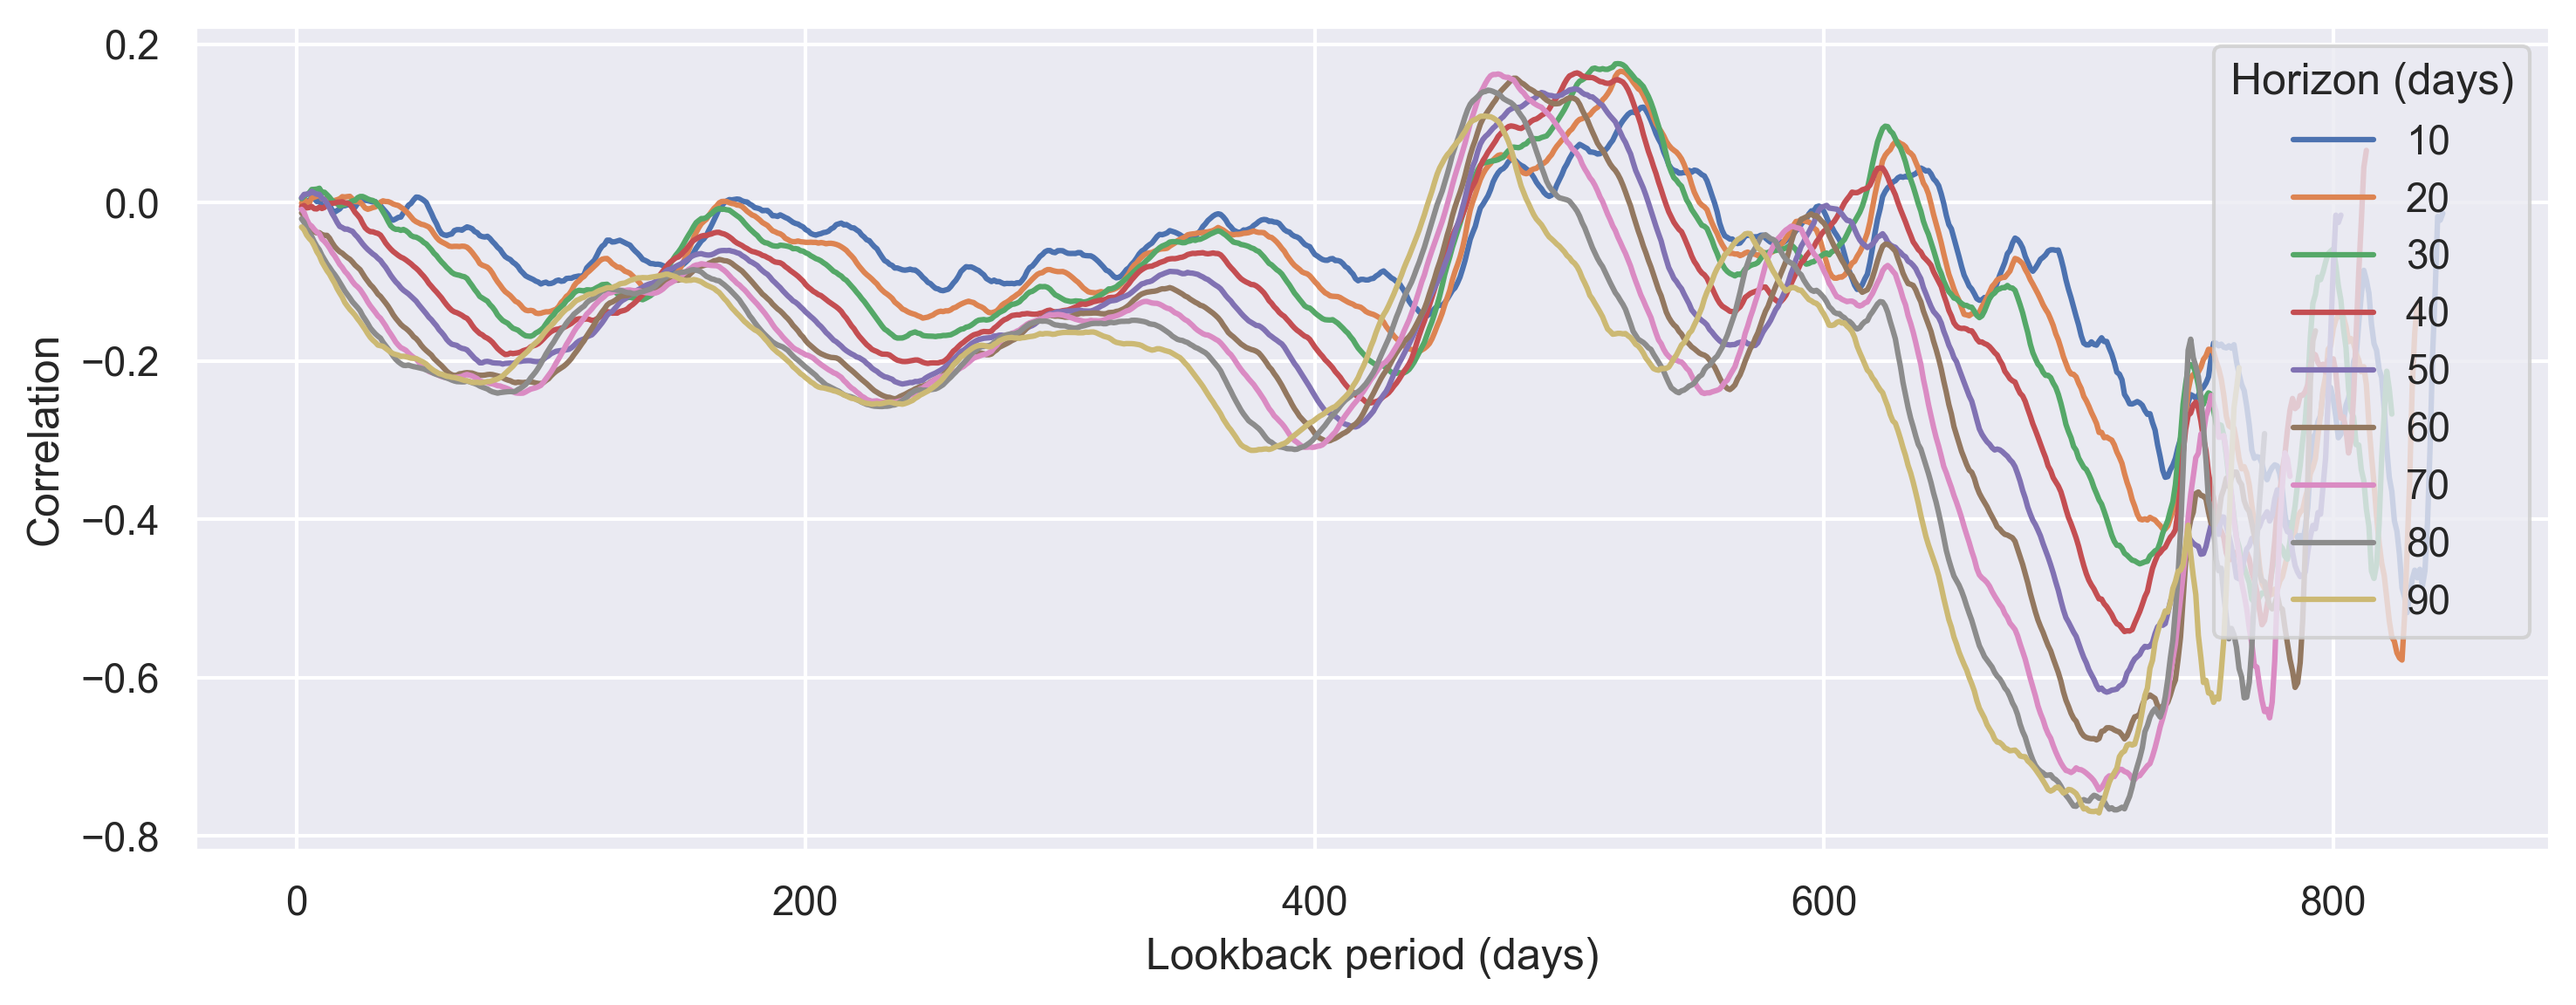
\includegraphics[width=1\linewidth]{combinations.png}
    \caption{Average correlation of future returns to past returns across all horizons.}
    \label{fig:fig3}
\end{figure}

The correlation reaches its maximum when selecting a lookback period of 519 days and a holding horizon of 30 days. This suggests that with this specific combination of parameters, the momentum effect can be exploited to its fullest potential. However, given the limited availability of data, we assess the optimal allocation methods on a lookback period of 365 days. It is important to note that while testing on this shorter period, the optimal allocation lookback we estimated remains at 519 days.


\subsection{Optimal momentum formula, selection \& allocation}\label{subsec:optimomFSA}
The section \ref{subsec:opt} is due to find the most effective window for calculating the momentum. We shall use the 512 periods momentum in this part. However given our history is limited to 832 periods we will take the highest correlated momentum over a one year period. Then a window of 172 is used to calculate all the momentum in the \ref{subsec:momentumformulas}. In this new section given the most effective number of period for computing the momentum we focused on finding an efficient way to allocate the asset's weights in the portfolio. We computed the backtest for each type of momentum calculation. Thus we used the backtest from the section \ref{subsec:backtestimplem} that given a universe, a rebalance period, an asset selection process and an asset allocation process will iterate over each date run the strategy and calculate the performances of this strategy.\newline\newline
We collected the results by varying the number of assets selected among the 21 assets in the universe we considered. This number of assets is later denoted as $k \in\{3, 5, 8, 10, 15\}$.\newline We also varied the benchmarks used to compare our strategies in order to take into account different type of investor. The benchmarks from the section \ref{subsec:bench} where used against each strategy.\newline
The backtest procedure varied the allocation methods used as well. The allocation methods are presented in the section \ref{subsubsec:assetalloc}.
A table of the results for the mean variance allocation and the volatility neutralized momentum formula is presented in the table \ref{tab:volneutmom172meanvar}. All the other results are presented in the section \ref{sec:appendix}. The results are presented in the following format : $\text{value}\quad(\text{t-stats})$. The t-stats were computed using a statistic bootstrap described in the section \ref{subsec:perfandrisk}.
\begin{landscape}
\begin{table}[H]
  \centering
  \begin{tabular}{p{0.4cm}|p{3cm}|p{1.65cm}|p{1.65cm}|p{1.65cm}|p{1.65cm}|p{1.65cm}|p{1.65cm}|p{1.65cm}|p{1.65cm}|p{1.65cm}}%{lllllllllll}
    \toprule
    \multicolumn{2}{c}{Assets \& Benchmarks}                   \\
    \cmidrule(r){1-2}
    $k$ & benchmark & CVaR & Expected return & Expected volatility&Information ratio&Portfolio beta&Sharpe ratio&Tail ratio&Tracking error&VaR\\
    \midrule
    3 & BITCOIN & -10.64\% (-19.05) & 16.06\% (-2.09) & 95.69\% (16.56) & -0.12 (-4.22) &	1.10 (4.67) & 0.17 (-4.04)& 1.19 (1.74)& 74.36\% (32.28)& -6.50\% (-17.65) \\
   3&CAPITALIZATION WEIGHTED&-10.64\% (-9.31)&16.06\% (1.42)&95.69\% (12.32)&0.34 (0.25)&1.14 (5.72)&0.17 (0.50)&1.19 (5.76)&64.65\% (27.95)&-6.50\% (-8.62)
\\ 
3&EQUAL WEIGHTED&-10.64\% (-7.16)&16.06\% (2.09)&95.69\% (10.70)&0.54 (1.98)&1.05 (1.91)&0.17 (1.75)&1.19 (7.25)&62.72\% (31.80)&-6.50\% (-1.71)
\\ 
5&BITCOIN&-9.52\% (-12.76)&27.55\% (1.06)&82.10\% (24.58)&0.05 (0.40)&1.10 (6.57)&0.34 (0.14)&1.11 (3.40)&56.21\% (69.05)&-6.30\% (-15.83)
\\ 
5&CAPITALIZATION WEIGHTED&-9.52\% (-8.24)&27.55\% (1.92)&82.10\% (16.04)&0.71 (1.95)&1.08 (6.22)&0.34 (1.80)&1.11 (5.41)&47.24\% (62.93)&-6.30\% (-7.90)
\\ 
5&EQUAL WEIGHTED&-9.52\% (-1.00)&27.55\% (4.27)&82.10\% (11.15)&0.96 (7.80)&0.98 (-2.19)&0.34 (4.37)&1.11 (8.47)&47.19\% (65.80)&-6.30\% (1.17)
\\ 
8&BITCOIN&-8.93\% (-10.33)&5.49\% (-0.75)&76.70\% (21.47)&-0.40 (-1.32)&1.09 (6.73)&0.07 (-1.57)&1.08 (2.65)&48.16\% (69.87)&-6.09\% (-16.25)
\\ 
8&CAPITALIZATION WEIGHTED&-8.93\% (-6.07)&5.49\% (1.09)&76.70\% (18.49)&0.30 (2.31)&1.06 (10.81)&0.07 (1.01)&1.08 (6.38)&38.51\% (88.94)&-6.09\% (-8.72)
\\ 
8&EQUAL WEIGHTED&-8.93\% (2.89)&5.49\% (1.42)&76.70\% (5.54)&0.60 (2.44)&0.97 (-6.92)&0.07 (1.46)&1.08 (8.35)&38.39\% (82.74)&-6.09\% (7.24)
\\ 
10&BITCOIN&-9.17\% (-11.22)&-5.67\% (-1.82)&77.55\% (21.48)&-0.64 (-4.64)&1.12 (8.52)&-0.07 (-2.75)&1.06 (2.36)&48.21\% (79.53)&-6.32\% (-17.36)
\\ 
10&CAPITALIZATION WEIGHTED&-9.17\% (-6.33)&-5.67\% (-0.35)&77.55\% (15.00)&0.01 (-0.31)&1.08 (8.46)&-0.07 (-0.26)&1.06 (4.55)&38.43\% (79.58)&-6.32\% (-8.60)
\\ 
10&EQUAL WEIGHTED&-9.17\% (1.11)&-5.67\% (1.28)&77.55\% (9.37)&0.31 (2.70)&0.98 (-2.41)&-0.07 (1.17)&1.06 (7.95)&38.11\% (74.98)&-6.32\% (0.80)
\\ 
15&BITCOIN&-9.53\% (-14.33)&18.66\% (-2.69)&82.68\% (31.29)&-0.11 (-2.92)&1.12 (7.94)&0.23 (-3.94)&1.13 (3.98)&55.65\% (83.26)&-6.76\% (-22.02)
\\ 
15&CAPITALIZATION WEIGHTED&-9.53\% (-7.07)&18.66\% (1.68)&82.68\% (20.20)&0.53 (2.47)&1.09 (10.86)&0.23 (1.56)&1.13 (8.30)&46.92\% (70.04)&-6.76\% (-10.62)
\\ 
15&EQUAL WEIGHTED&-9.53\% (-3.46)&18.66\% (1.94)&82.68\% (16.01)&0.80 (5.09)&1.01 (0.92)&0.23 (2.35)&1.13 (10.29)&45.38\% (93.97)&-6.76\% (-2.22)\\
    \bottomrule
  \end{tabular}
  \label{tab:volneutmom172meanvar}
   \caption{Performance \& risks from the backtest for the 172 periods Volatility Neutral Momentum. The underlying strategy is rebalanced monthly.}
\end{table}
\end{landscape}
Given the plethora of portfolio management styles and diverse portfolio managers, we intend to present the results from two distinct perspectives. The primary axis will focus on absolute performance, catering to an absolute portfolio management framework. Conversely, the secondary axis will delve into relative performance, aligning with relative portfolio management concerning a designated benchmark.

\subsubsection{Absolute portfolio management style}\label{subsubsec:absPtfMngt}
In this section we present the result obtained from the backtests in order to conclude on the potential value in using momentum for asset selection. This section will focus on the absolute portfolio management framework. The most important metric to consider in this section is the Sharpe ratio as it is an absolute risk adjusted measure that quantify the return by risk unit. Here the risk is measured with the volatility. We only consider one benchmarks the BITCOIN. However all the results are presents in the appendix section \ref{sec:appendix}. We display the sharpe ratio for each momentum formula.

\begin{figure}[H] % picture
    \centering
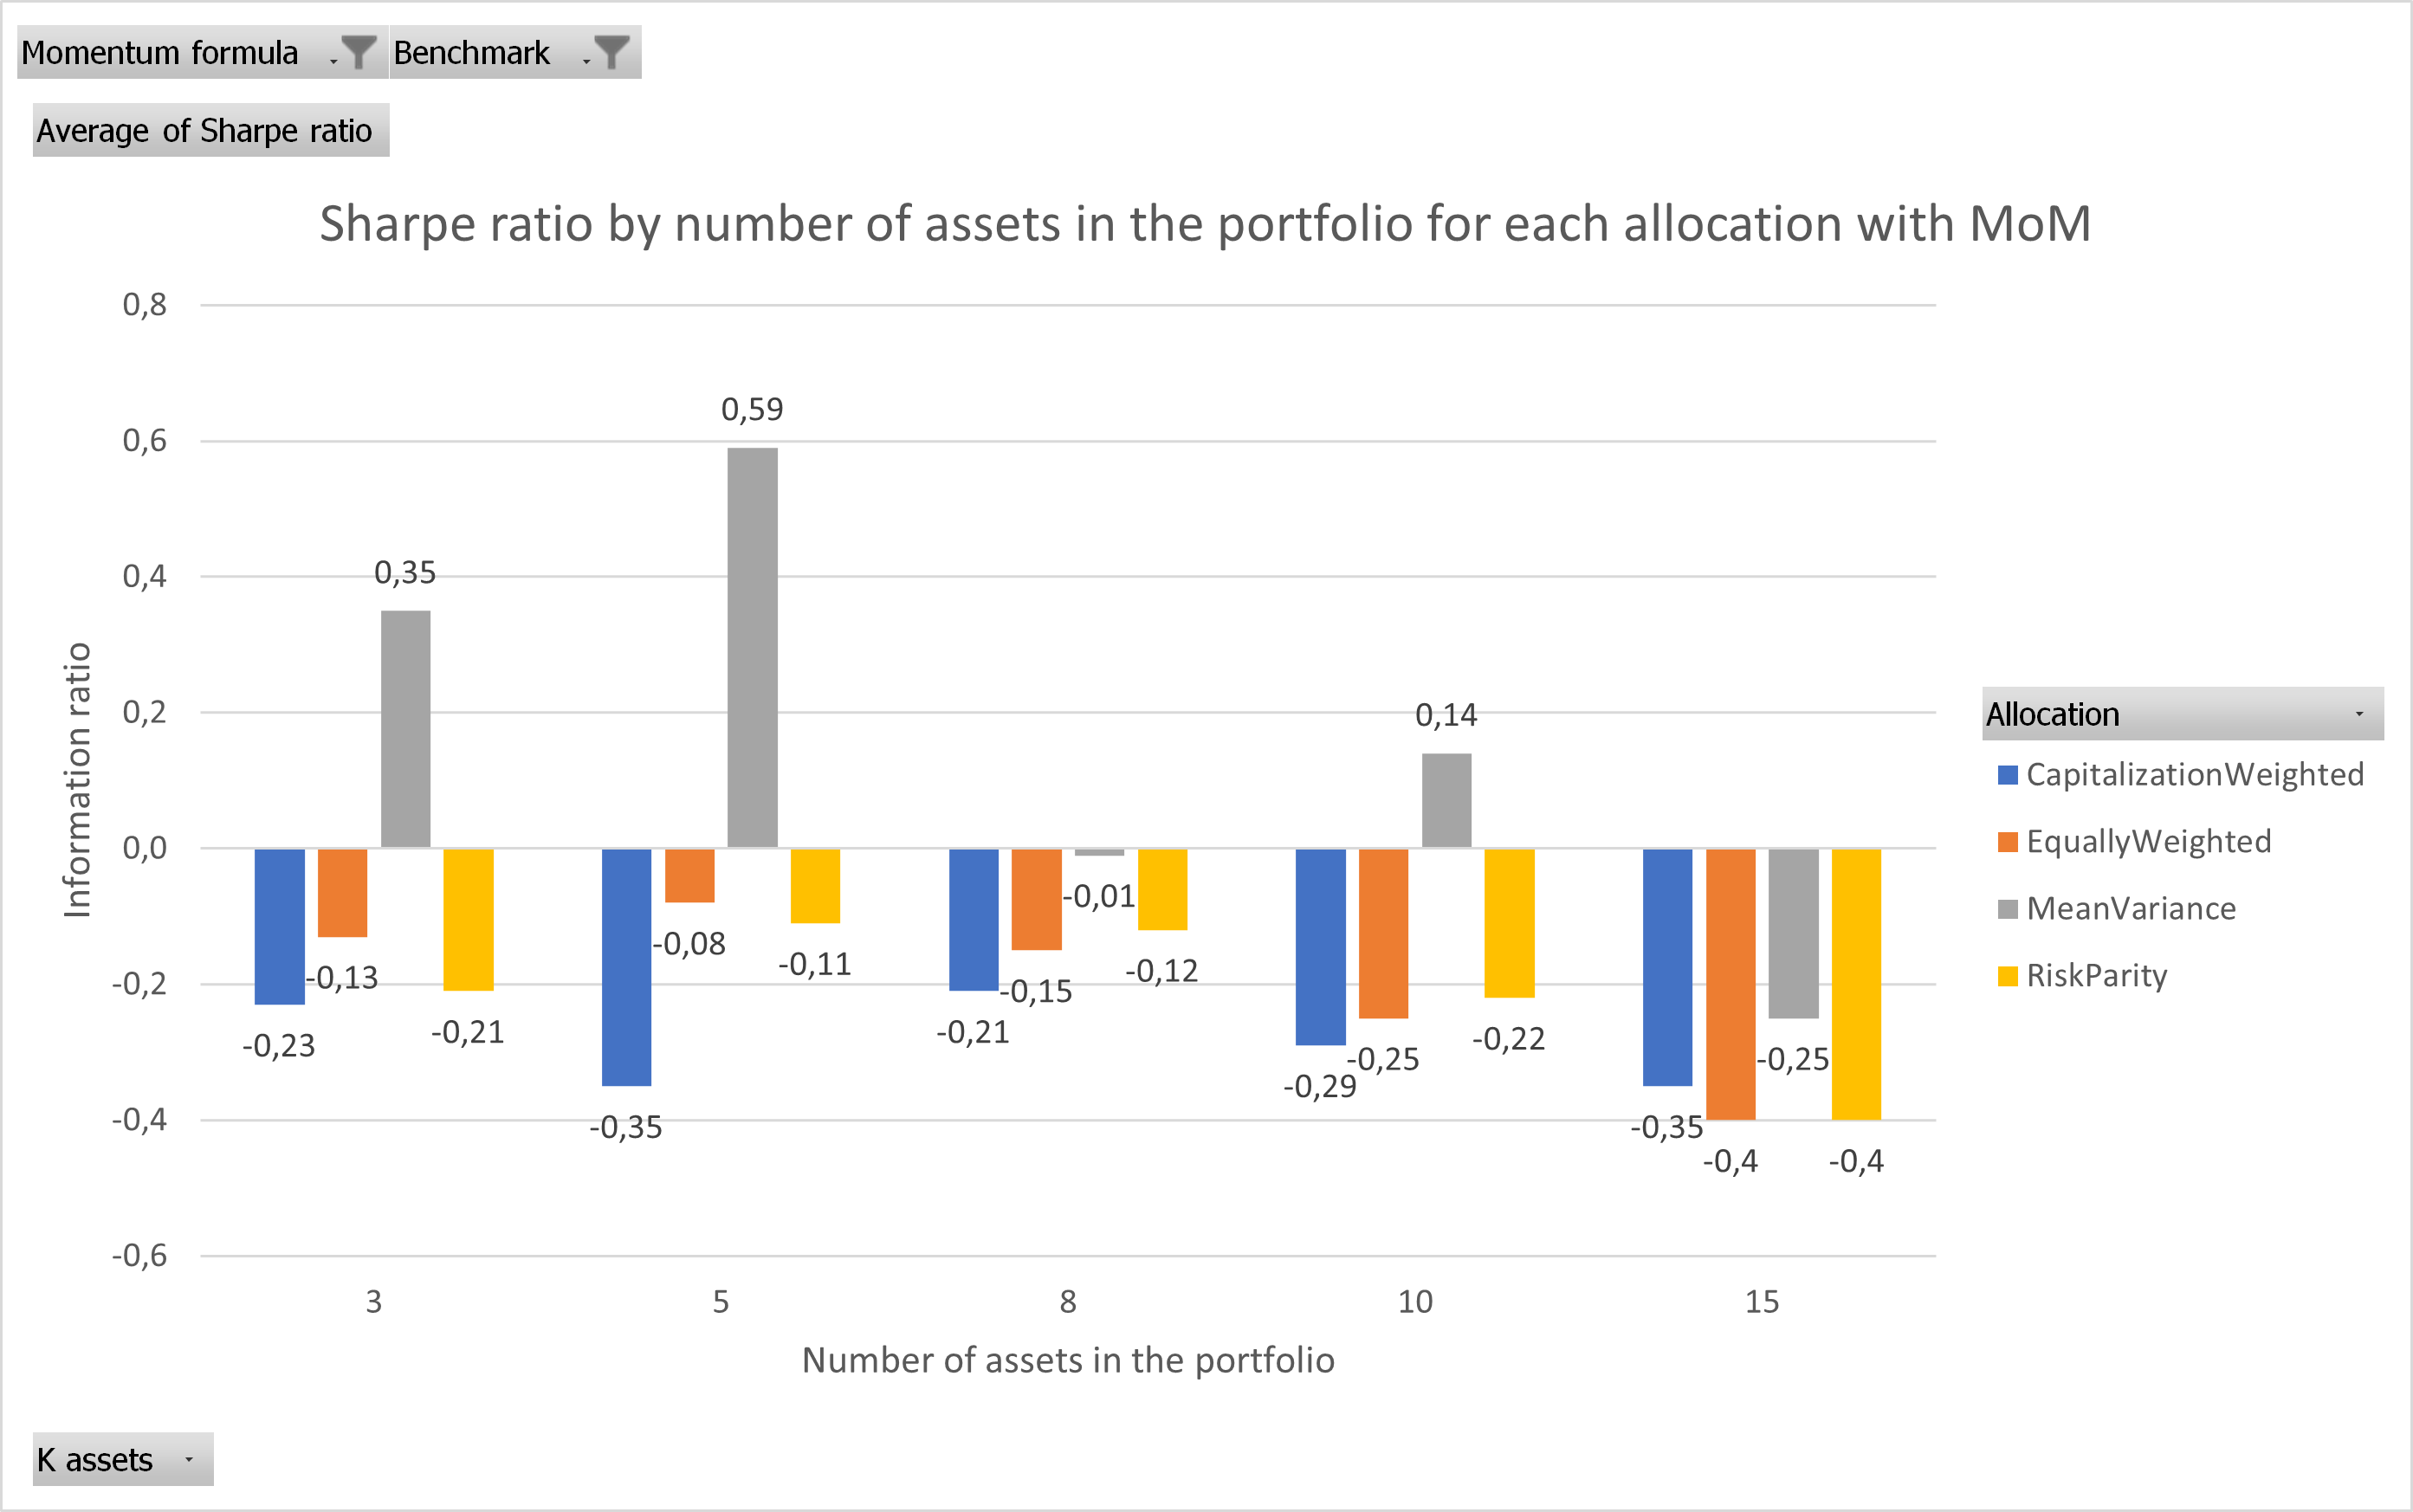
\includegraphics[width=0.75\linewidth]{absolute_management/Sharpe ratio MoM.png}
    \caption{Average Sharpe ratio for each asset allocation method with respect to the number of assets selected in the portfolio for the Price Momentum formula}
    \label{fig:Sharpe ratio MoM}
\end{figure}

\begin{figure}[H] % picture
    \centering
    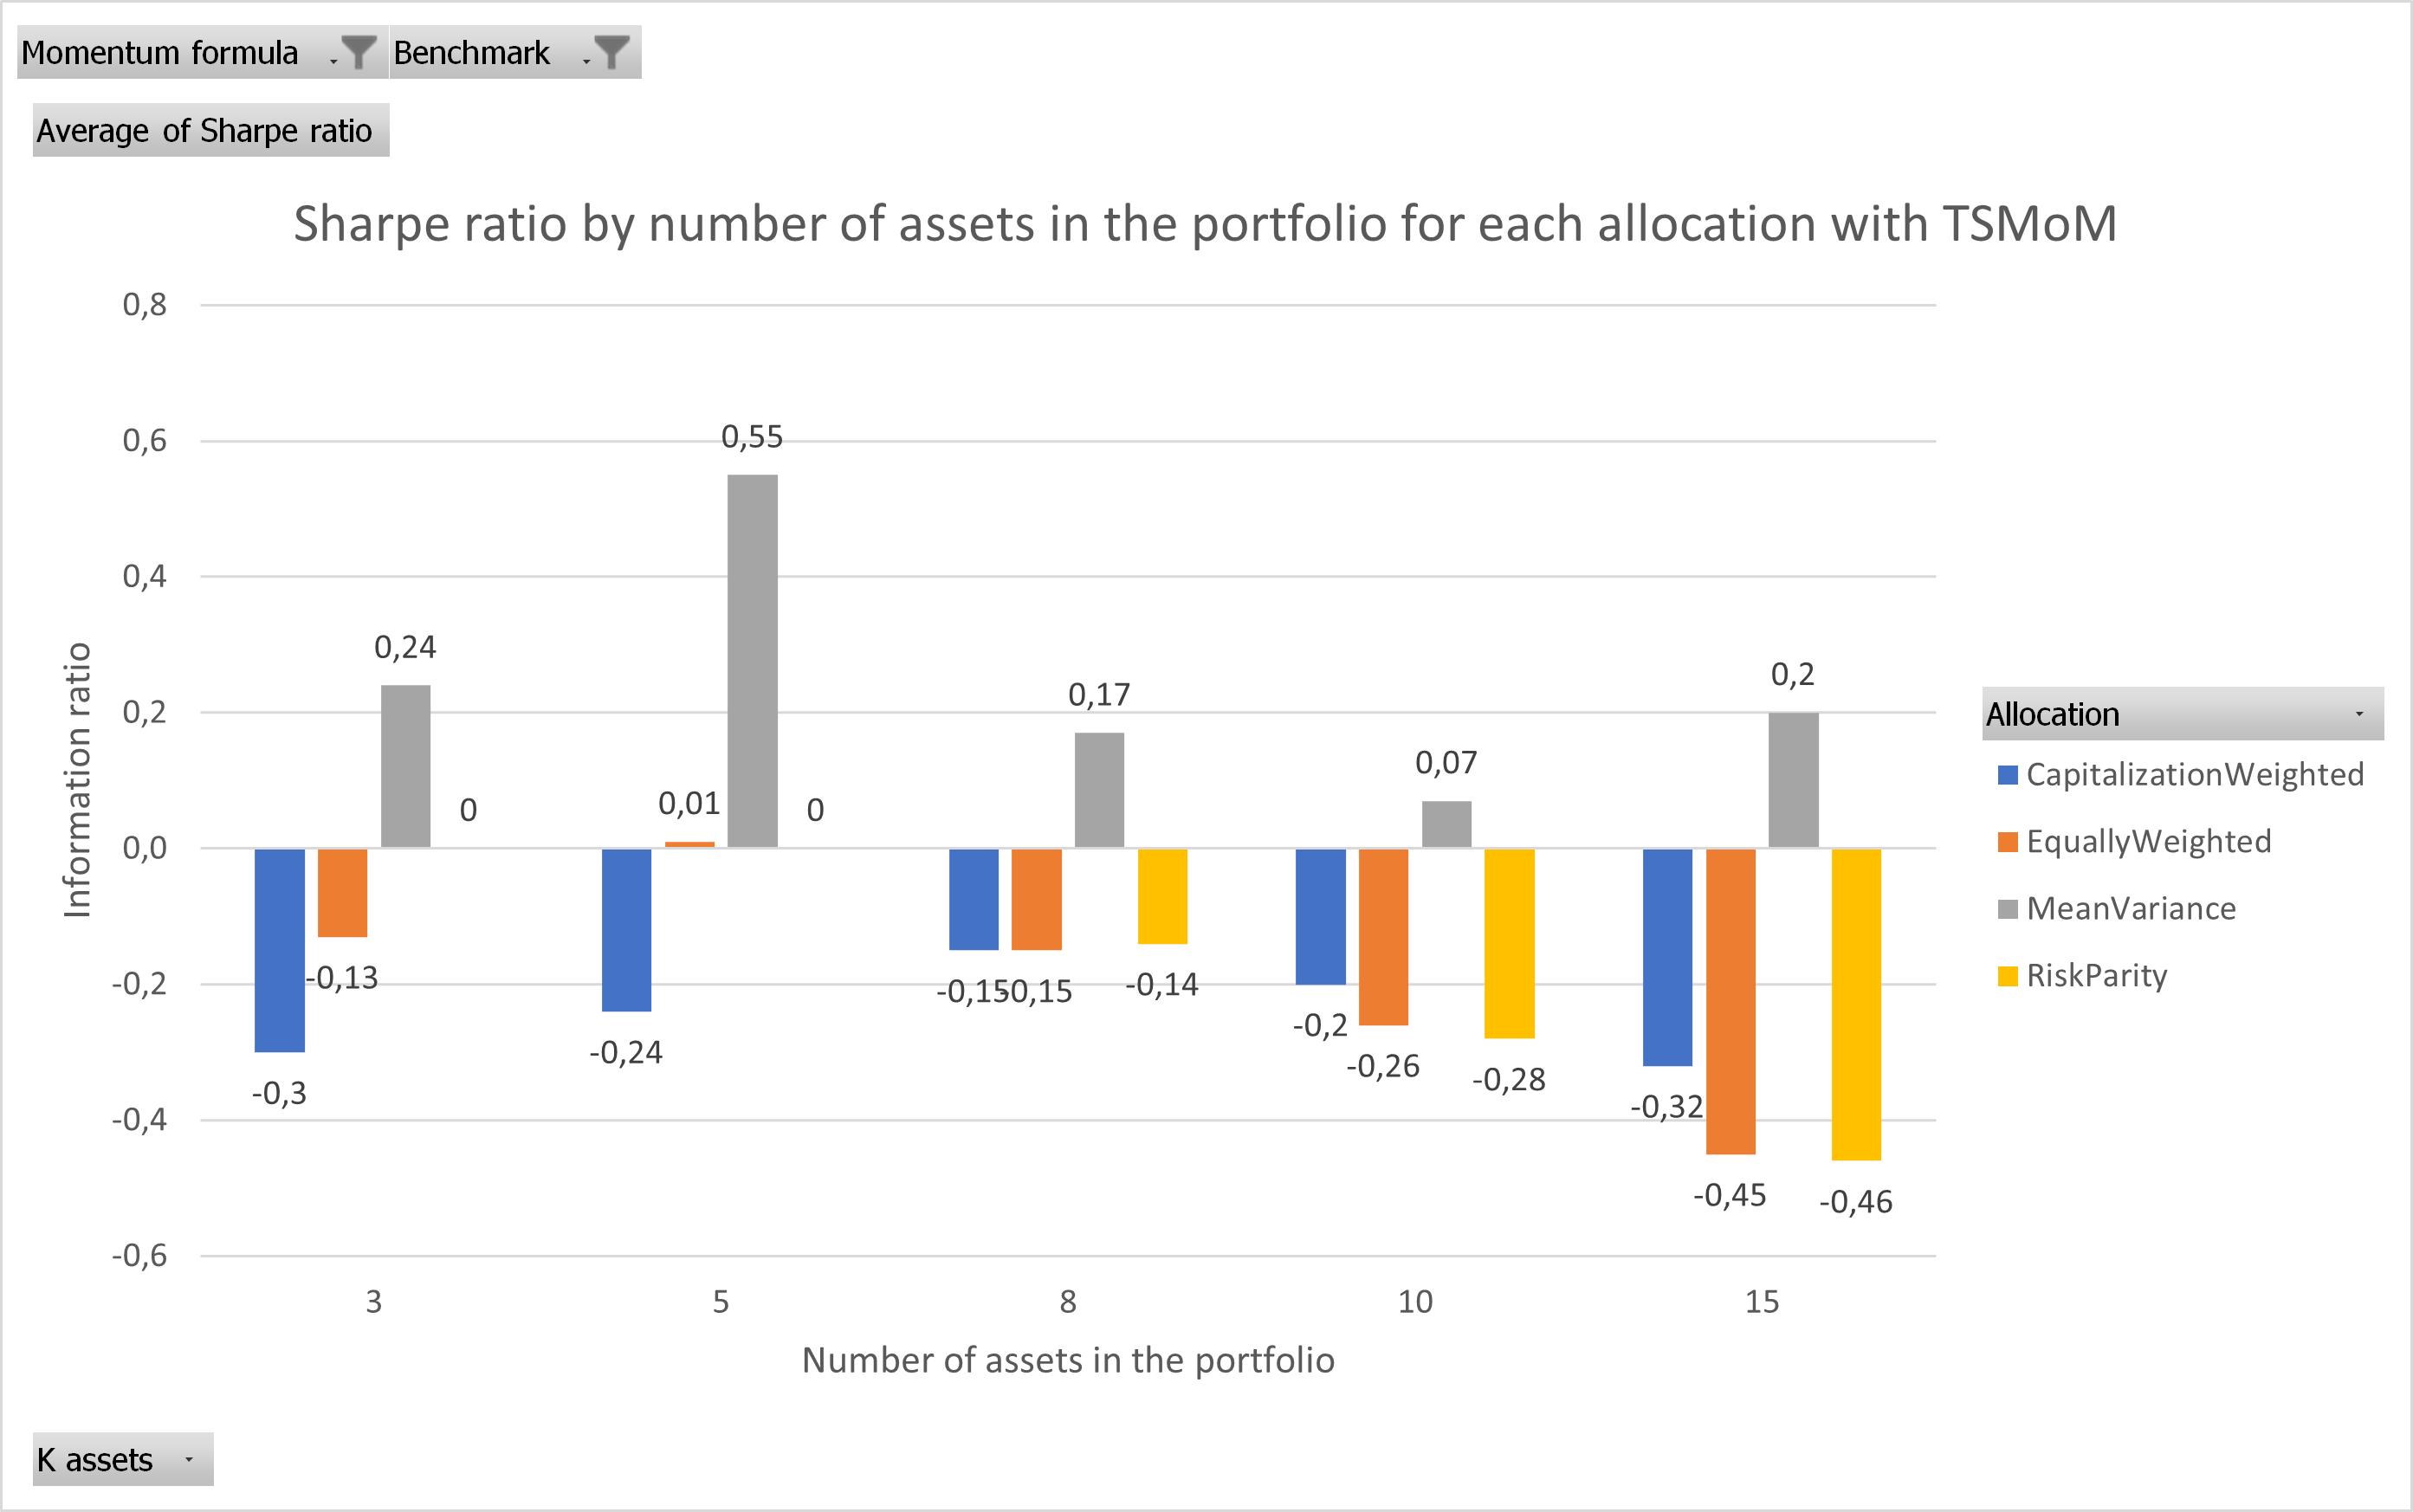
\includegraphics[width=0.75\linewidth]{absolute_management/Sharpe ratio TSMoM.png}
    \caption{Average Sharpe ratio for each asset allocation method with respect to the number of assets selected in the portfolio for the Time Series Momentum formula}
    \label{fig:Sharpe ratio TSMOM}
\end{figure}

\begin{figure}[H] % picture
    \centering
    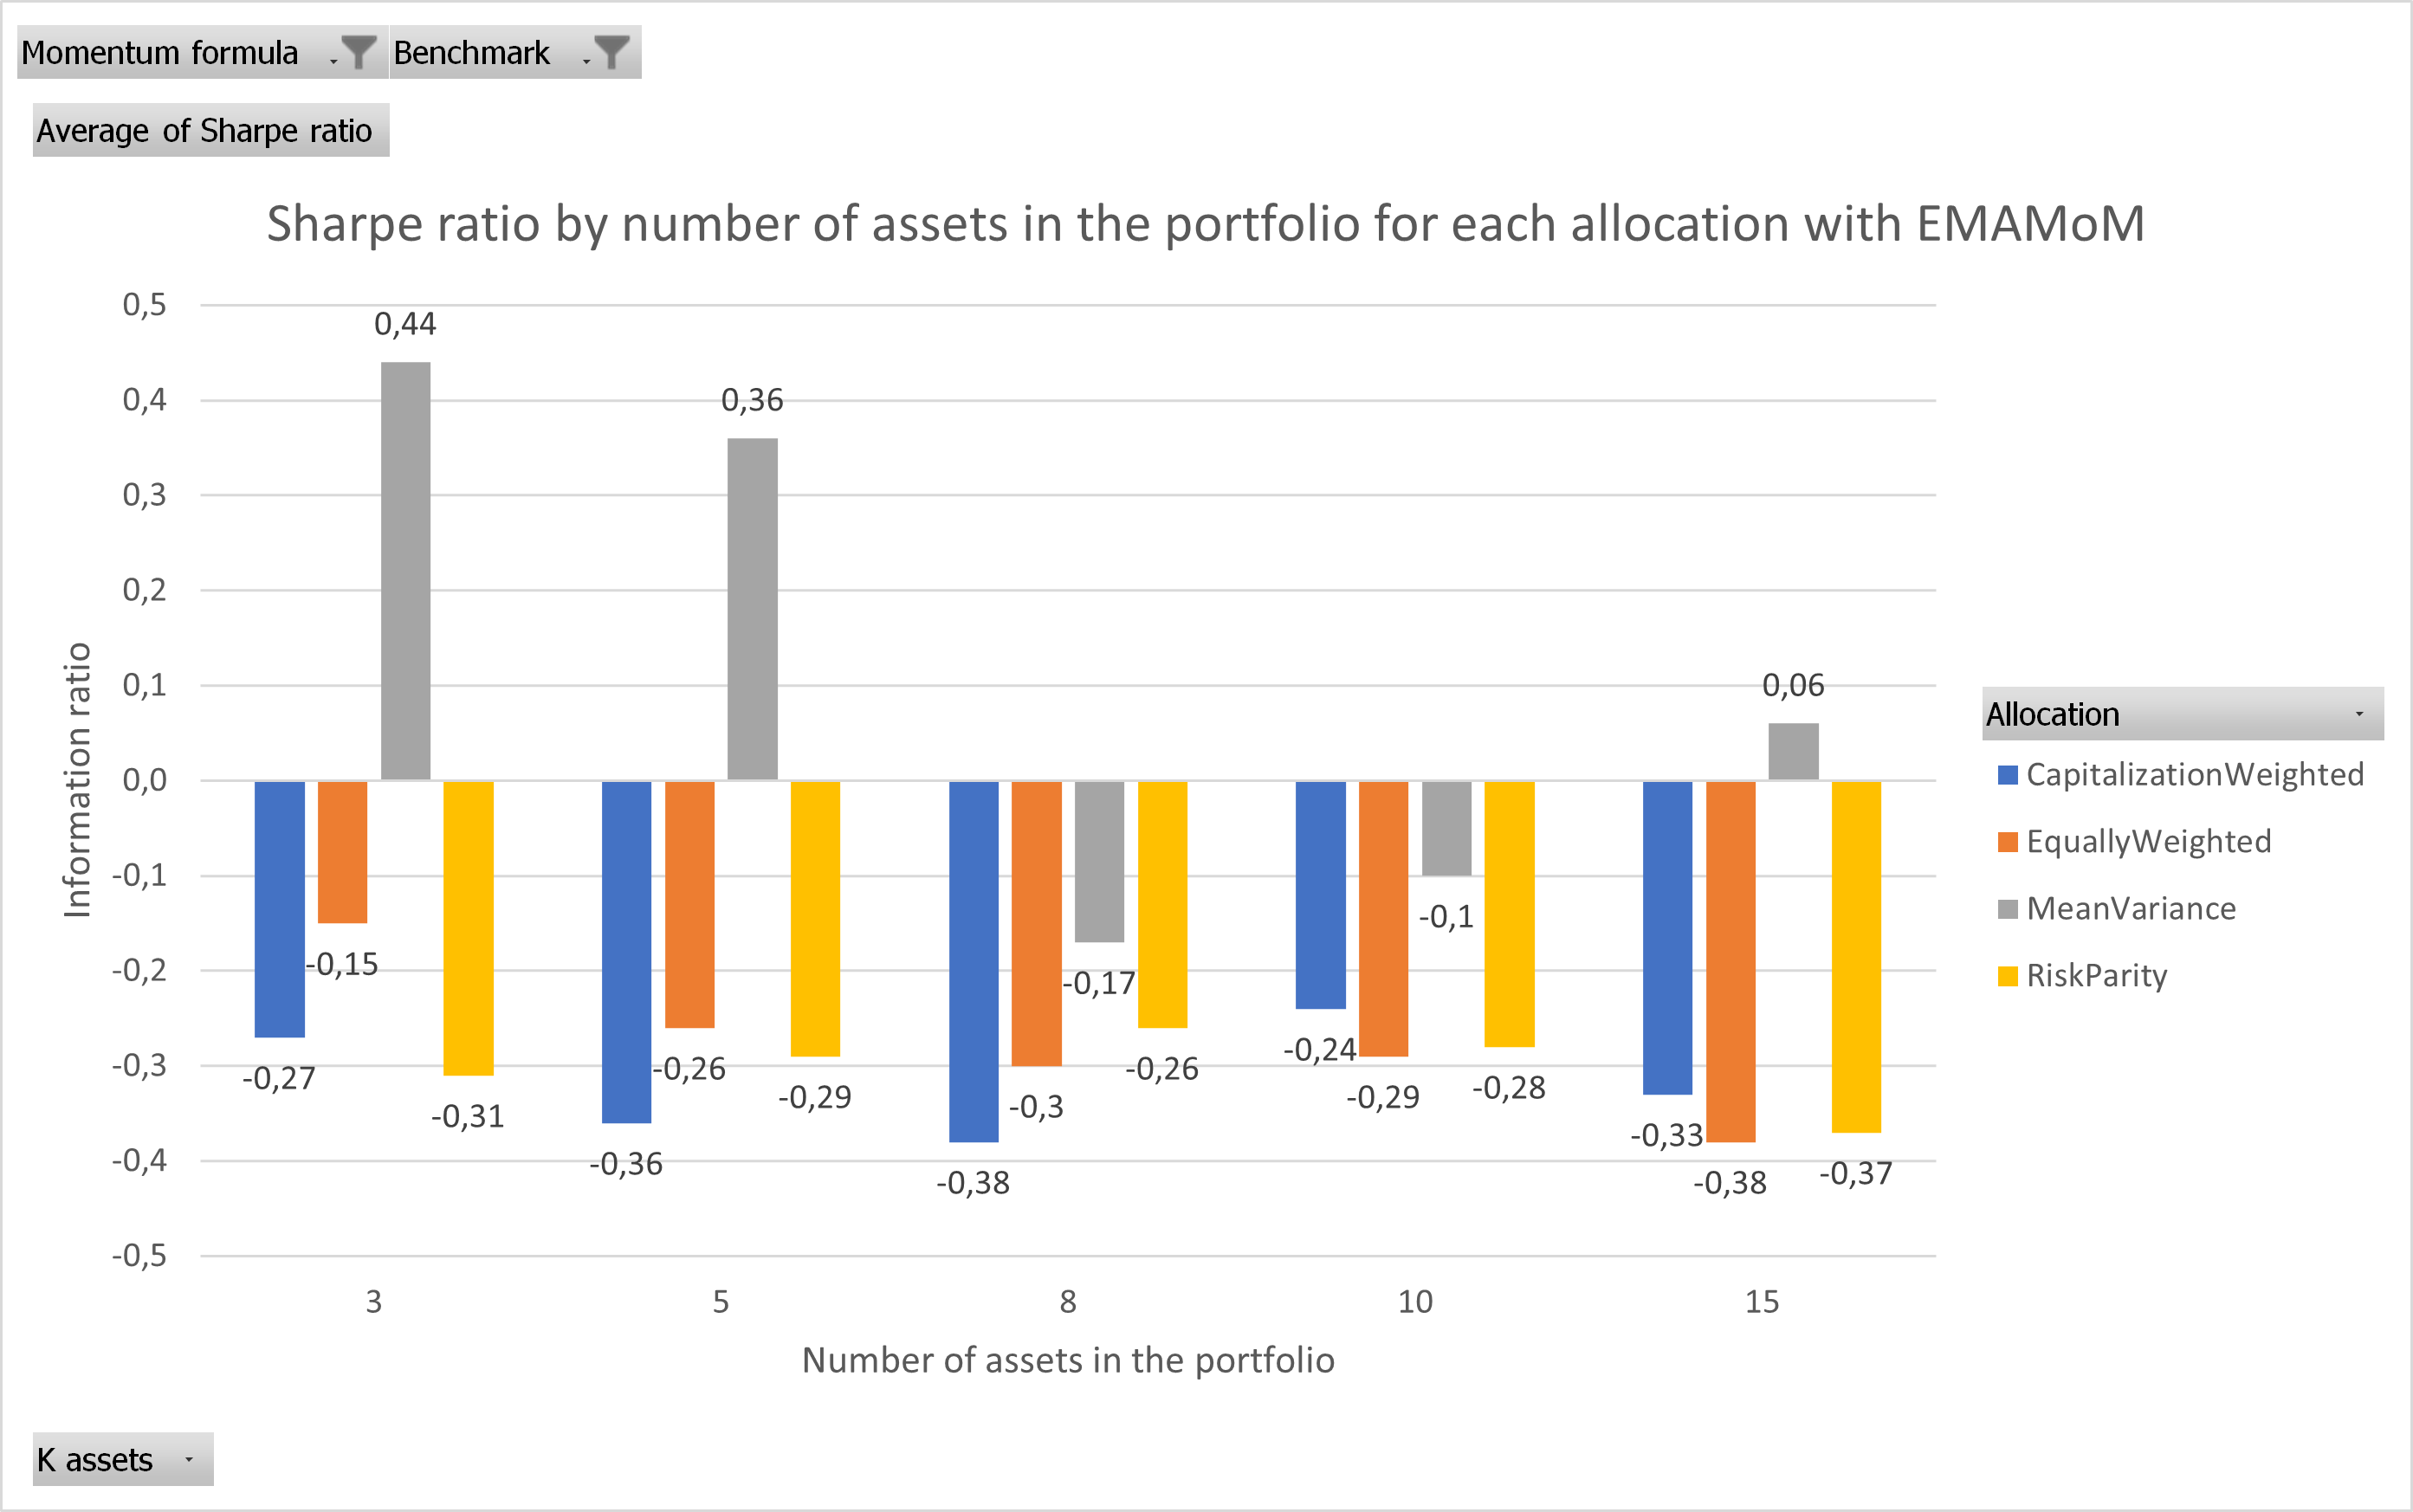
\includegraphics[width=0.75\linewidth]{absolute_management/Sharpe ratio_EMAMoM.png}
    \caption{Average Sharpe ratio for each asset allocation method with respect to the number of assets selected in the portfolio for the EMA Momentum formula}
    \label{fig:Sharpe ratio EMAMOM}
\end{figure}

\begin{figure}[H] % picture
    \centering
    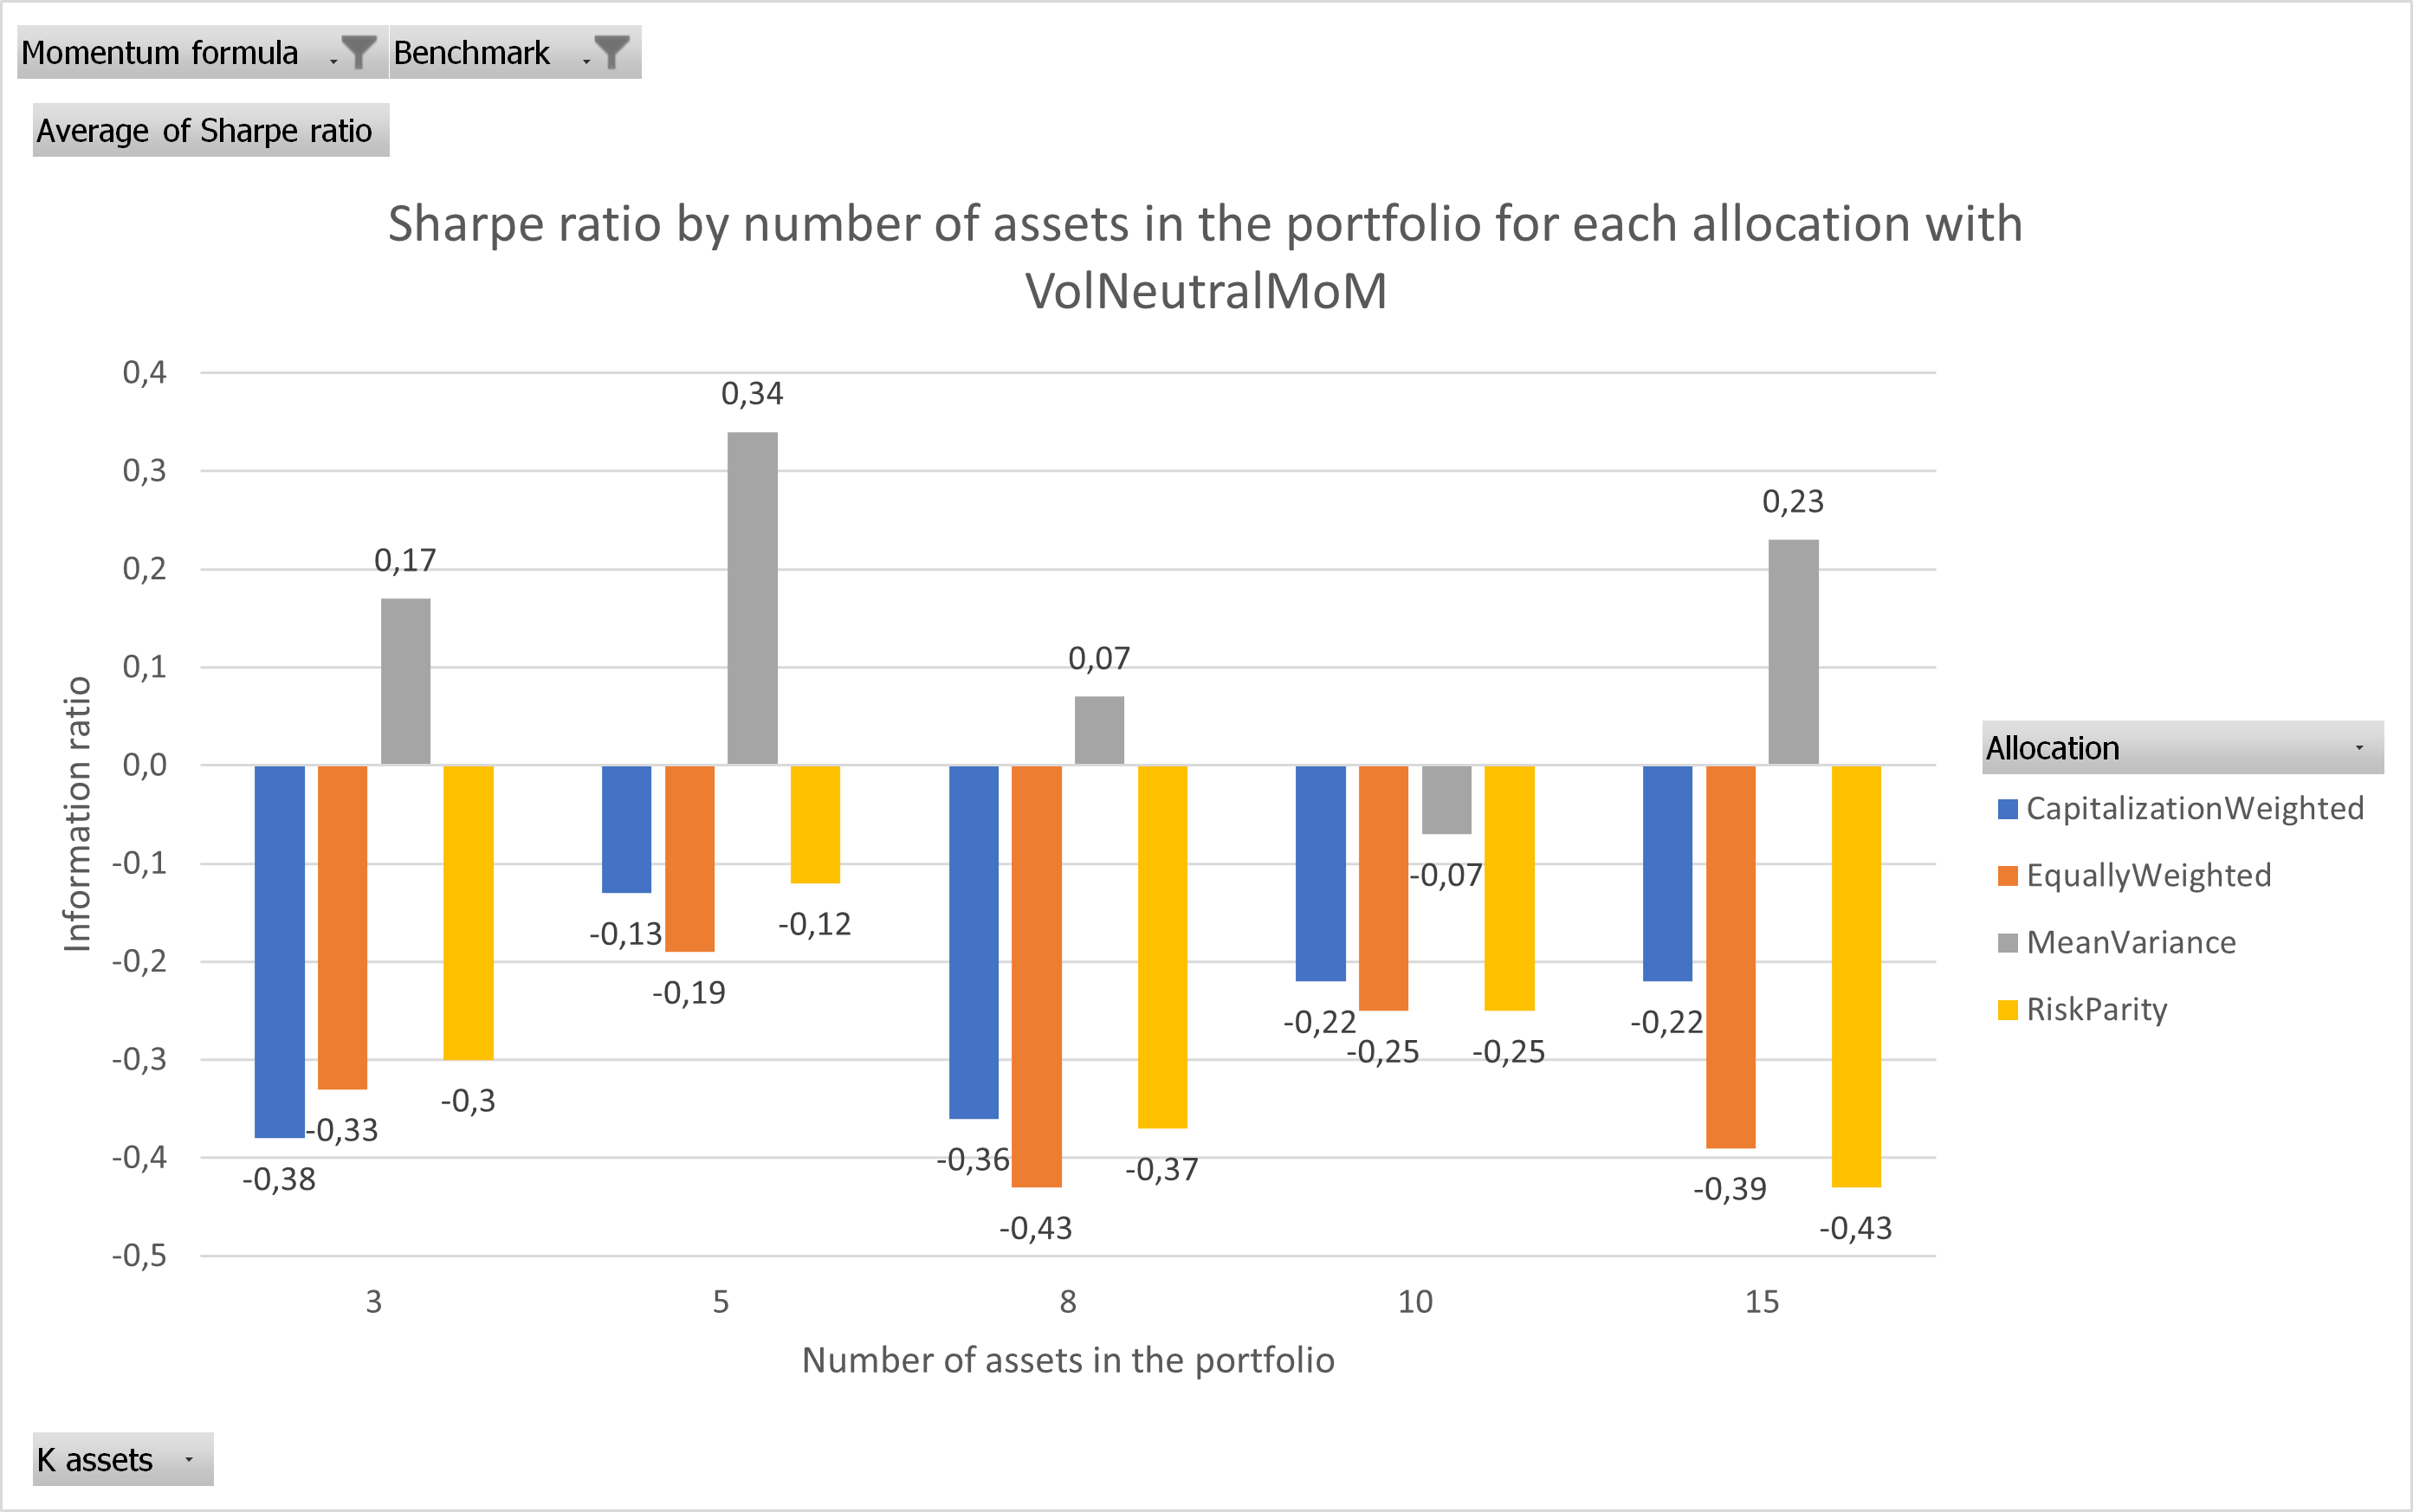
\includegraphics[width=0.75\linewidth]{absolute_management/Sharpe ratio VolNeutalMoM.png}
    \caption{Average Sharpe ratio for each asset allocation method with respect to the number of assets selected in the portfolio for the Volatility Neutral Momentum formula}
    \label{fig:Sharpe ratio VolNeutMOM}
\end{figure}

The preceding four charts clearly illustrate that the optimal approach for asset weight allocation is the mean-variance approach, a conclusion independent of the specific momentum formula employed. This outcome is unsurprising as the mean-variance approach allocates more weight to securities exhibiting a balanced risk/return profile. Notably, the performance of equally weighted and risk parity approaches is suboptimal, aligning with expectations. Allocating equal weights, whether based on risk or not, imposes constraints on potential returns by not favoring the most promising assets. It is pertinent to acknowledge that momentum strategies, due to their nature of selecting the best-performing assets, are inherently associated with elevated risk levels. This phenomenon is exacerbated in the case of the capitalization-weighted approach, where the best-performing assets are more likely to be small-capitalization assets. Consequently, the allocation method appears to contradict our initial conviction that the winners will continue to outperform, as posited by Titman et al. (1993) \cite{Titman1993}.\newline
Moreover, it is noteworthy that the optimal portfolio size, as evaluated from the perspective of the Sharpe ratio, consistently converges to 5 assets. This observation remains consistent regardless of the specific momentum formula utilized. We attribute this result to the focus of momentum selection on high-performing assets, where an increase in portfolio size raises the likelihood of incorporating underperforming assets. As illustrated in Figure \ref{fig:SharpeForAllMoM}, the optimal number of assets for risk-adjusted return is found to be less than 8.

\begin{figure}[H] % picture
    \centering
    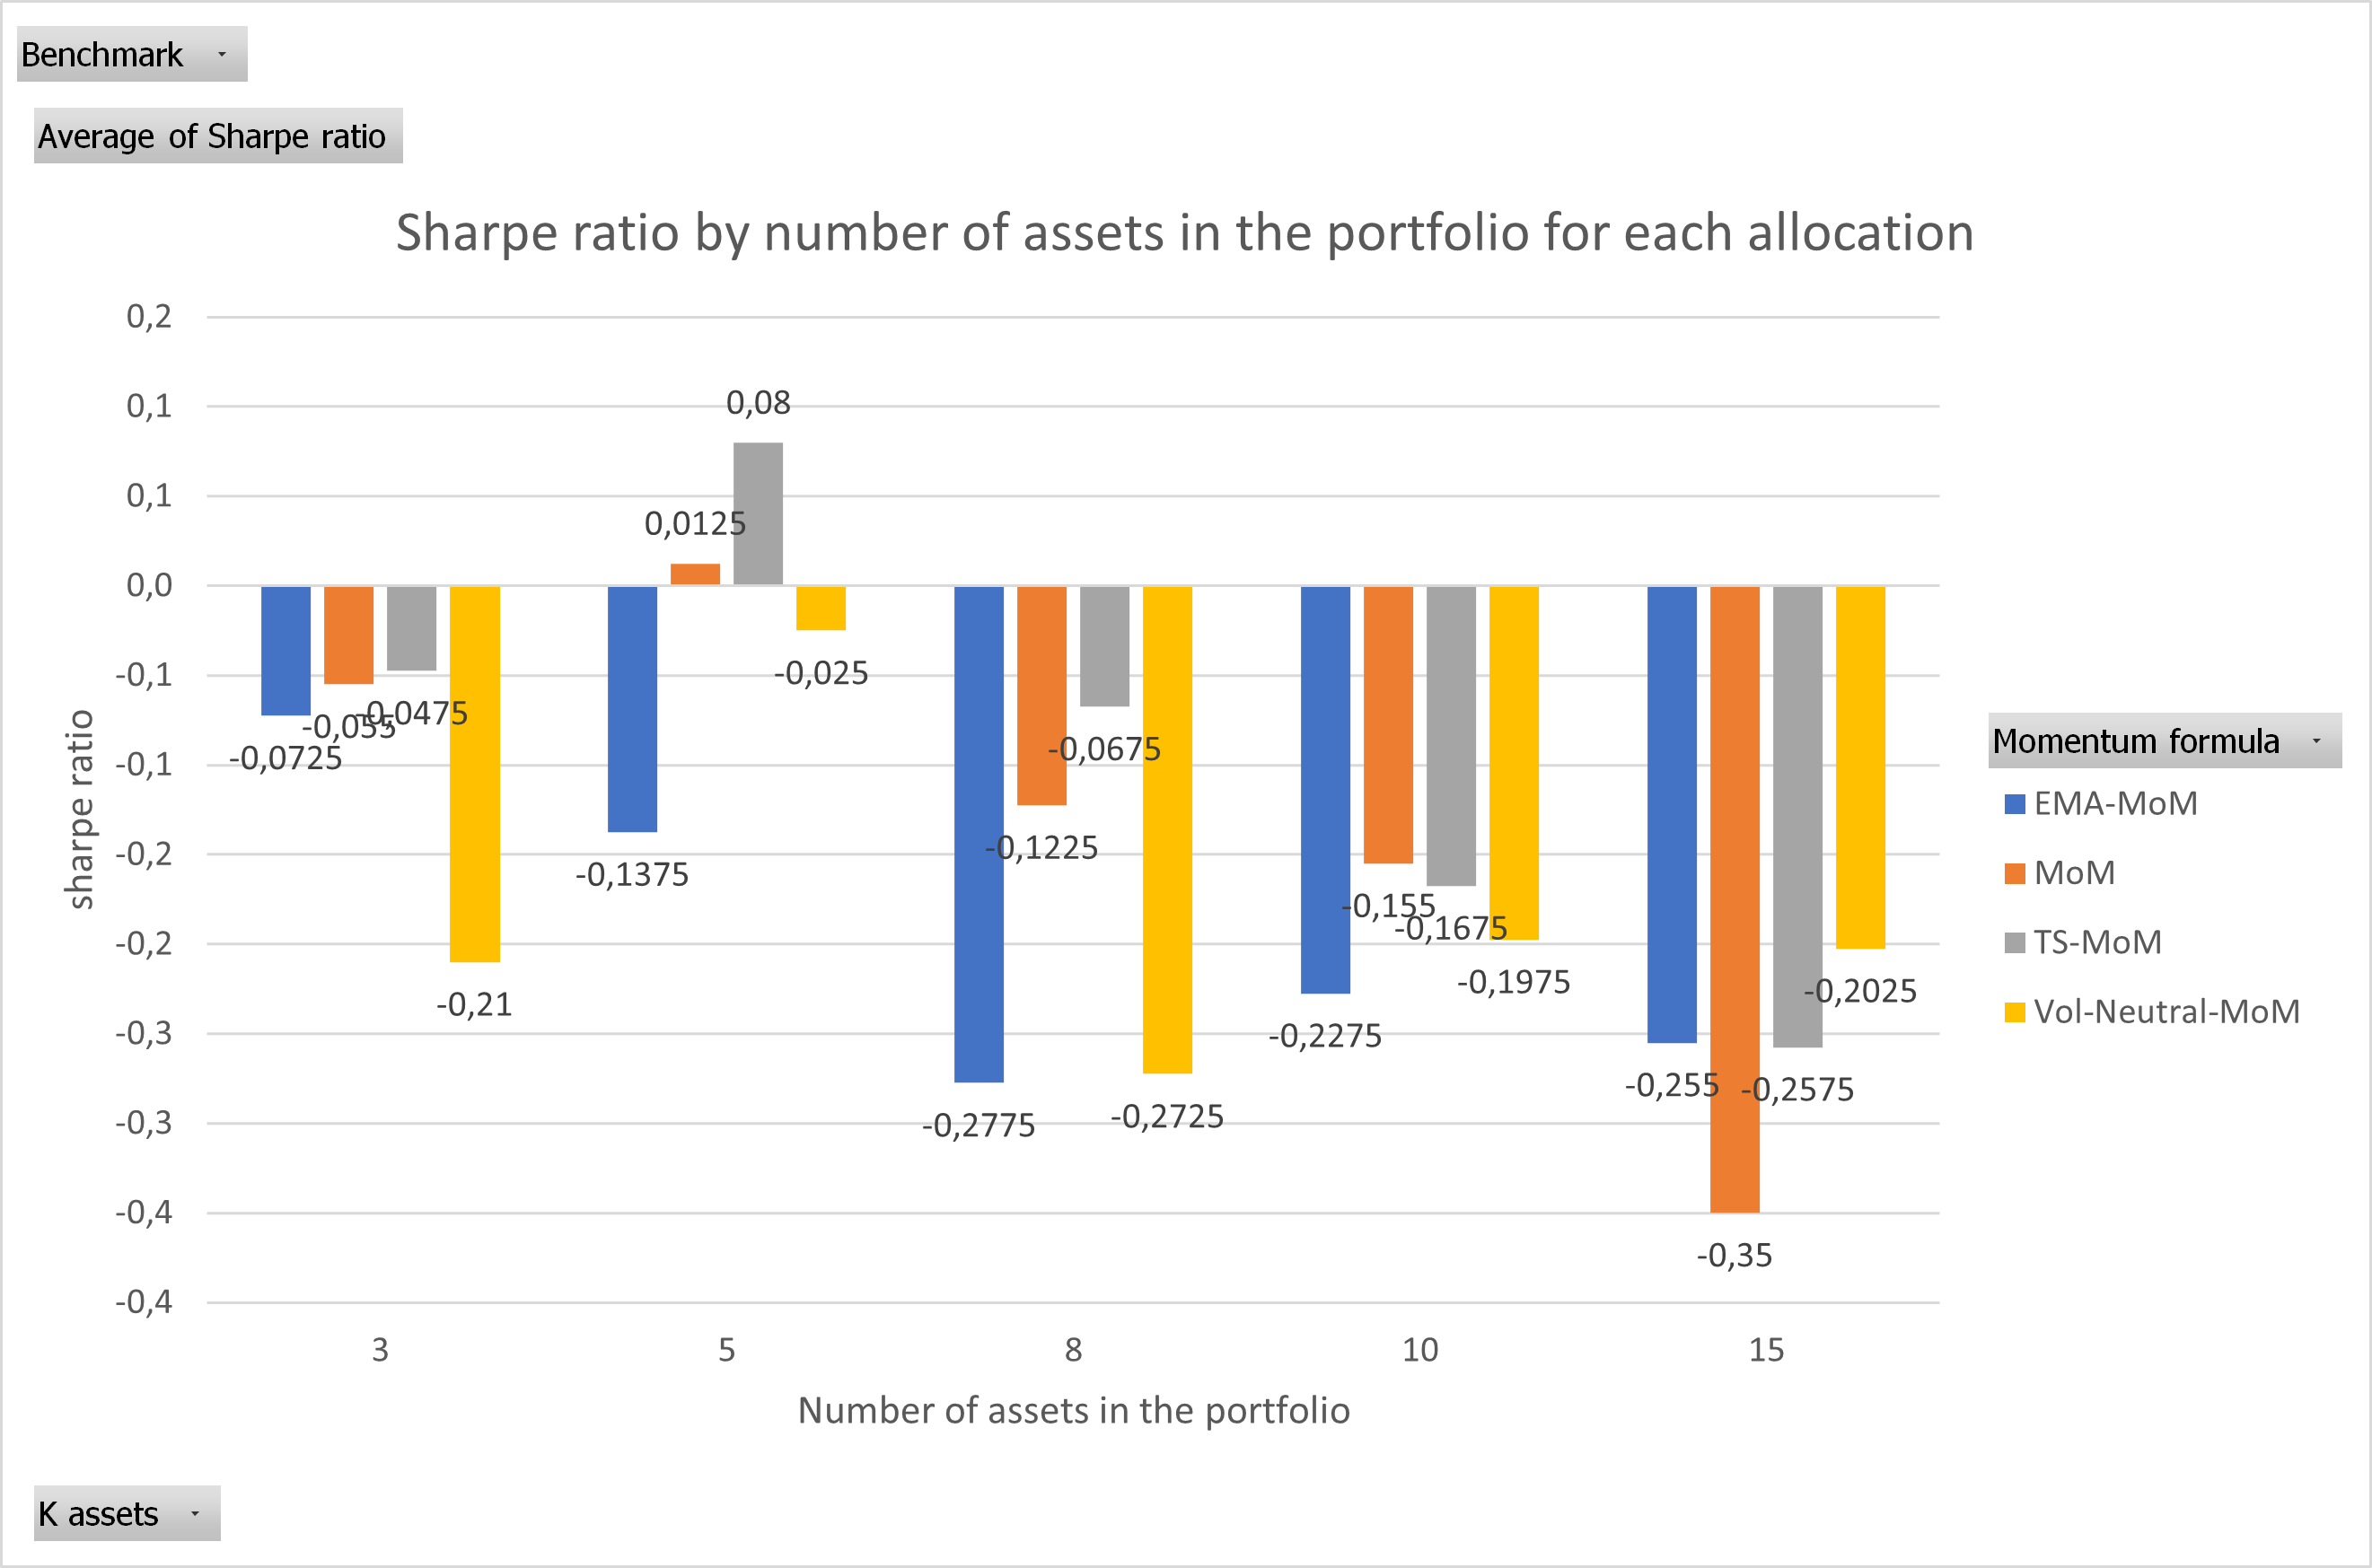
\includegraphics[width=0.75\linewidth]{absolute_management/all_momentum_formula.png}
    \caption{Average Sharpe ratio for each Momentum formula concerning the number of assets selected in the portfolio}
    \label{fig:SharpeForAllMoM}
\end{figure}

Nevertheless, caution must be exercised to avoid an overly low number of assets, as observed in the diversification of idiosyncratic risk and winner volatility, as depicted in Figure \ref{fig:VolForAllMoM}. A balanced portfolio appears to have an optimal number of around 5 assets, considering the need for diversification while acknowledging the heightened volatility of top-performing assets.


\begin{figure}[H] % picture
    \centering
    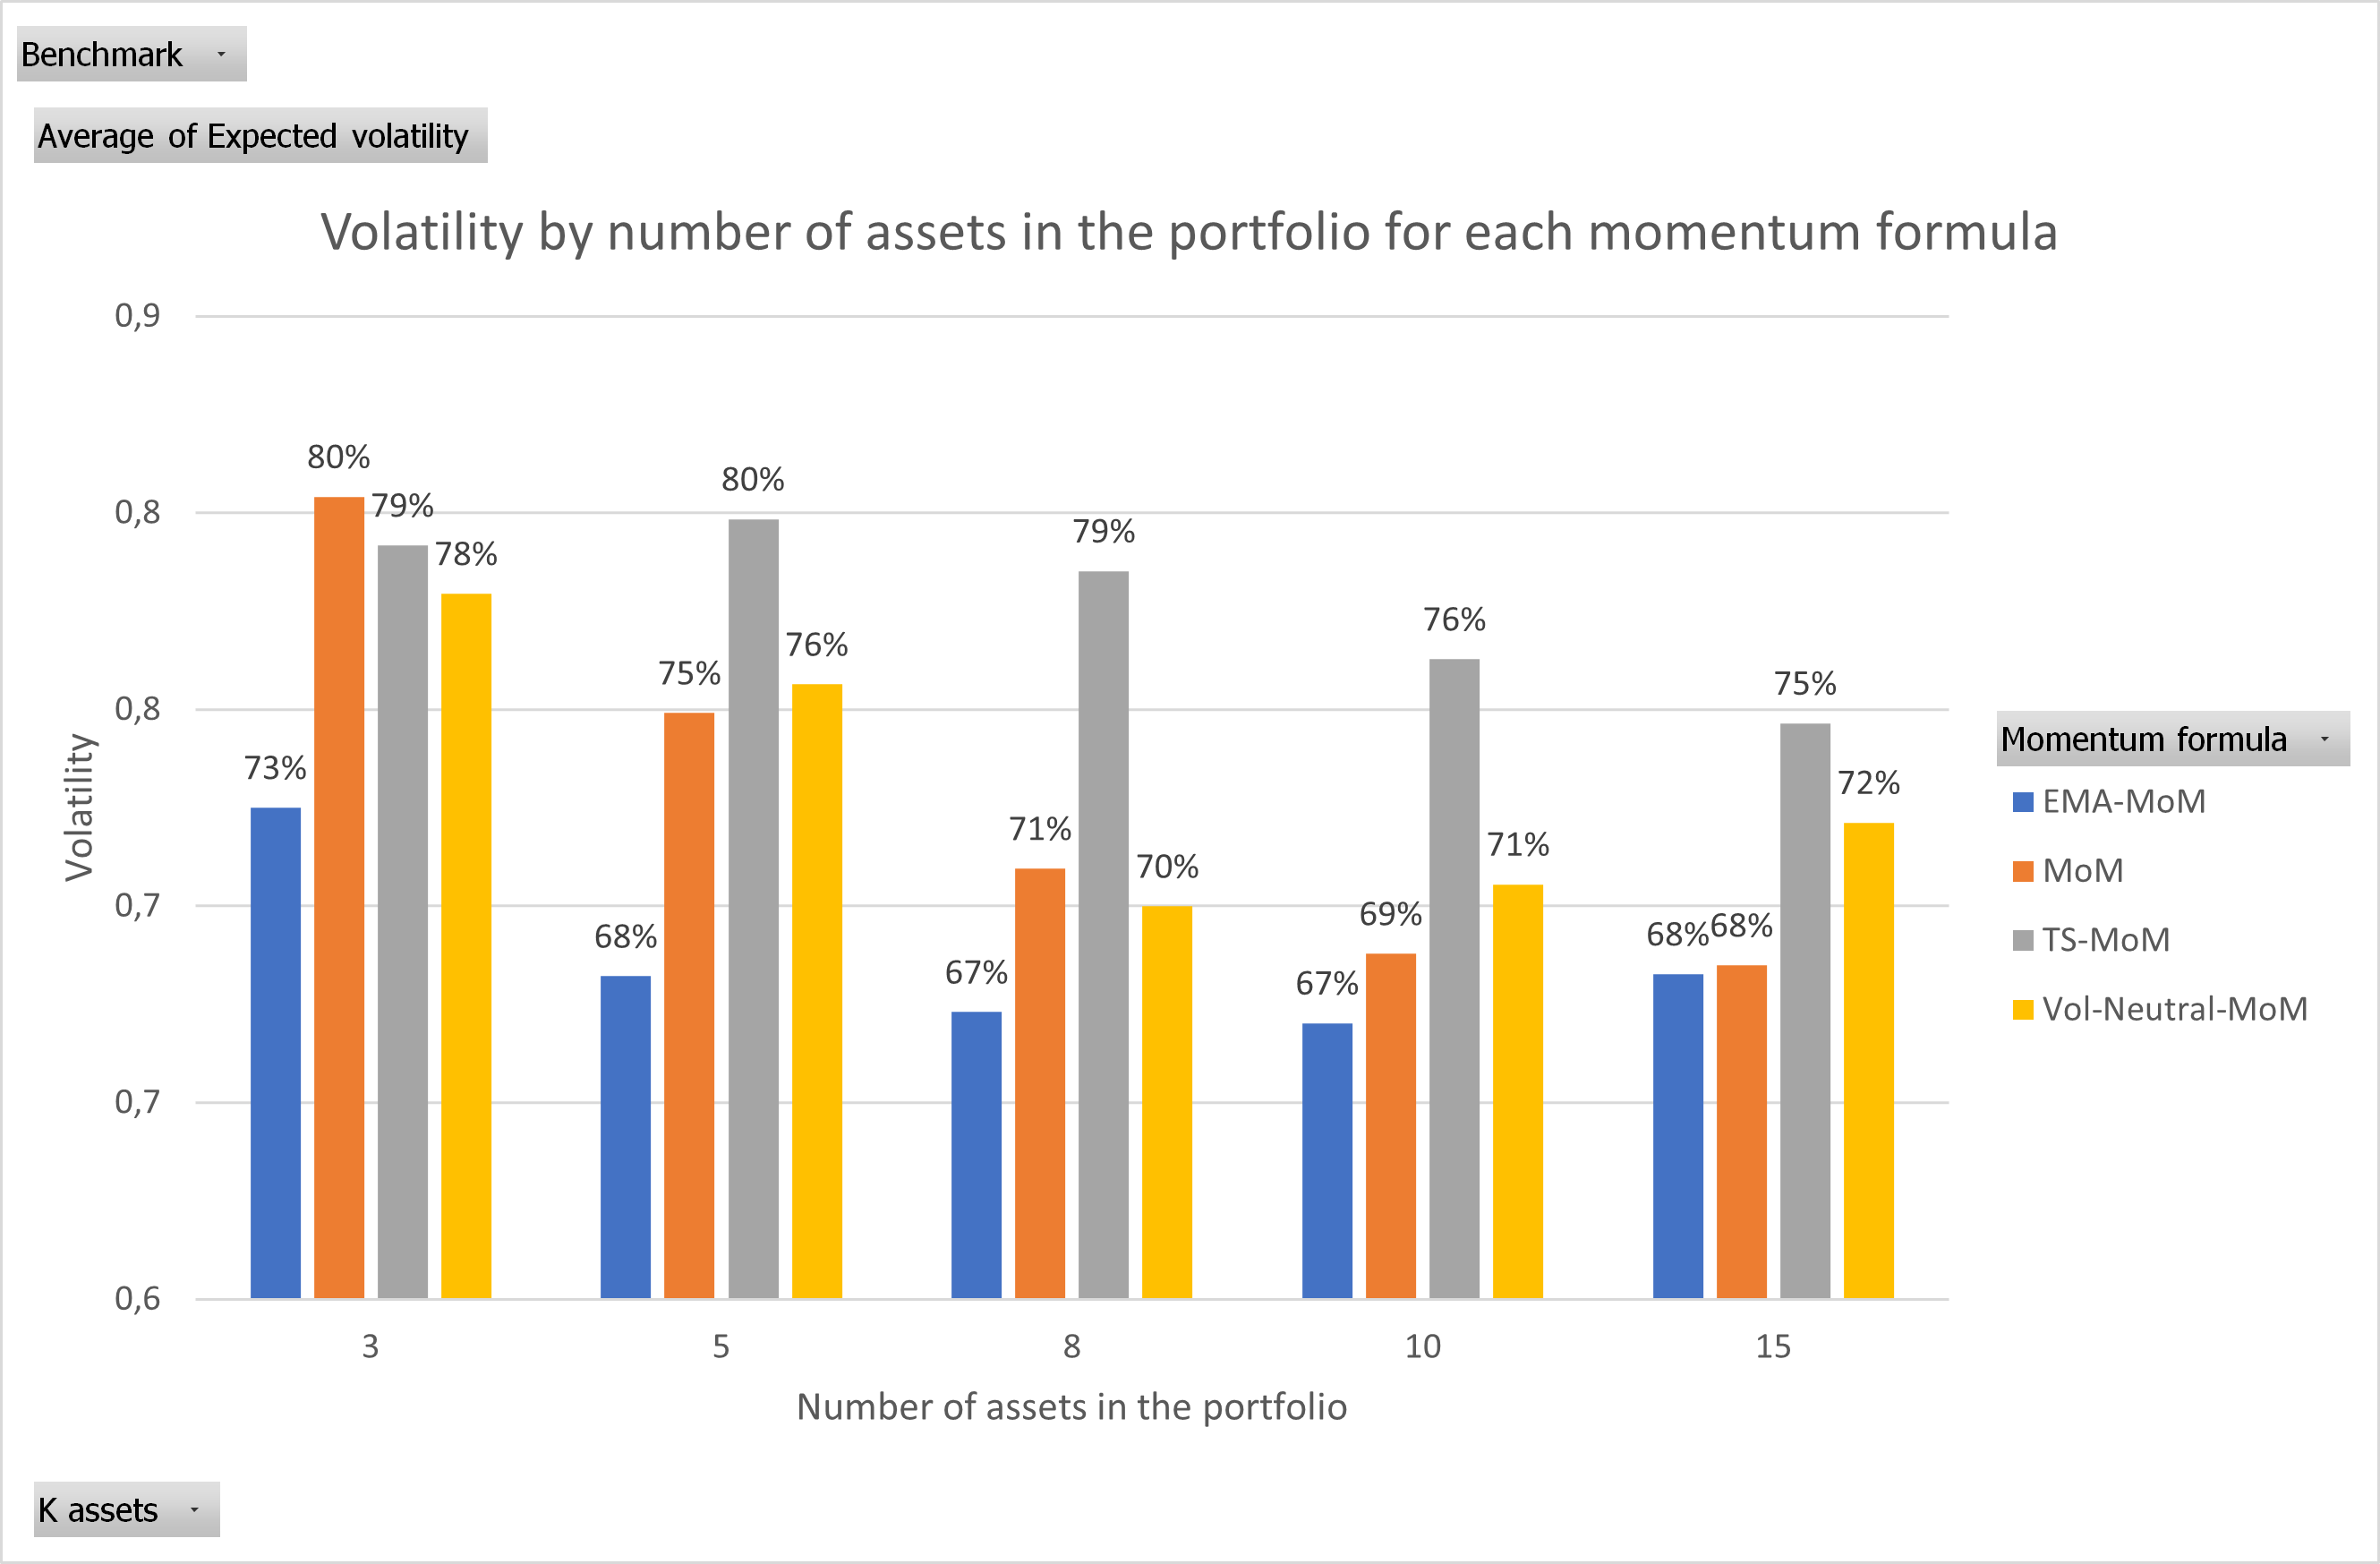
\includegraphics[width=0.75\linewidth]{absolute_management/all_momentum_formula_vol.png}
    \caption{Average Volatility for each Momentum formula with respect to the number of assets selected in the portfolio}
    \label{fig:VolForAllMoM}
\end{figure}

In conclusion, from an absolute performance perspective, the time series momentum formula consistently emerges as the best-performing among the considered momentum formulas, irrespective of the asset allocation method. The average Sharpe ratio, regardless of the number of assets in the portfolio, underscores the superior performance of the time series momentum formula, as demonstrated below \ref{fig:sharpe_by_aloc_for_all_mom}: 
\begin{figure}[H] % picture
    \centering
    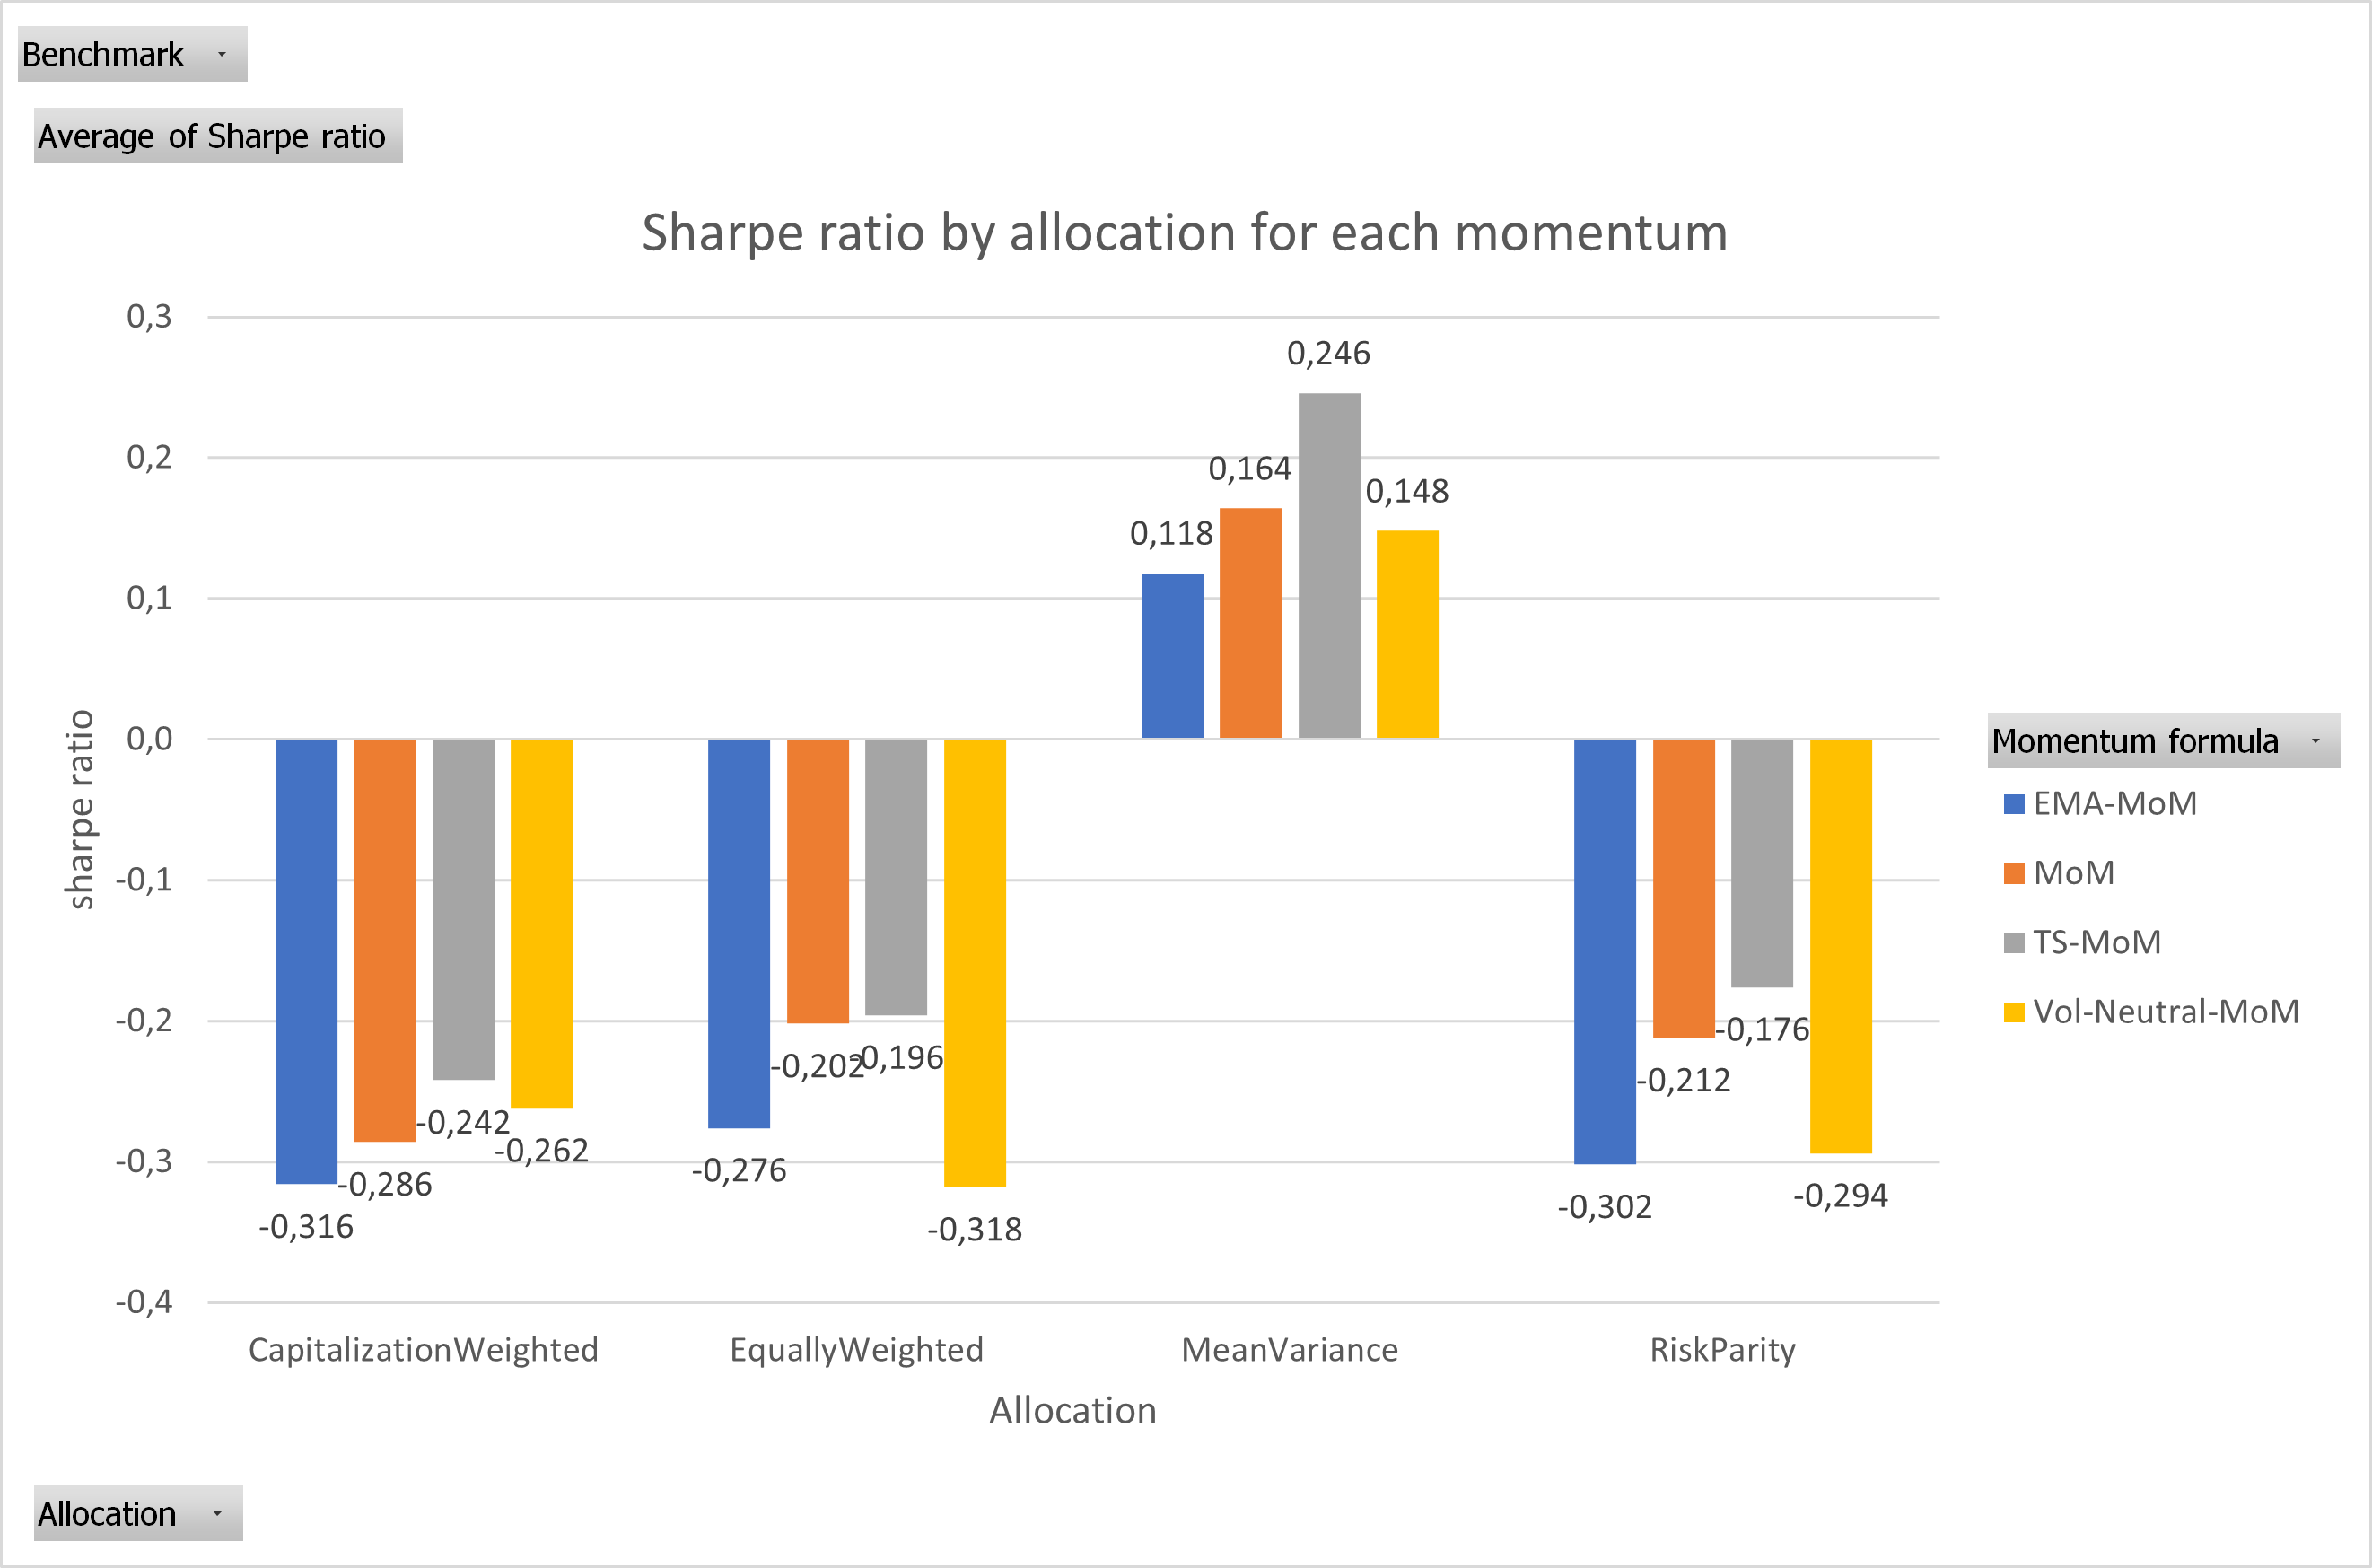
\includegraphics[width=0.75\linewidth]{absolute_management/sharpe_by_aloc_for_all_mom.png}
    \caption{Average Volatility for each Momentum formula with respect to the number of assets selected in the portfolio}
    \label{fig:sharpe_by_aloc_for_all_mom}
\end{figure}

The significance of the results becomes more pronounced when filtering to retain only 5 assets in the portfolio. Notably, the Exponential Moving Average (EMA) momentum formula consistently emerges as the least performing among the formulas considered. This observation suggests that the signal generated by the EMA momentum formula may be excessively volatile, limiting its ability to generate substantial positive returns.

\begin{figure}[H] % picture
    \centering
    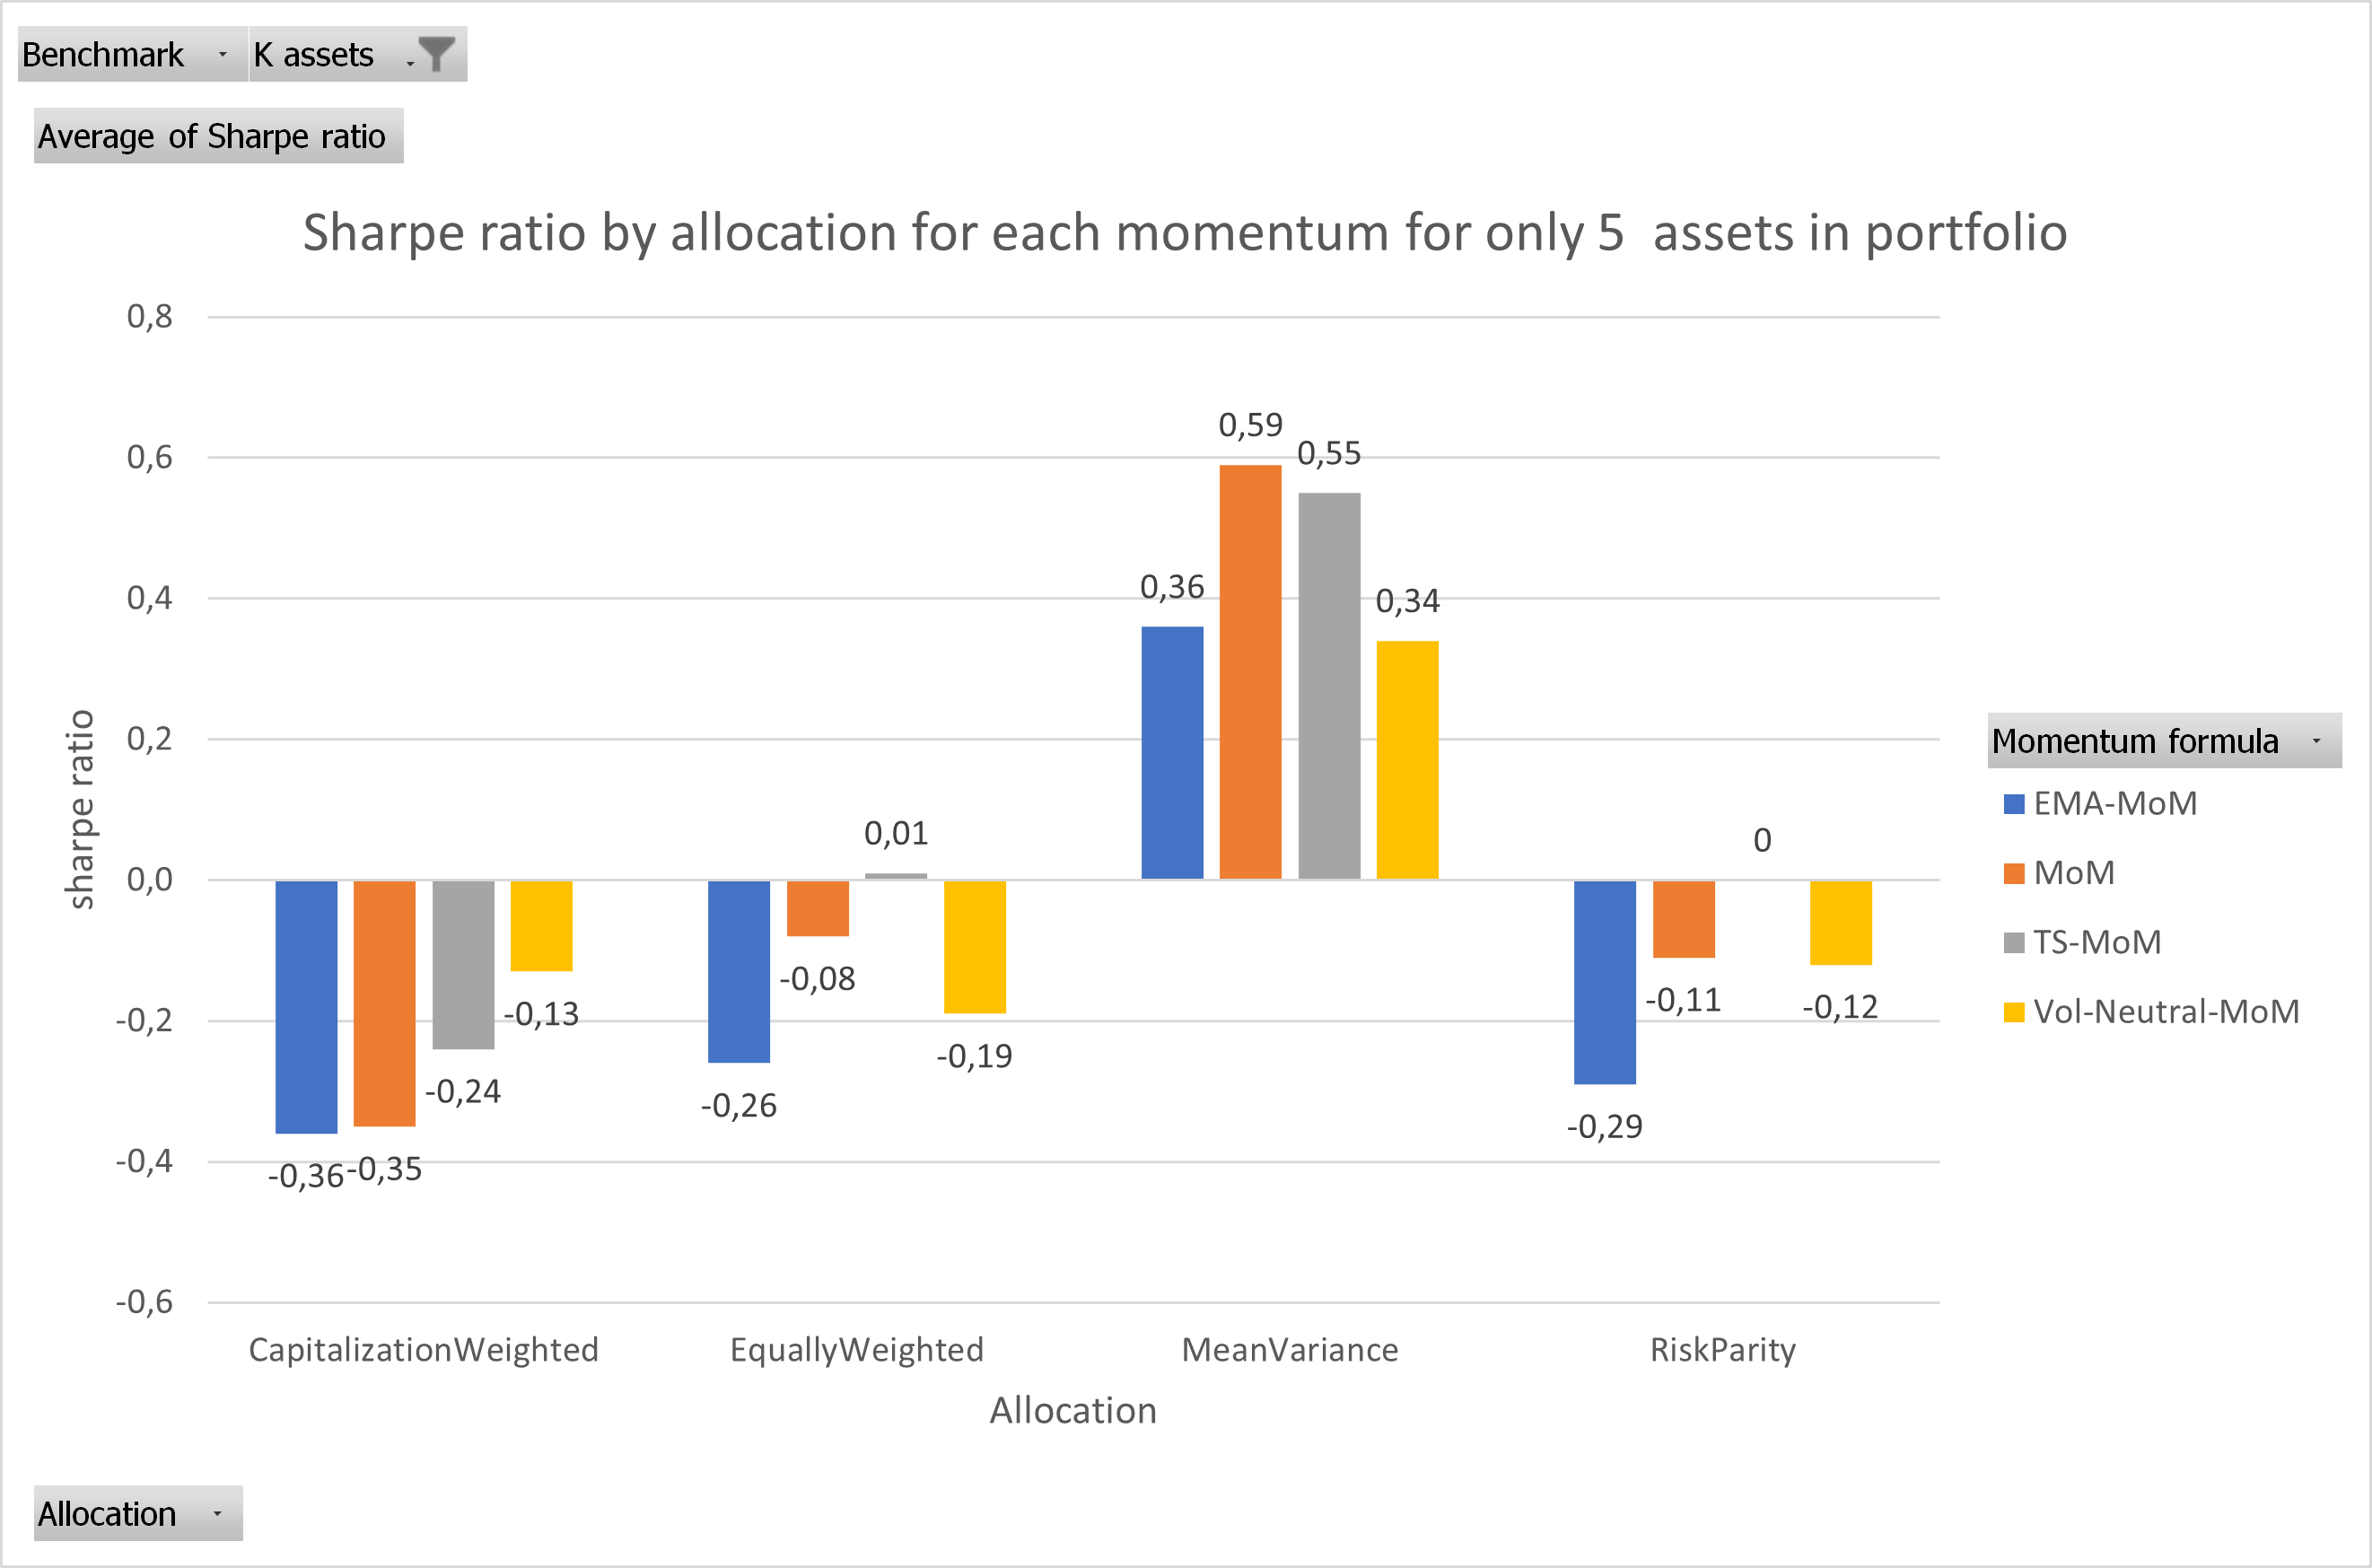
\includegraphics[width=0.75\linewidth]{absolute_management/sharpe_by_aloc_for_all_mom_5_assets.png}
    \caption{Average Volatility for each Momentum formula with respect to the number of assets selected in the portfolio}
    \label{fig:sharpe_by_aloc_for_all_mom5assets}
\end{figure}


\subsubsection{Relative portfolio management style}
In this section we present the result obtained from the backtests in order to conclude on the potential value in using momentum for asset selection. This section will focus on the relative portfolio management framework. The most important metric to consider in this section is the Information ratio as it is an relative risk adjusted measure that quantify the return by relative risk unit. Here the risk is measured with the tracking error. We only consider one benchmarks the BITCOIN. However all the results are presents in the appendix section \ref{sec:appendix}. We display the Information ratio for each momentum formula.

\begin{figure}[H] % picture
    \centering
    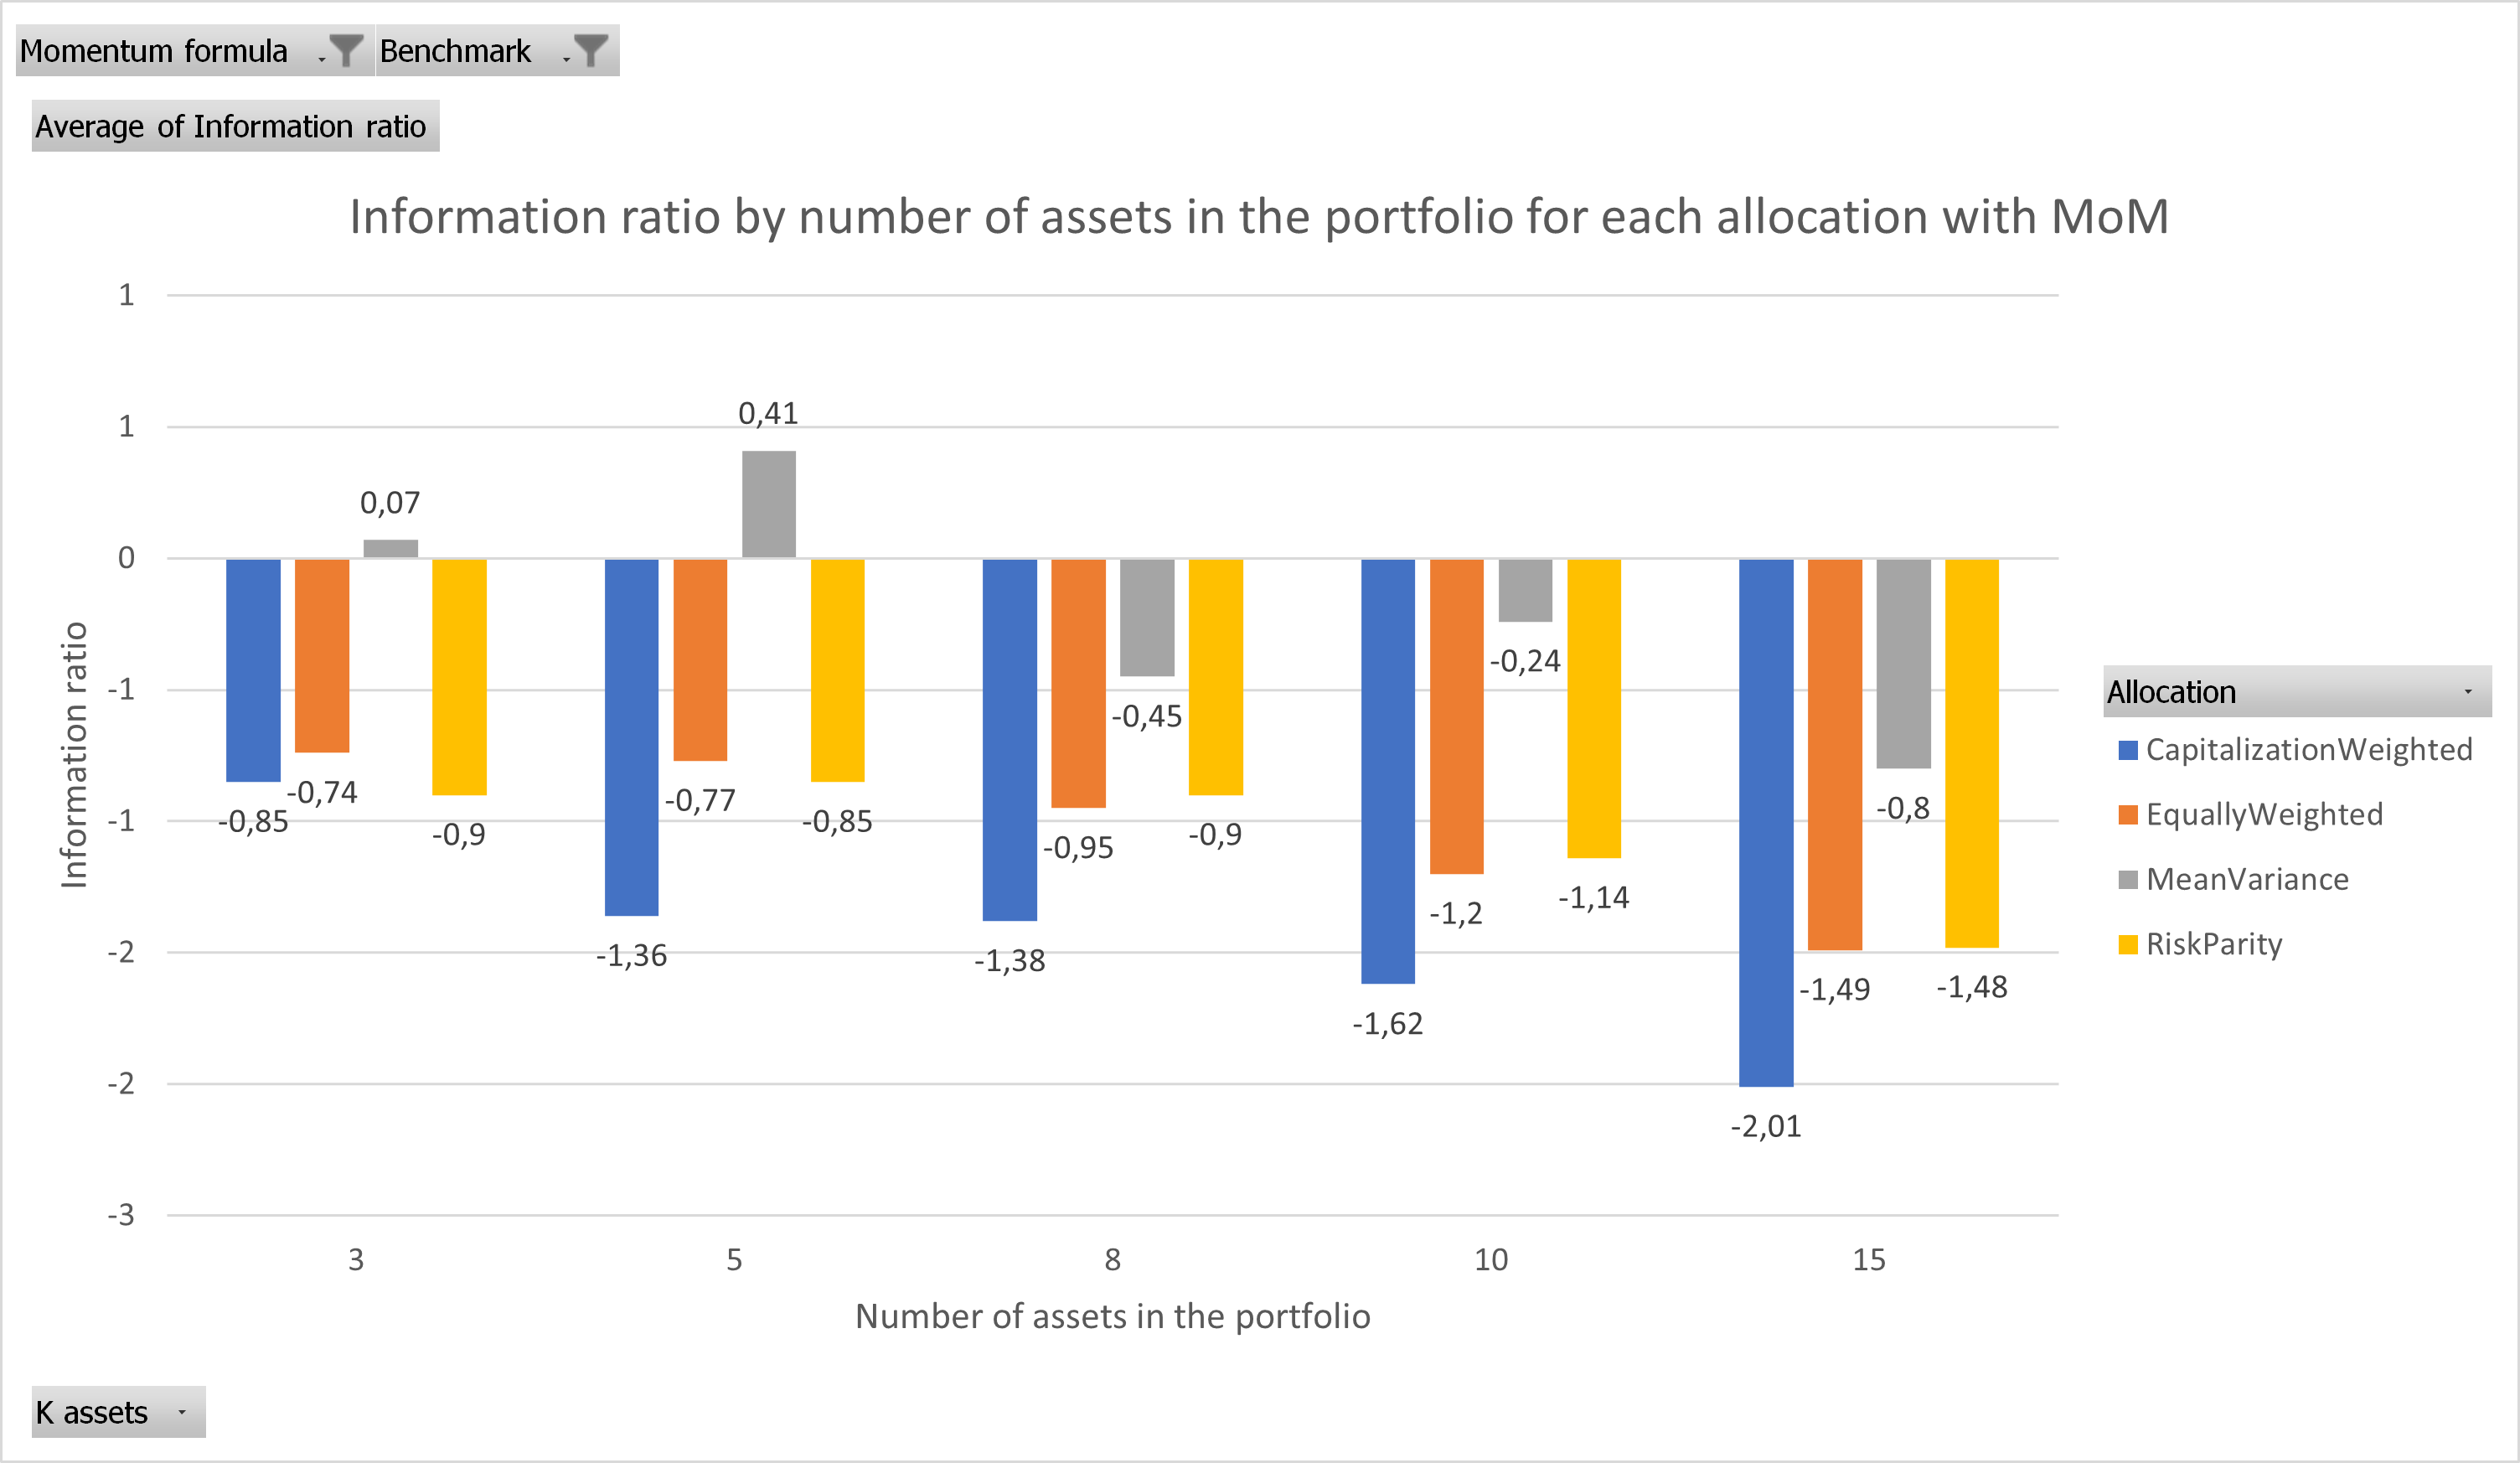
\includegraphics[width=0.75\linewidth]{relative_management/Information ratio MoM_BenchBTC.png}
    \caption{Average Information ratio for each asset allocation method with respect to the number of assets selected in the portfolio for the Price Momentum formula}
    \label{fig:info ratio MoM}
\end{figure}

\begin{figure}[H] % picture
    \centering
    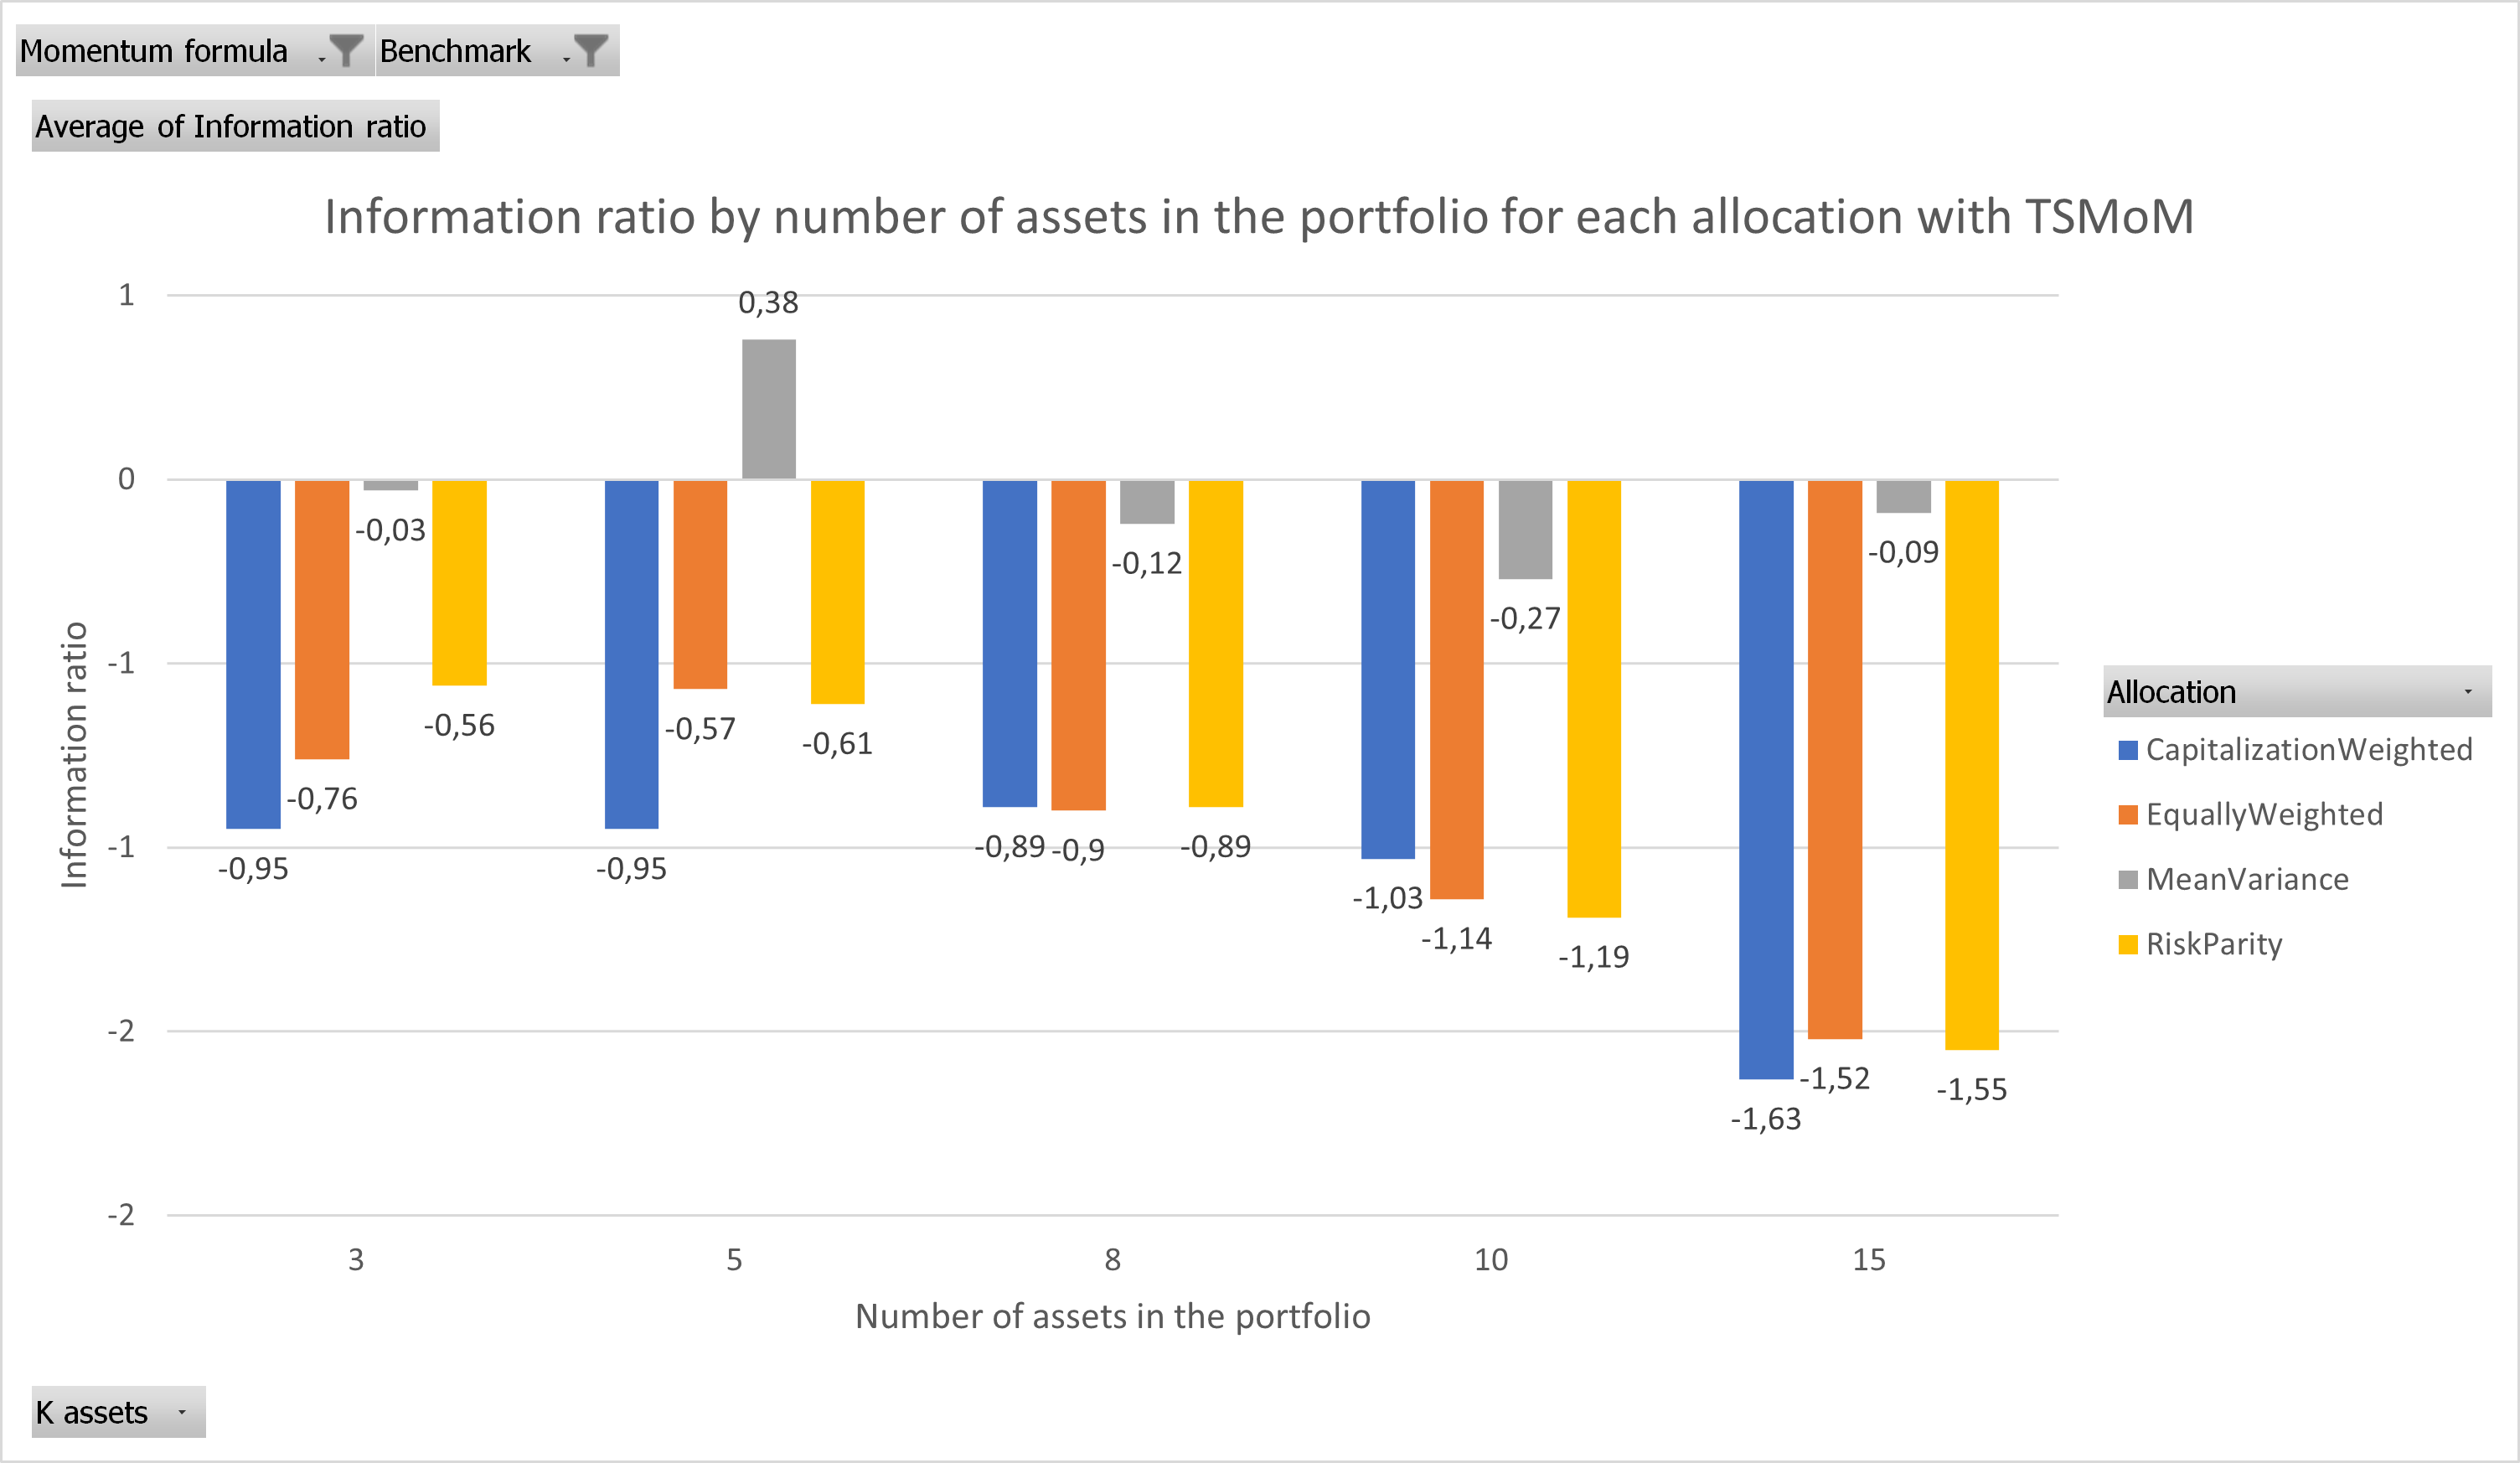
\includegraphics[width=0.75\linewidth]{relative_management/Information ratio TSMoM_BenchBTC.png}
    \caption{Average Information ratio for each asset allocation method with respect to the number of assets selected in the portfolio for the Time Series Momentum formula}
    \label{fig:info ratio TSMOM}
\end{figure}

\begin{figure}[H] % picture
    \centering
    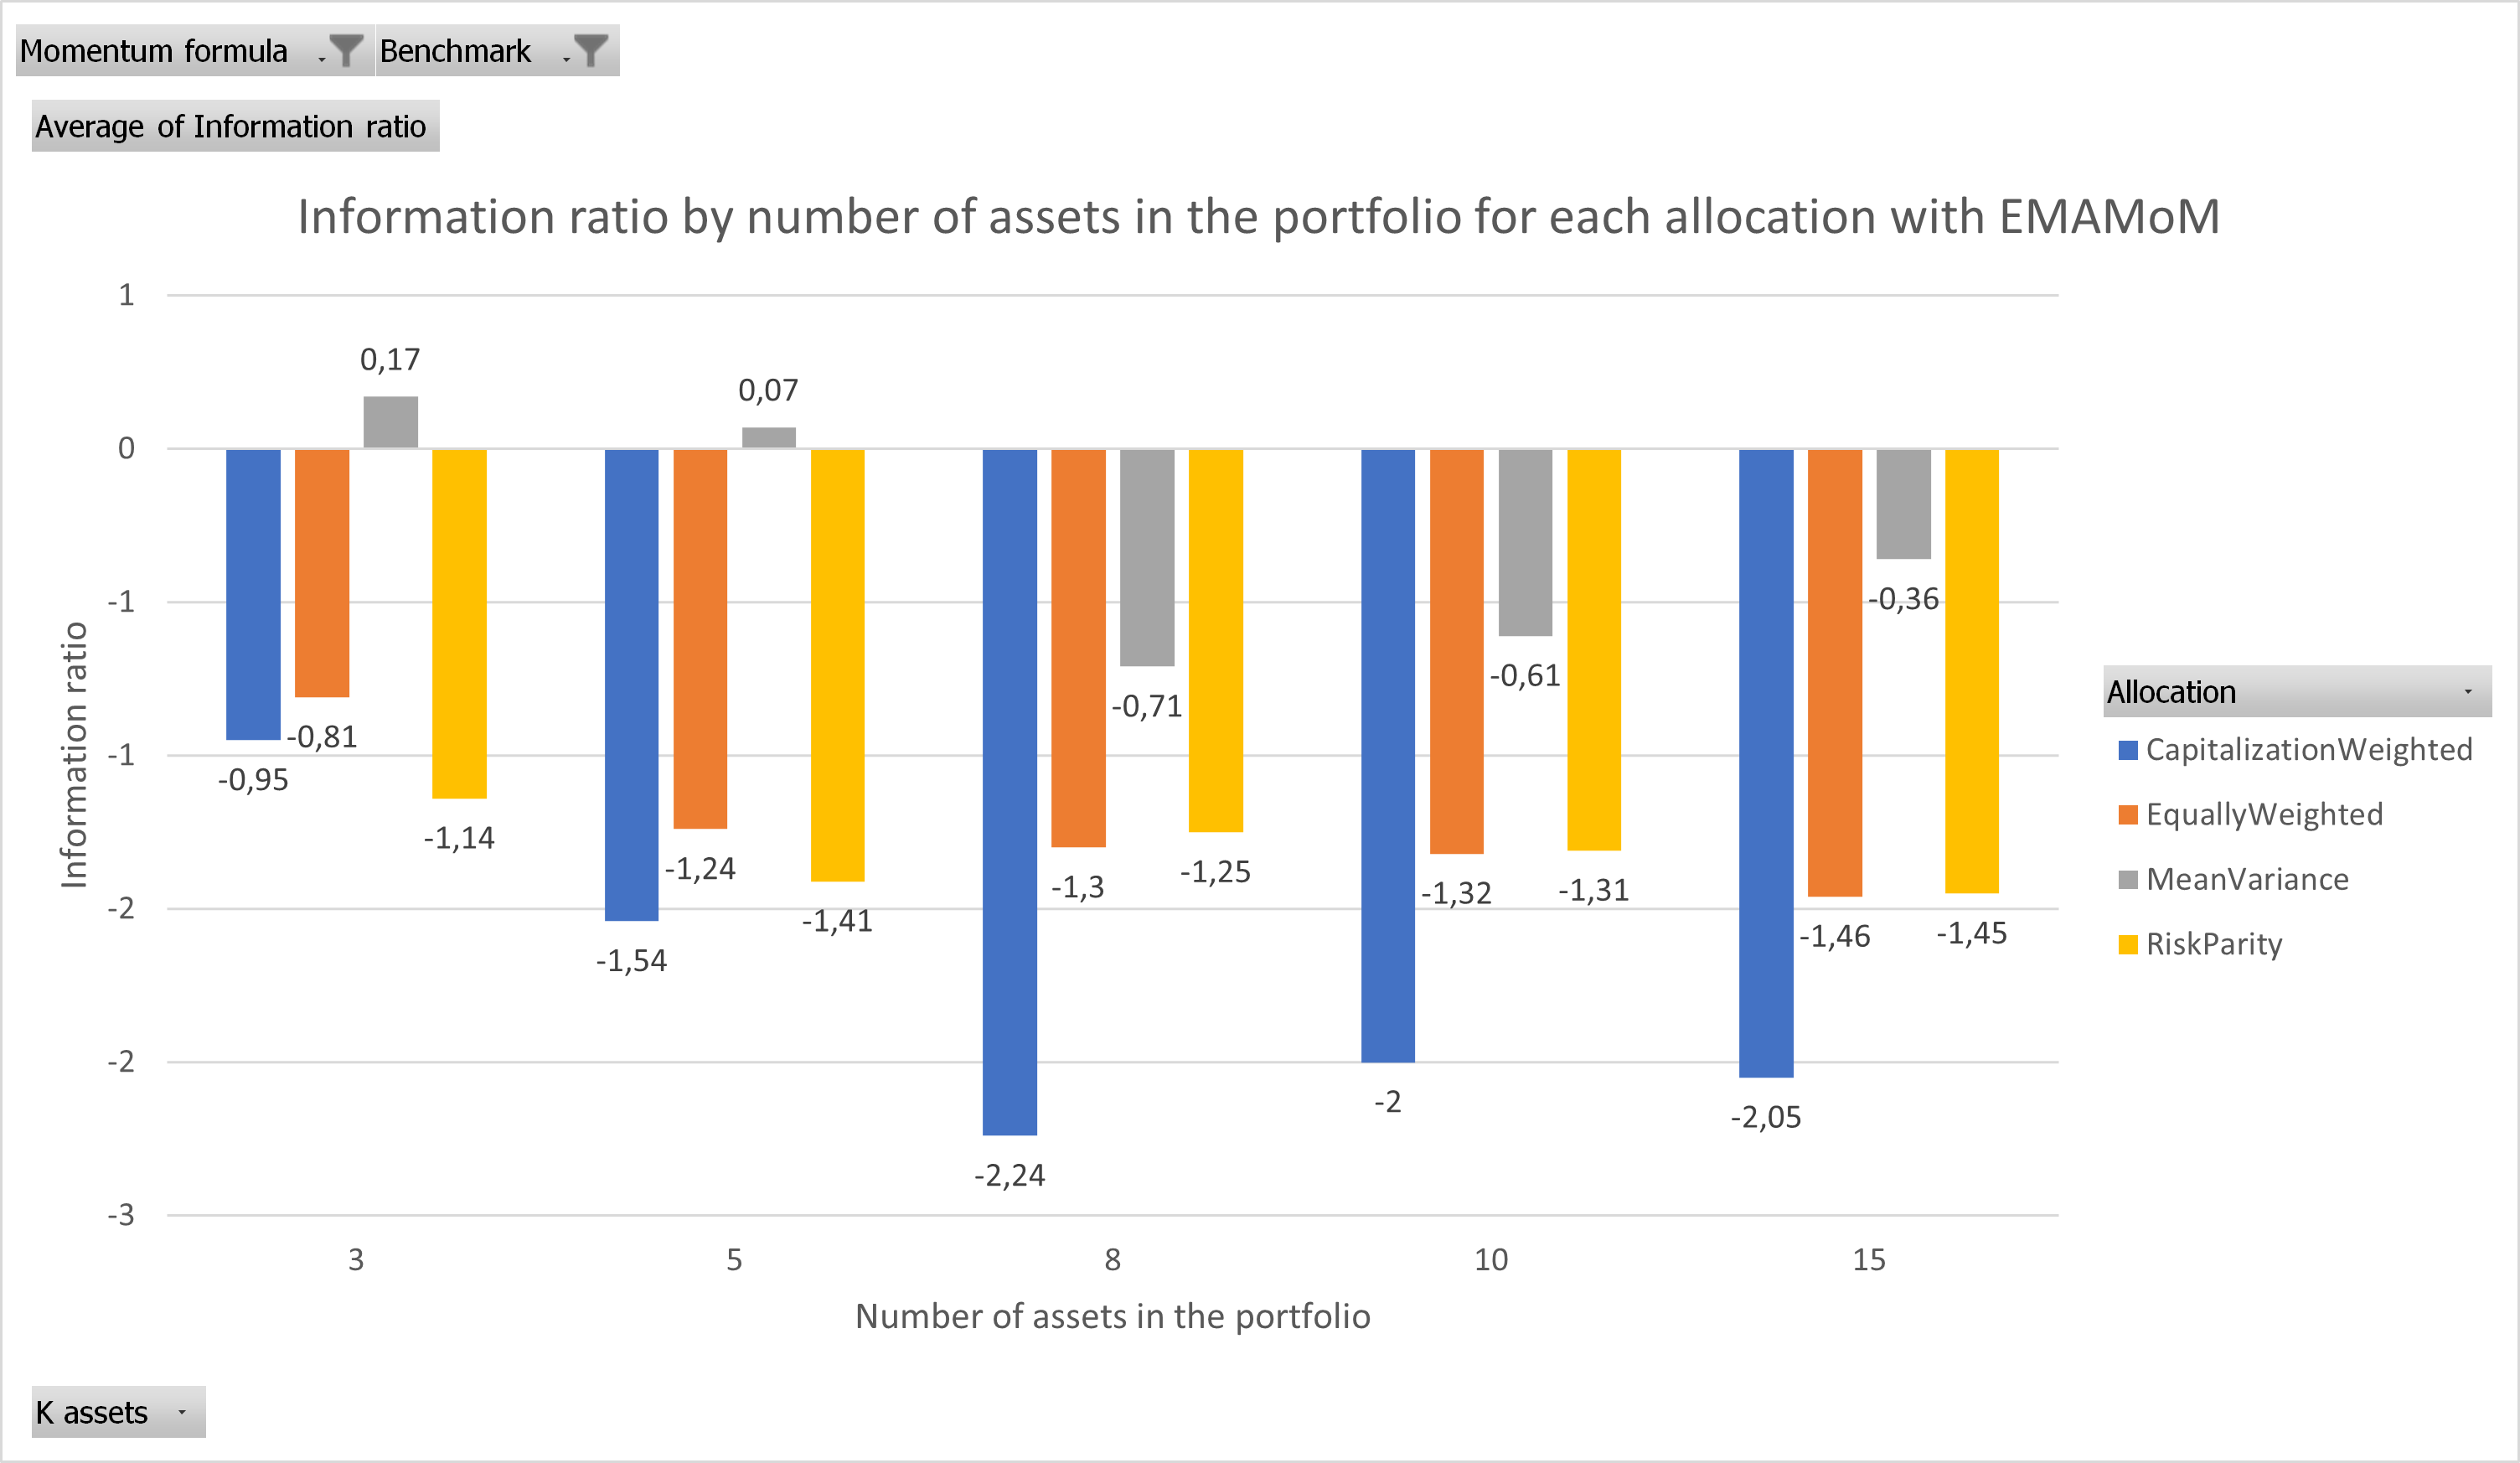
\includegraphics[width=0.75\linewidth]{relative_management/Information ratio_EMAMoM_BenchBTC.png}
    \caption{Average Information ratio for each asset allocation method with respect to the number of assets selected in the portfolio for the EMA Momentum formula}
    \label{fig:info ratio EMAMOM}
\end{figure}

\begin{figure}[H] % picture
    \centering
    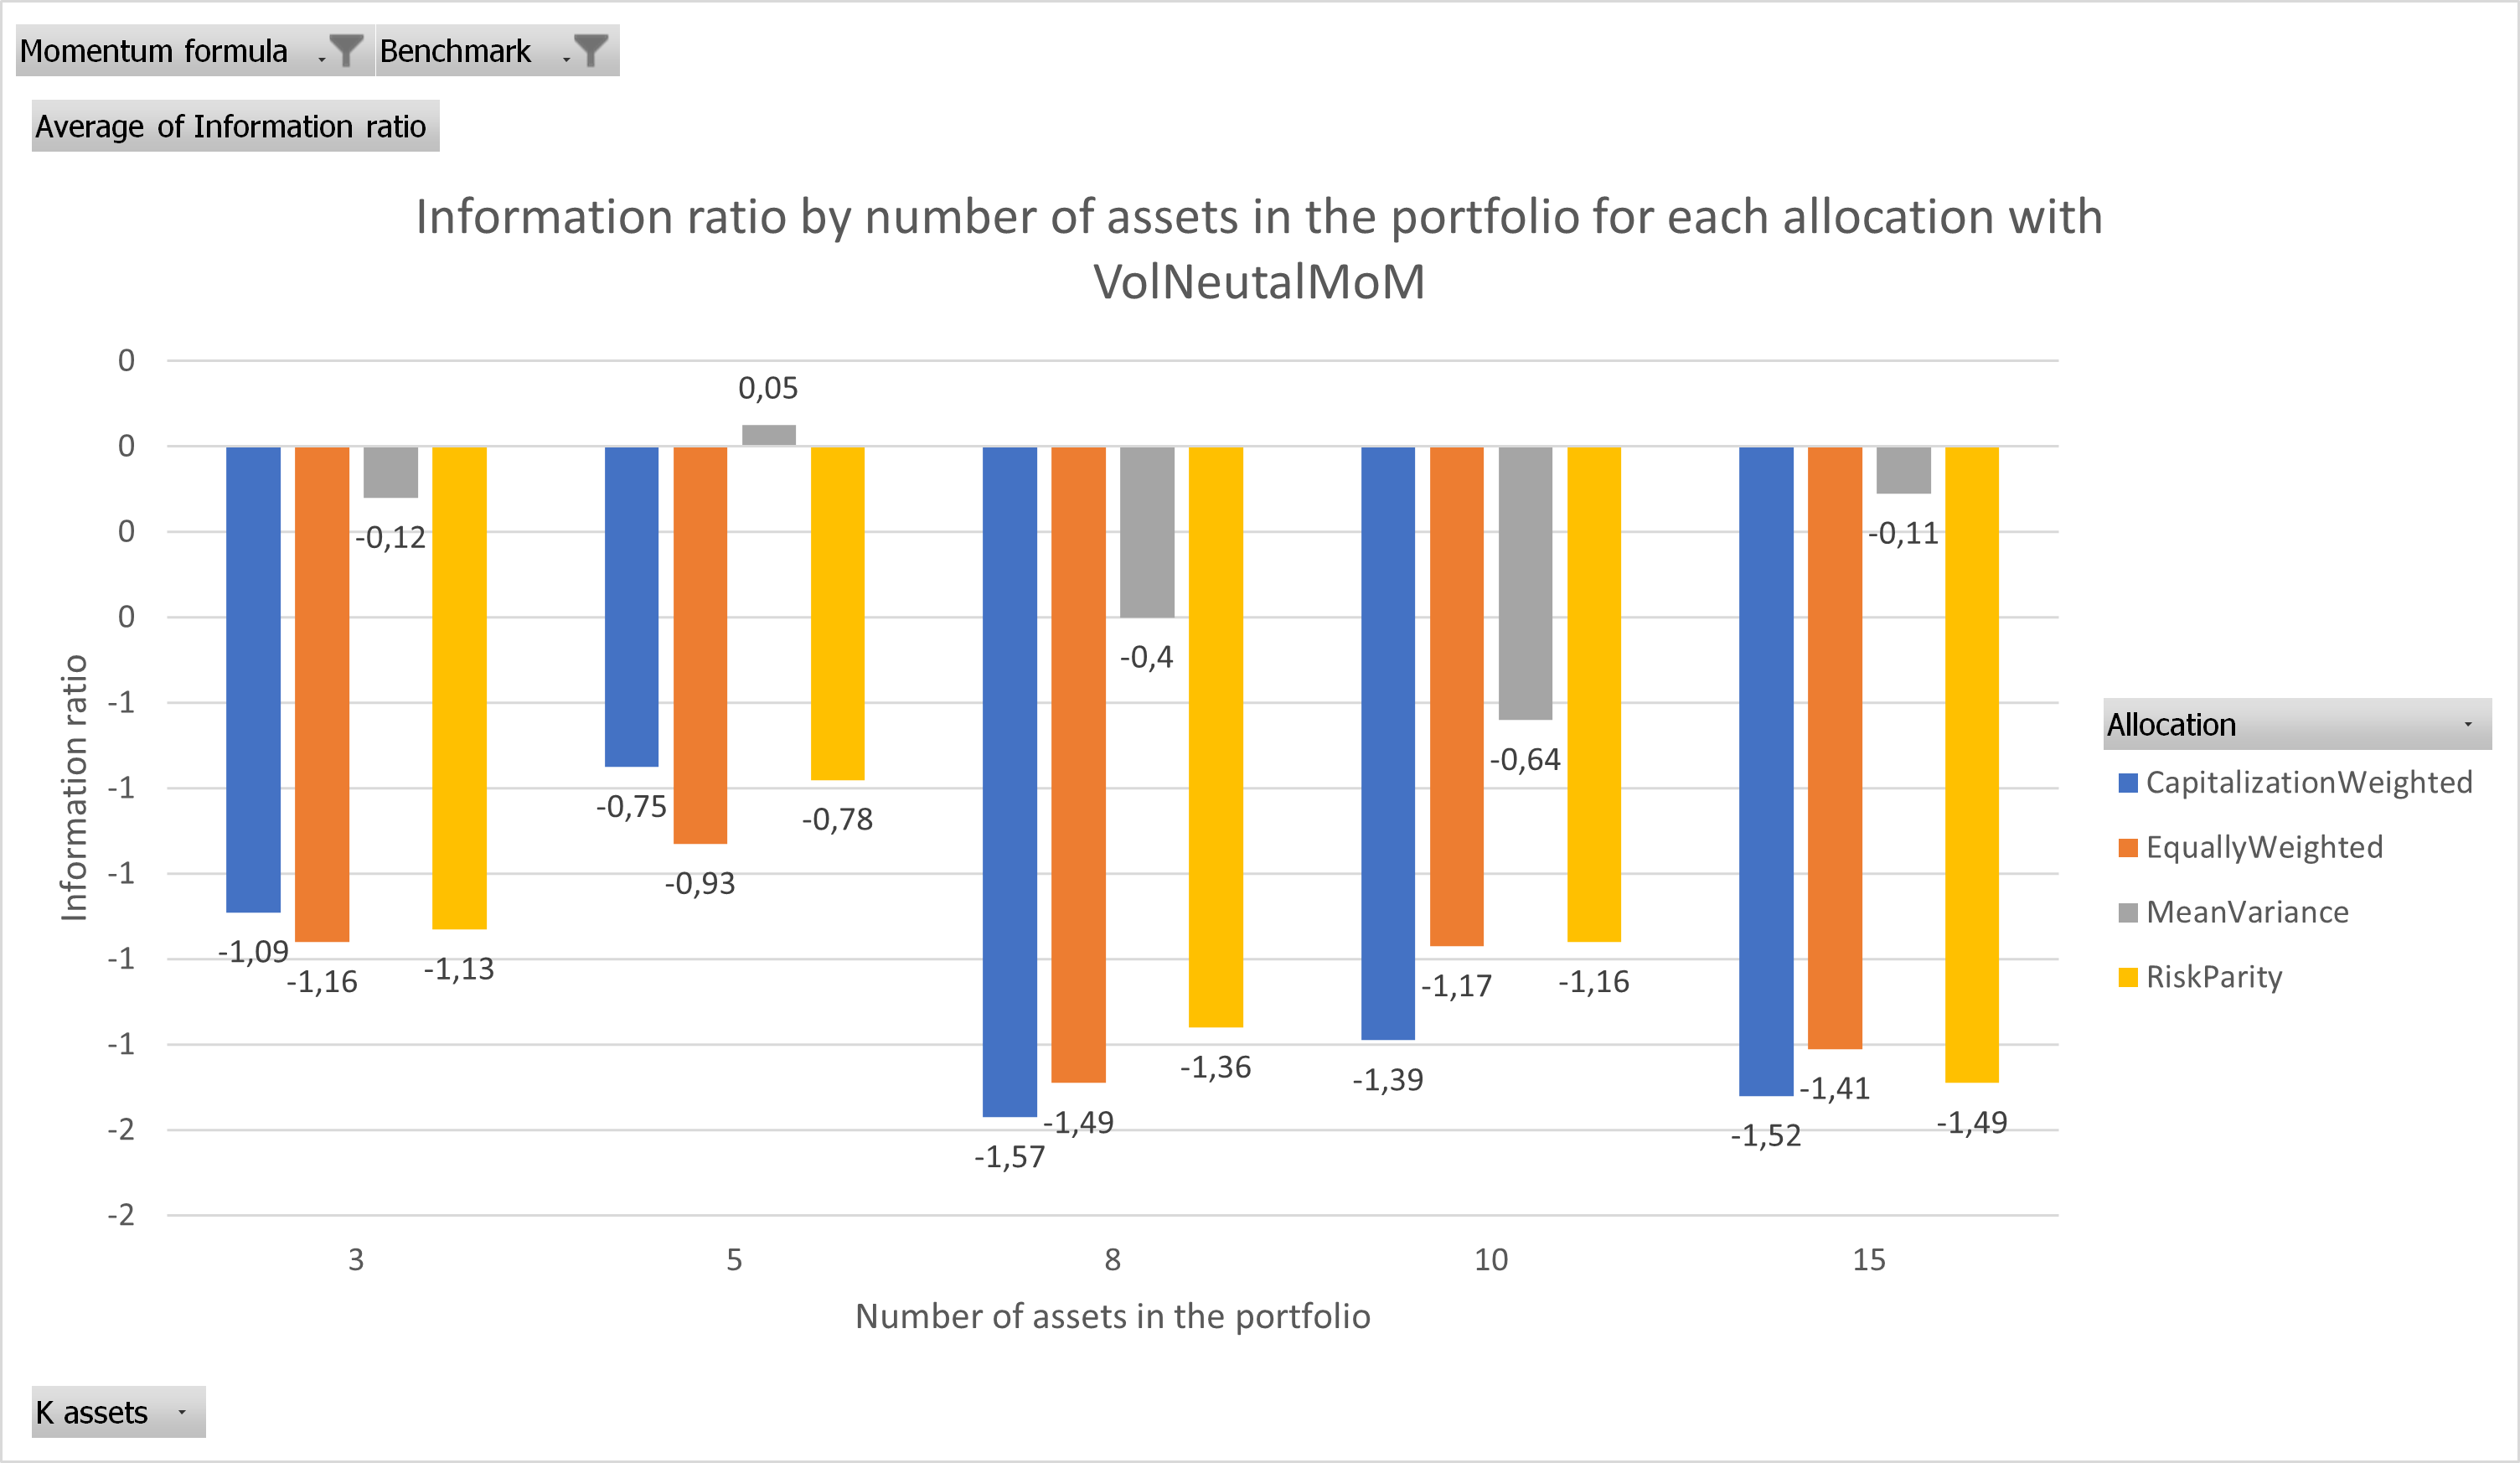
\includegraphics[width=0.75\linewidth]{relative_management/Information ratio VolNeutalMoM_BenchBTC.png}
    \caption{Average Information ratio for each asset allocation method with respect to the number of assets selected in the portfolio for the Volatility Neutral Momentum formula}
    \label{fig:info ratio VolNeutMOM}
\end{figure}

The first thing to notice is that beating the benchmark is very hard even if this benchmark is very risky because of all the idiosyncratic risk included by using a single asset as benchmark.\newline
Across all momentum formula the results are even more consistent than in the previous section \ref{subsubsec:absPtfMngt}. Actually it clear that the mean variance allocation method is still the best suited to beat the benchmark. And the worst allocation method is still the capitalization weighted method. These results confirms the intuition initiated in the previous section \ref{subsubsec:absPtfMngt}. As the momentum strategy is a very aggressive\footnote{When talking about aggressive strategy we could say that they are blend style strategies.} strategy, therefore choosing a conservative asset allocation method reverse the benefit from this strategy.
\newline
Moreover, it is noteworthy that the optimal portfolio size, as evaluated from the perspective of the Information ratio, consistently converges to 5 assets. This observation remains consistent regardless of the specific momentum formula utilized. We attribute this result to the focus of momentum selection on high-performing assets, where an increase in portfolio size raises the likelihood of incorporating underperforming assets. As illustrated in Figure \ref{fig:IRForAllMoM}, the optimal number of assets for risk-adjusted return is found to be less than 8.

Nevertheless, caution must be exercised to avoid an overly low number of assets, as observed in the diversification of idiosyncratic risk and winner volatility, as depicted in Figure \ref{fig:TEForAllMoM}. A balanced portfolio appears to have an optimal number of around 5 assets, considering the need for diversification while acknowledging the heightened tracking error of top-performing assets.


And to conclude on the relative performance from an relative point of view the best performing momentum formula is on average the time series momentum independently from the asset allocation method. We show on the figure \ref{fig:IR_by_aloc_for_all_mom} the average Information ratio no matter the number of asset in the portfolio. 


The significance of the results becomes more pronounced when filtering to retain only 5 assets in the portfolio like in the figure \ref{fig:IR_by_aloc_for_all_mom5assets}. Notably, the Exponential Moving Average (EMA) momentum formula consistently emerges as the least performing among the formulas considered. This observation suggests that the signal generated by the EMA momentum formula may be excessively volatile, limiting its ability to generate substantial positive returns.

\begin{figure}[H] % picture
    \centering
    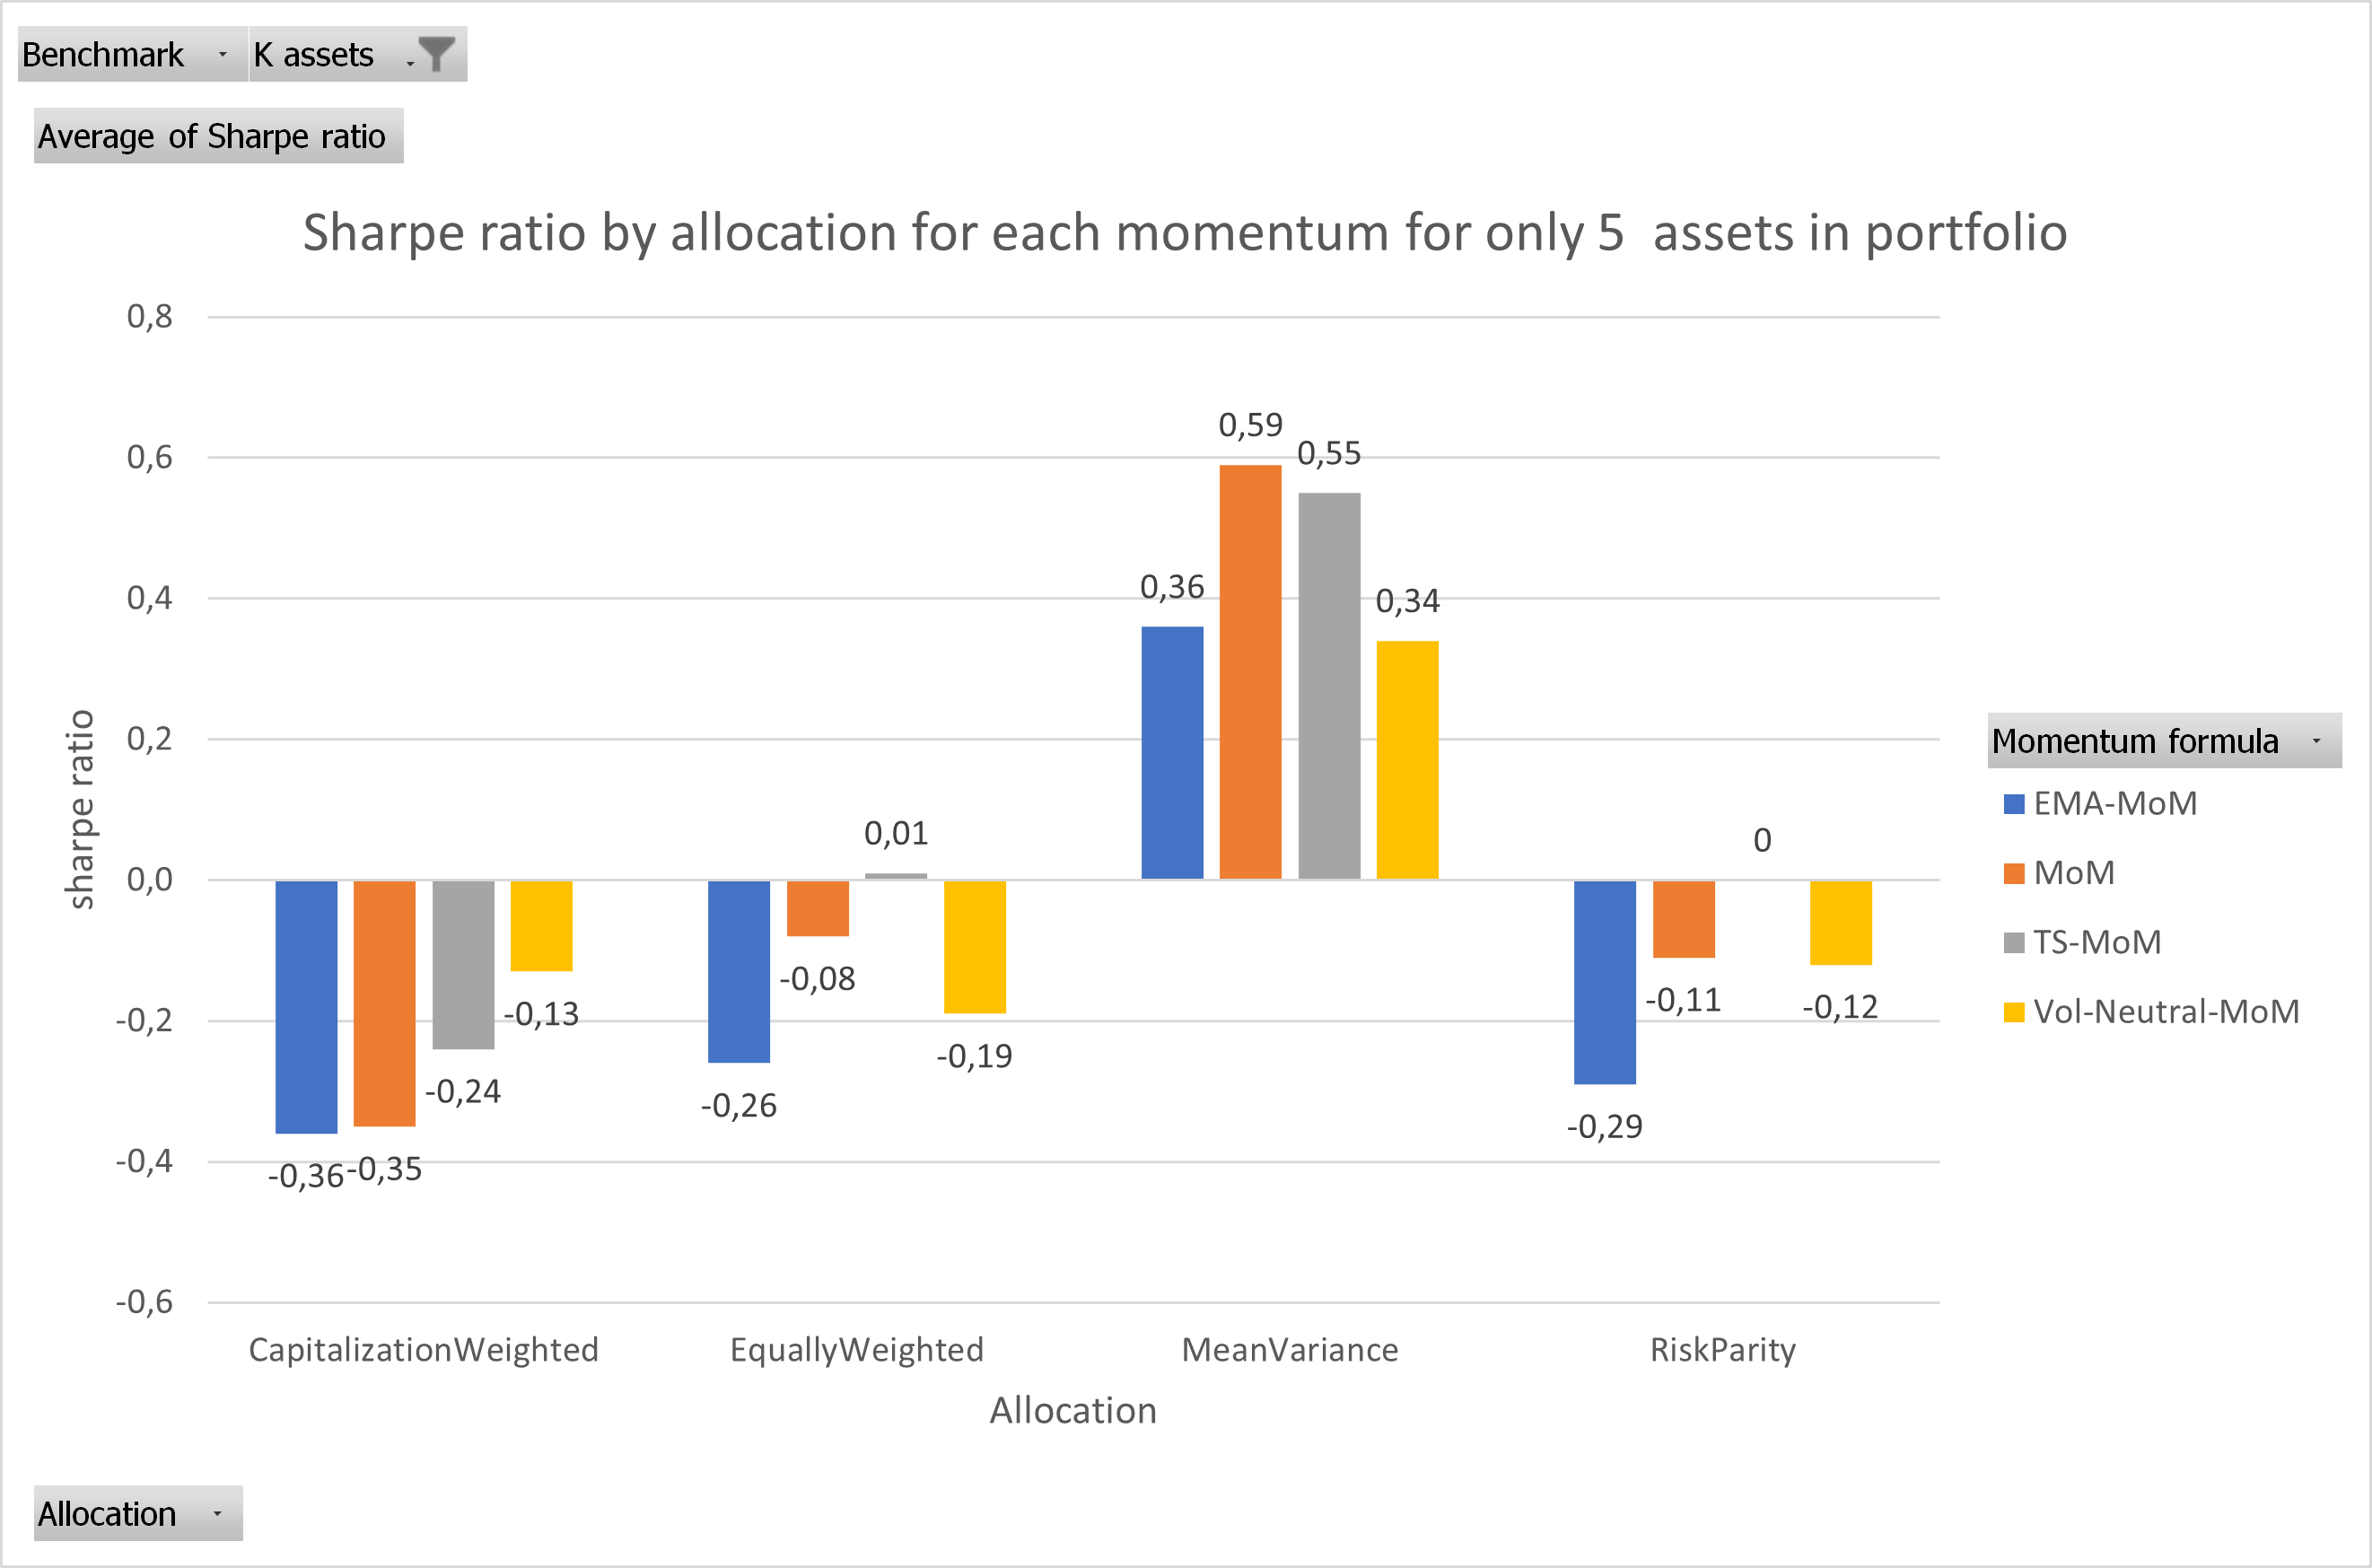
\includegraphics[width=0.75\linewidth]{absolute_management/sharpe_by_aloc_for_all_mom_5_assets.png}
    \caption{Average Information ratio by asset allocation method for each Momentum formula with only 5 assets in the portfolio}
    \label{fig:IR_by_aloc_for_all_mom5assets}
\end{figure}

In conclusion, as detailed in Section \ref{subsec:optimomFSA}, both the relative and absolute performance assessments yield congruent outcomes. The optimal momentum selection formulas are identified as the price momentum by Titman et al. (1993) \cite{Titman1993} and the time series momentum by Moskowitz et al. (2011) \cite{Moskowitz2011}. Notably, within our universe comprising 21 assets, characterized by its relatively modest size, the optimal portfolio size converges to around 5 assets. For a 1-month rebalanced portfolio, the most effective asset allocation method is determined to be the mean-variance approach.

We present below the cumulative performance against the bitcoin and the average return per decile for the portfolio (red) and the benchmark (blue) :

\begin{figure}[H]
   \centering
   \subfloat[Cumulative performances]{
        \label{best_strategy_track}
        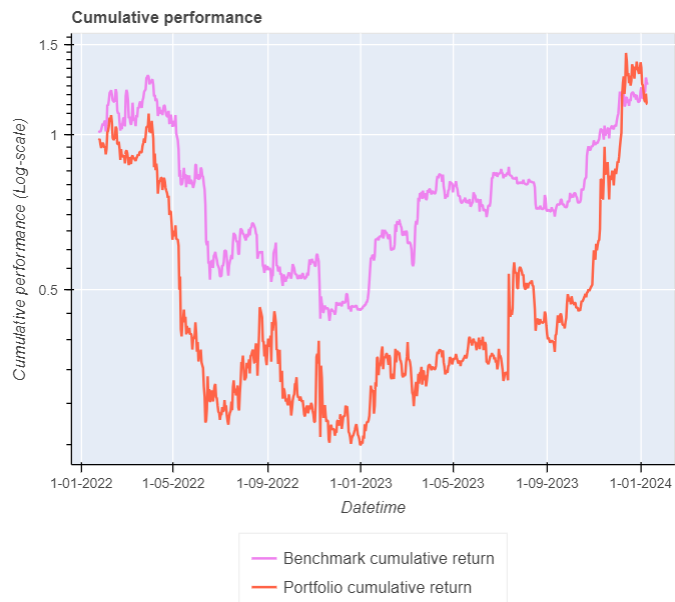
\includegraphics[width=0.5\linewidth]{best_strategy_track.png}
    }
    \subfloat[Returns per decile]{
        \label{best_strategy_decile_perf}
        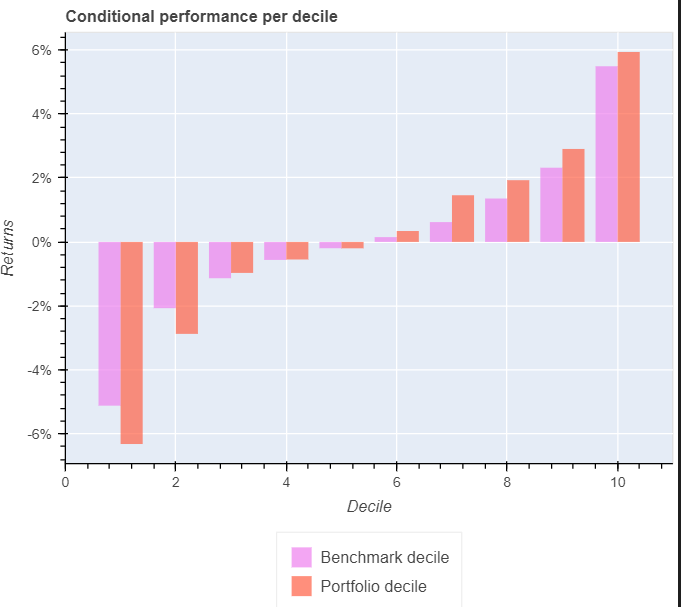
\includegraphics[width=0.5\linewidth]{best_strategy_decile_perf.png}
    }
    \caption{1-month rebalance 172-period Price momentum selection with mean variance allocation against the benchmark.}
    \label{Strategy_plots}
\end{figure}

As demonstrated by the return per decile chart this strategy is very aggressive with respect to the benchmark (BITCOIN). The beta of this strategy is high: 1.10.
\section{Robustness}\label{sec:robustness}
\subsection{Areas of Robustness Testing}
Given the empirical nature of our test, we recognize the importance of conducting robustness checks to validate key aspects of our research. In light of acknowledged data limitations, we have undertaken a thorough examination to address potential issues. The ensuing subsections will underscore the critical points warranting robustness assessment. Specifically, we will focus on validating the selection of optimal momentum periods and confirming the statistical significance of our backtests.

\subsection{Optimal momentum and re-balance period}
To ensure the robustness of our findings, we introduced variability into our analysis by randomly excluding a third of the assets from our universe. Subsequently, we computed the correlation coefficient using the optimal parameters determined in the section \ref{subsec:opt}. The obtained coefficients from this randomly altered universe were then compared with those calculated using the entire dataset.

\begin{figure}[H] % picture
    \centering
    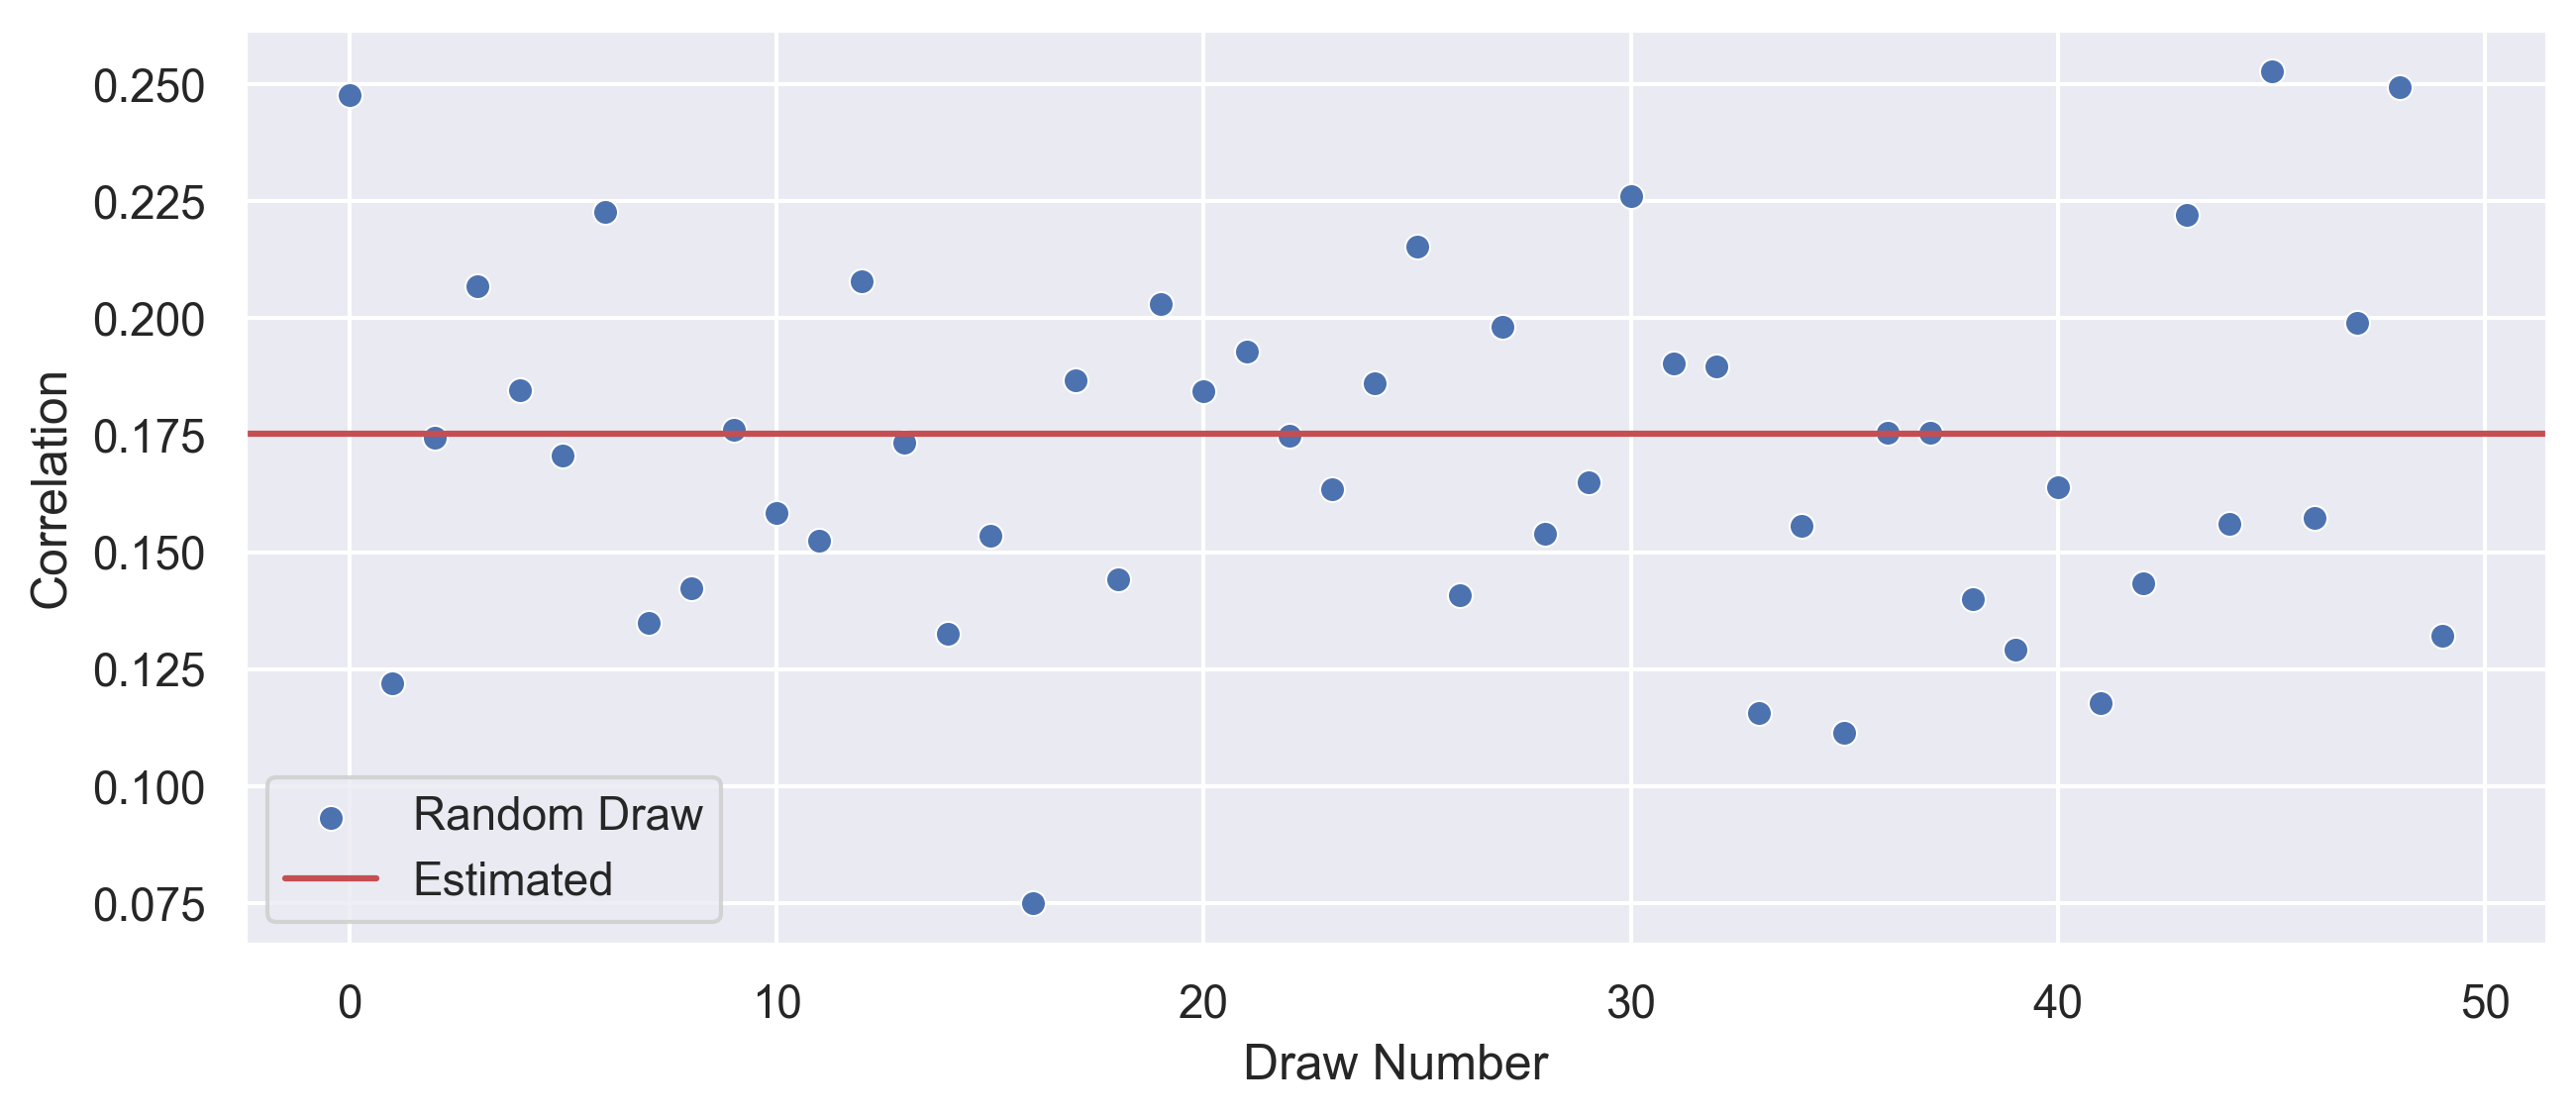
\includegraphics[width=1\linewidth]{robustness.png}
    \caption{Correlation outcomes with a randomly altered universe}
    \label{fig:fig3}
\end{figure}

\paragraph{}
Despite the observed dispersion, it is noteworthy that the correlation we previously derived does not exhibit signs of overfitting, as the correlations obtained with the randomly altered universe are not notably lower.

\subsection{Ensuring Statistical Significance in Backtests}
In our backtests, we identified a potential risk associated with random exposure to the benchmark when allocating for a long portfolio. Given that our portfolio is long-only in certain backtests, it is crucial to ascertain that our results exhibit statistical differences from the benchmark. This verification is essential to confirm that our strategy indeed provides exposure distinct from that of the benchmark.

To address this concern, we employed a bootstrapping method involving random sampling from our backtest results. Various metrics such as Sharpe ratio, Expected Returns, Volatility, VaR, CVaR, among others \ref{subsec:perfandrisk}, were computed based on these samples. Subsequently, we assessed whether these metrics demonstrated statistical differences from those of the benchmark. Across all the presented backtests in this paper, our analysis consistently reveals that the metrics of our strategy are significantly different from those of the benchmark with a confidence level exceeding 99\%. This leads us to the conclusion that our momentum strategies not only avoid mirroring the cryptocurrency market but also exhibit statistically distinct inherent exposures.

\section{Conclusion}

In this comprehensive study, we have explored the intricate dynamics of momentum-based portfolio management, delving into both absolute and relative performance frameworks. Our analysis encompasses various momentum formulas, asset allocation methods, and portfolio sizes, providing a nuanced understanding of their collective impact on portfolio performance.

\paragraph{Optimal Momentum and Re-balance Period}

The optimization of lookback and horizon periods further refines our approach, emphasizing the delicate balance between exploiting momentum effects and avoiding overfitting. The derived optimal combination of a 519-day lookback and 30-day horizon underscores the persistent nature of returns within these timeframes.

\paragraph{Absolute Portfolio Management}

Our investigation into absolute portfolio management styles highlights the significance of selecting an appropriate asset allocation method and momentum formula. The mean-variance approach consistently emerges as the optimal choice, demonstrating superior risk-adjusted returns. Equally weighted and risk parity approaches, despite their simplicity, fall short of capturing the full potential of momentum strategies.\newline

The observed optimal portfolio size, around 5 assets, underscores the delicate balance required for effective risk management and performance enhancement. Notably, the time series momentum formula consistently outperforms other formulations across various asset allocation methods and portfolio sizes. Additionally, caution is warranted to avoid an overly low number of assets, as excessive concentration may compromise diversification benefits.\newline

The robustness testing further validates the statistical significance of our findings, confirming the distinct exposure of our momentum strategies compared to the benchmark. Our methodology incorporates bootstrapping methods and thorough robustness checks, affirming the reliability of our conclusions.\newline

\paragraph{Relative Portfolio Management}
In the realm of relative portfolio management, our analysis extends the insights gained from absolute performance. The mean-variance approach, once again, emerges as the most effective asset allocation method, surpassing capitalization-weighted and equally weighted methods. The optimal portfolio size, consistent at around 5 assets, reinforces the importance of balancing diversification and relative risk-adjusted returns.\newline

The time series momentum formula remains the top-performer in relative portfolio management, aligning with its absolute performance. Beating the benchmark, though challenging, is consistently achieved with the mean-variance approach.\newline

Our robustness testing extends to the relative performance domain, confirming statistical differences from the benchmark and reaffirming the distinctive exposure of our strategies. We tried to maintain 
a low level of overfitting through our research.\newline


In conclusion, our comprehensive analysis demonstrates the effectiveness of momentum-based strategies in both absolute and relative portfolio management. The careful selection of asset allocation methods, momentum formulas, and optimal periods is crucial for maximizing returns and managing risk. The findings of this study offer valuable insights for practitioners and researchers in navigating the complex landscape of momentum-based portfolio management.
In subsequent stages of research, it would be beneficial to investigate the dynamic evolution of asset weights within the portfolio. Analyzing the consistency, seasonality, and persistence of these weights could provide valuable insights into optimal portfolio management.

Exploring advanced modeling techniques, such as Gaussian Mixture or Hidden Markov Models, to characterize market regimes and determine optimal tactical allocations under different market conditions could further enhance our understanding.

The introduction of a skewness risk allocation, as proposed by Lezmi et al. (2018) \cite{lezmi2018portfolio}, has the potential to refine the allocation method. Given the mean-reverting nature and skewed returns of cryptocurrency prices, incorporating this allocation approach may yield unexpected yet insightful outcomes.

Additionally, assessing the efficiency of the cryptocurrency market through statistical tests, as suggested by Garcin et al. (2022) \cite{brouty2022statistical}, would be a crucial step in evaluating the market dynamics and refining our portfolio management strategies.

\bibliography{references}
\bibliographystyle{unsrt}
\section{Appendix}\label{sec:appendix}
\subsection{Images}

\begin{figure}[H] % picture
    \centering
    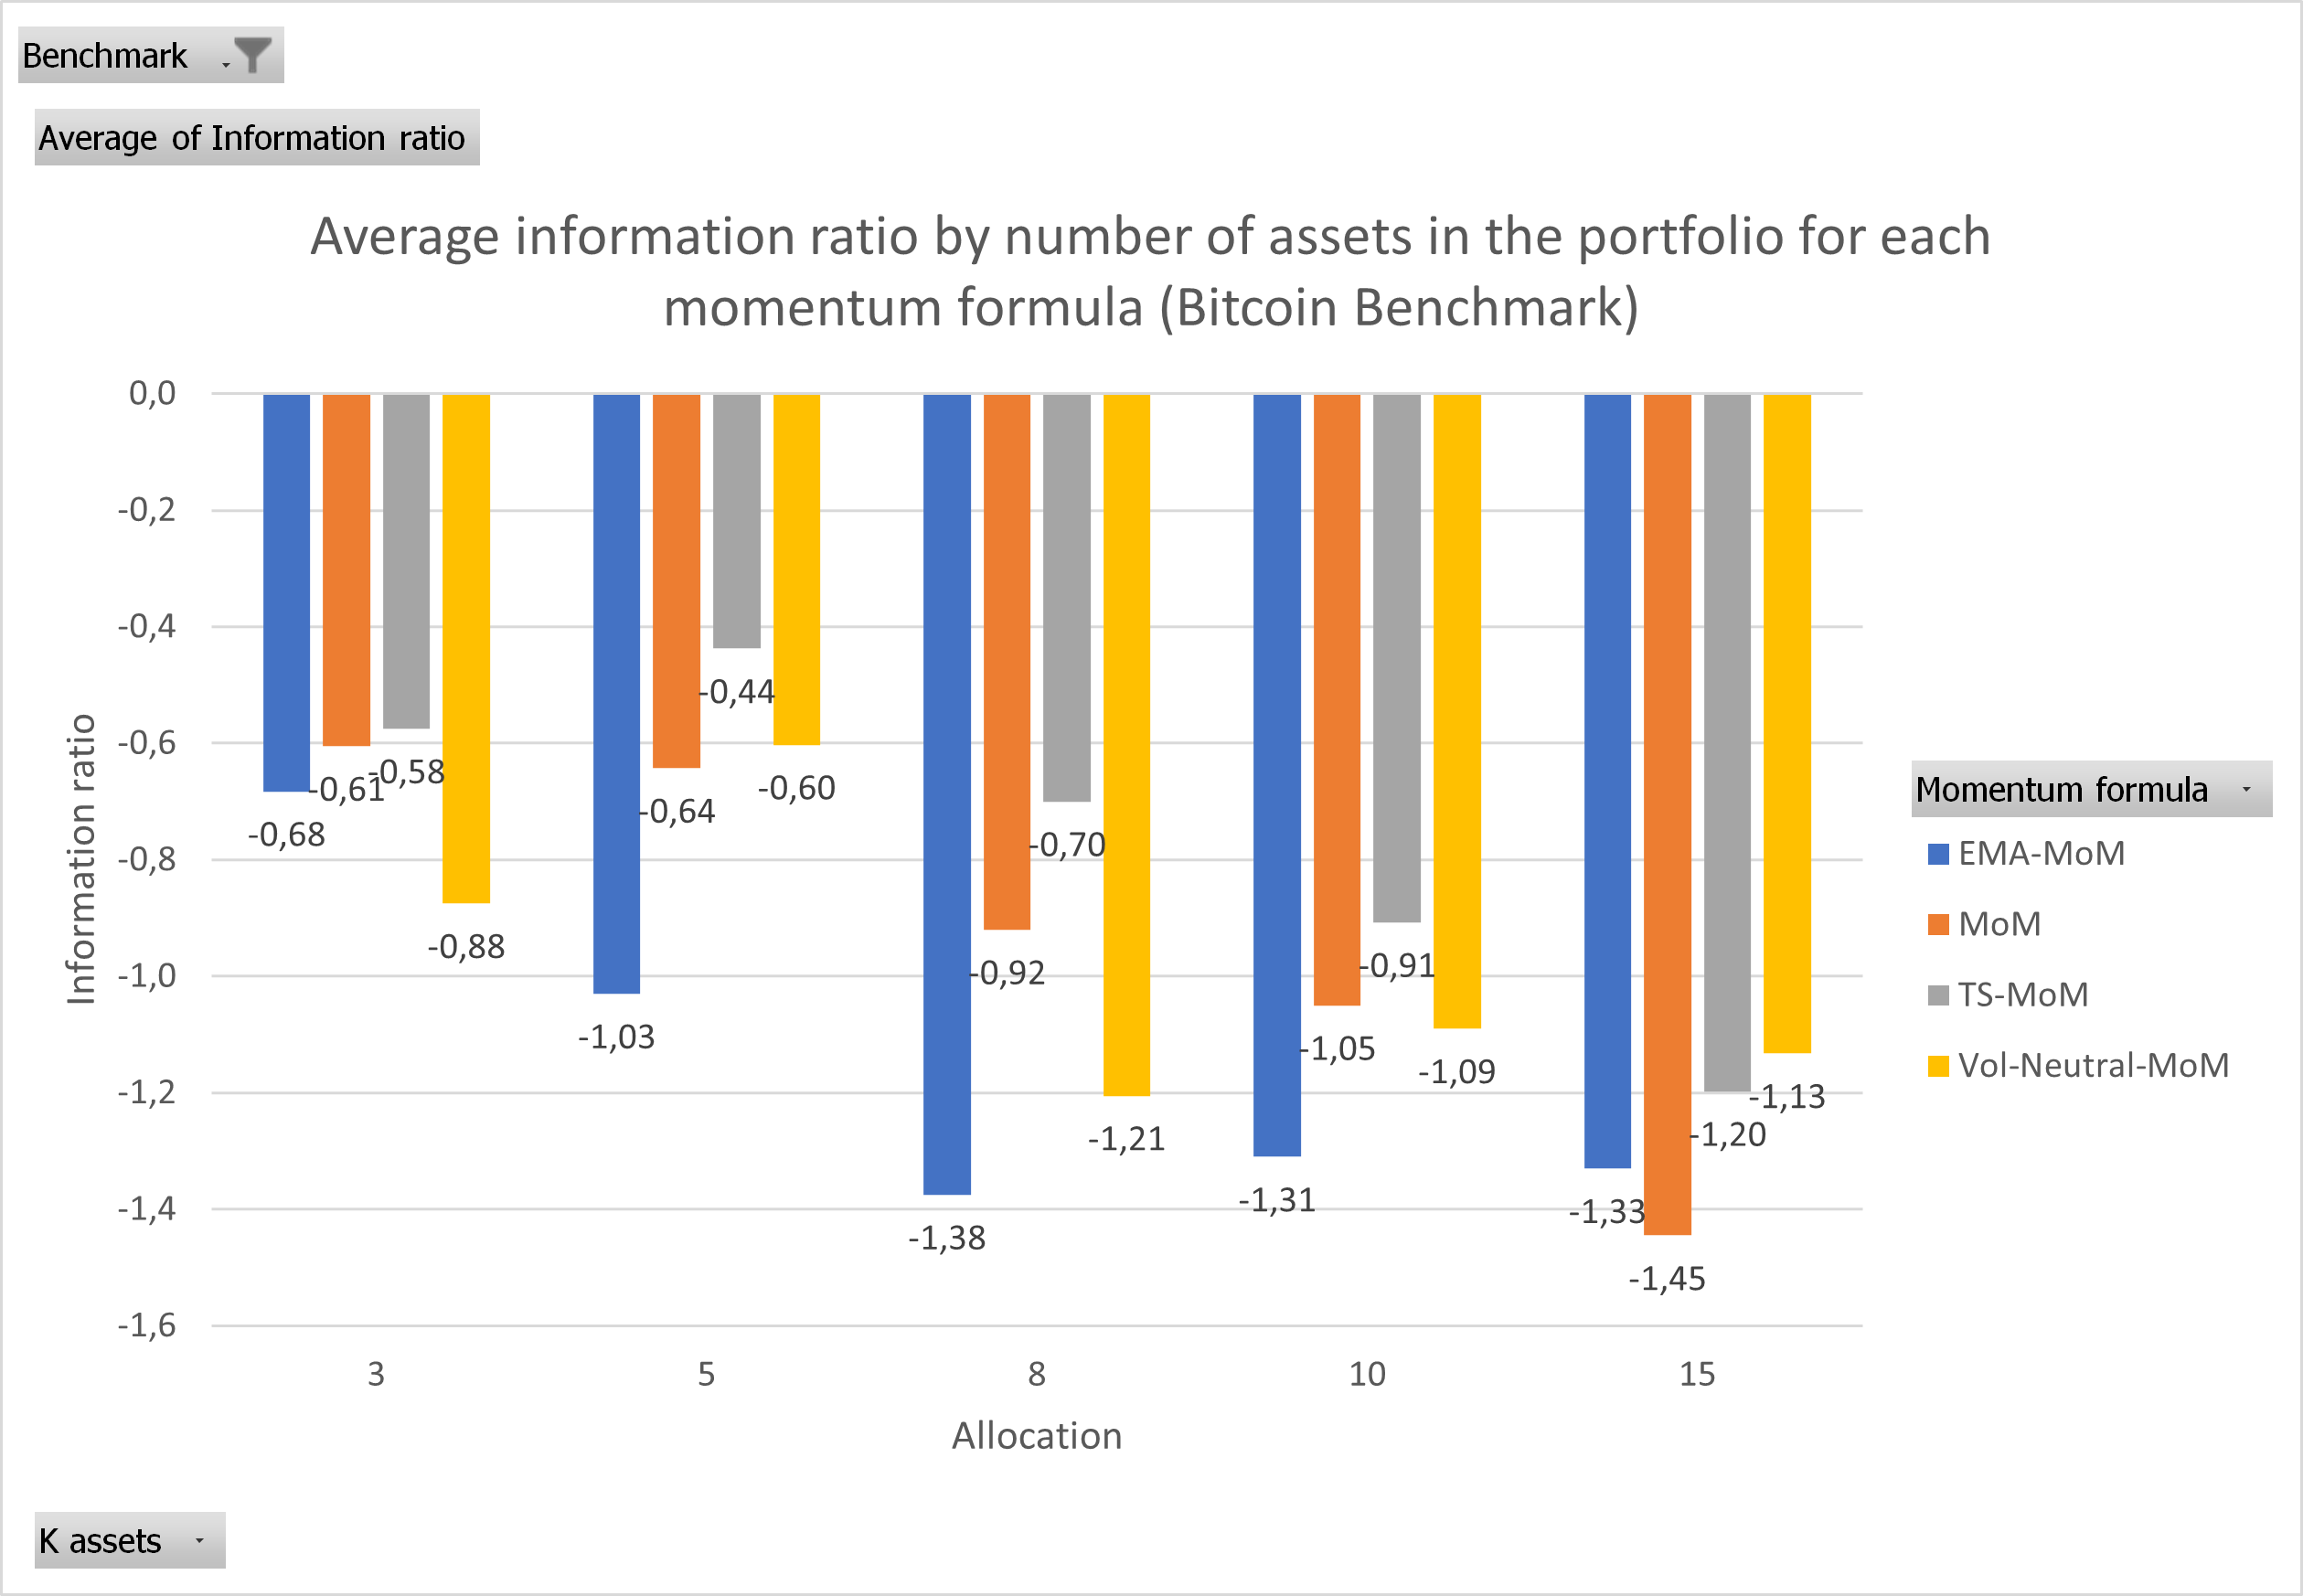
\includegraphics[width=0.75\linewidth]{relative_management/btc_bench_IR_by_k_assets_for_formula.png}
    \caption{Average Information ratio for each Momentum formula concerning the number of assets selected in the portfolio}
    \label{fig:IRForAllMoM}
\end{figure}

\begin{figure}[H] % picture
    \centering
    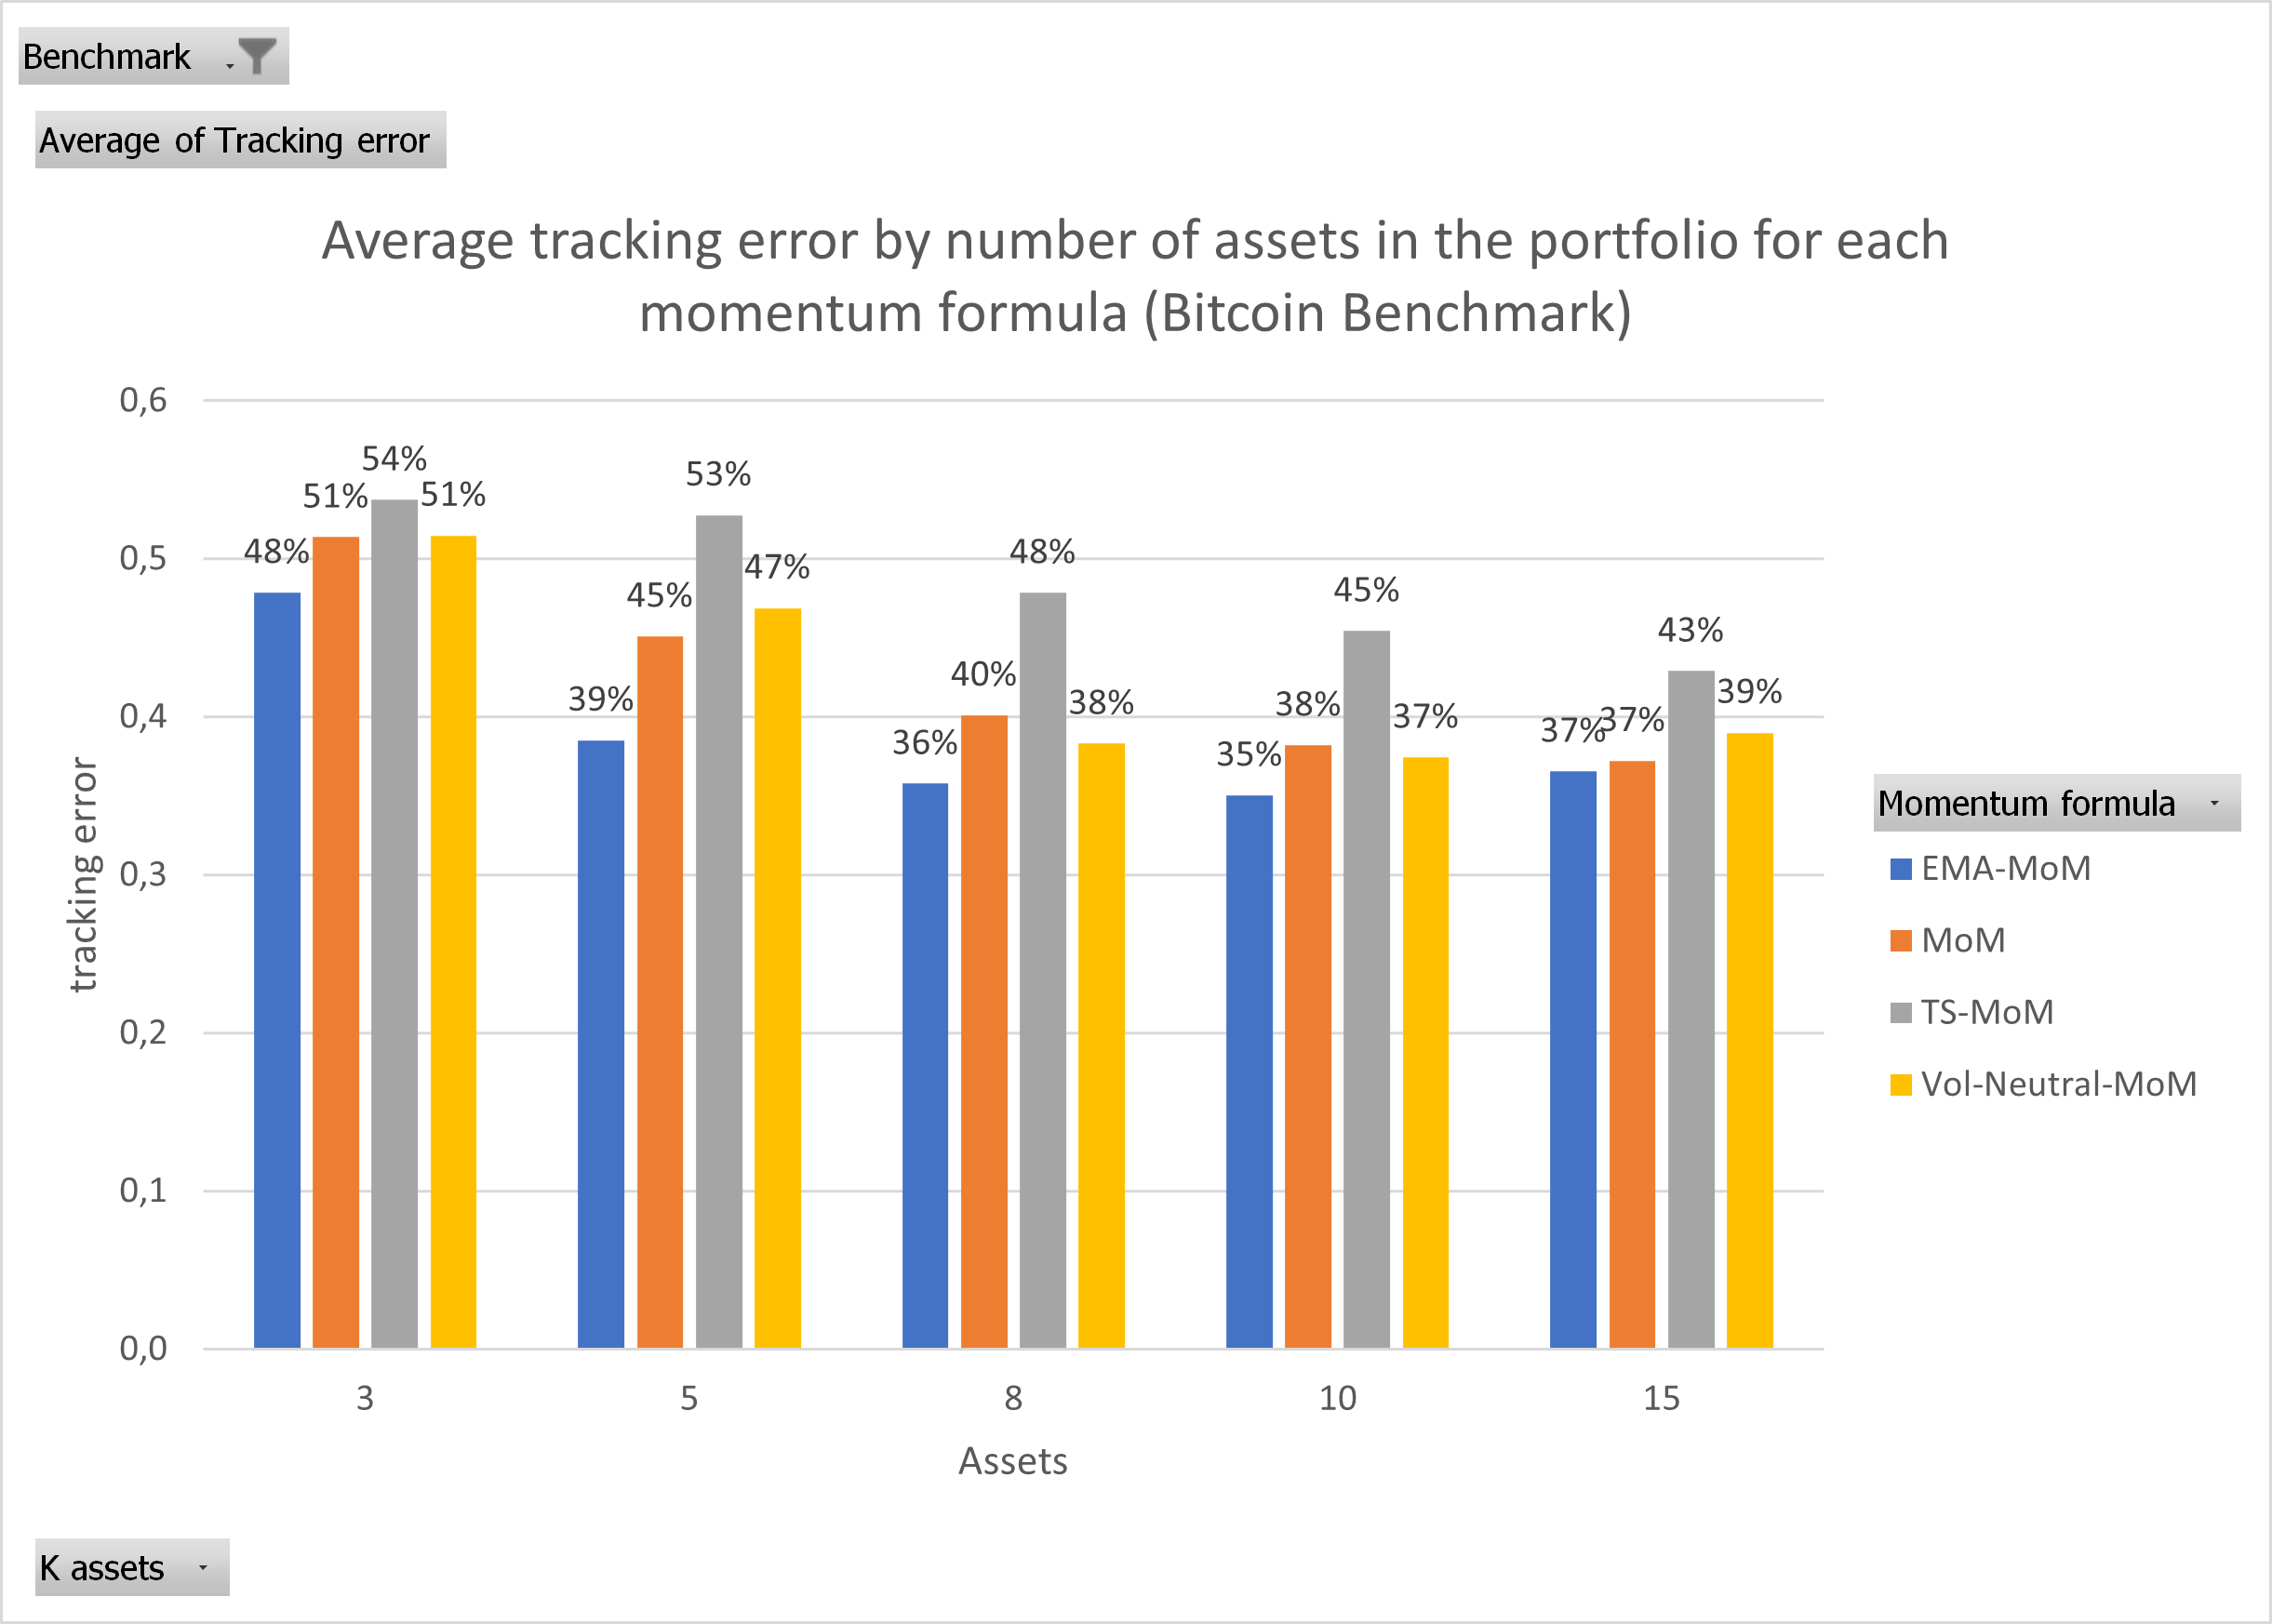
\includegraphics[width=0.75\linewidth]{relative_management/btc_bench_TE_by_k_assets_for_formula.png}
    \caption{Average Tracking Error for each Momentum formula concerning the number of assets selected in the portfolio}
    \label{fig:TEForAllMoM}
\end{figure}
\begin{figure}[H] % picture
    \centering
    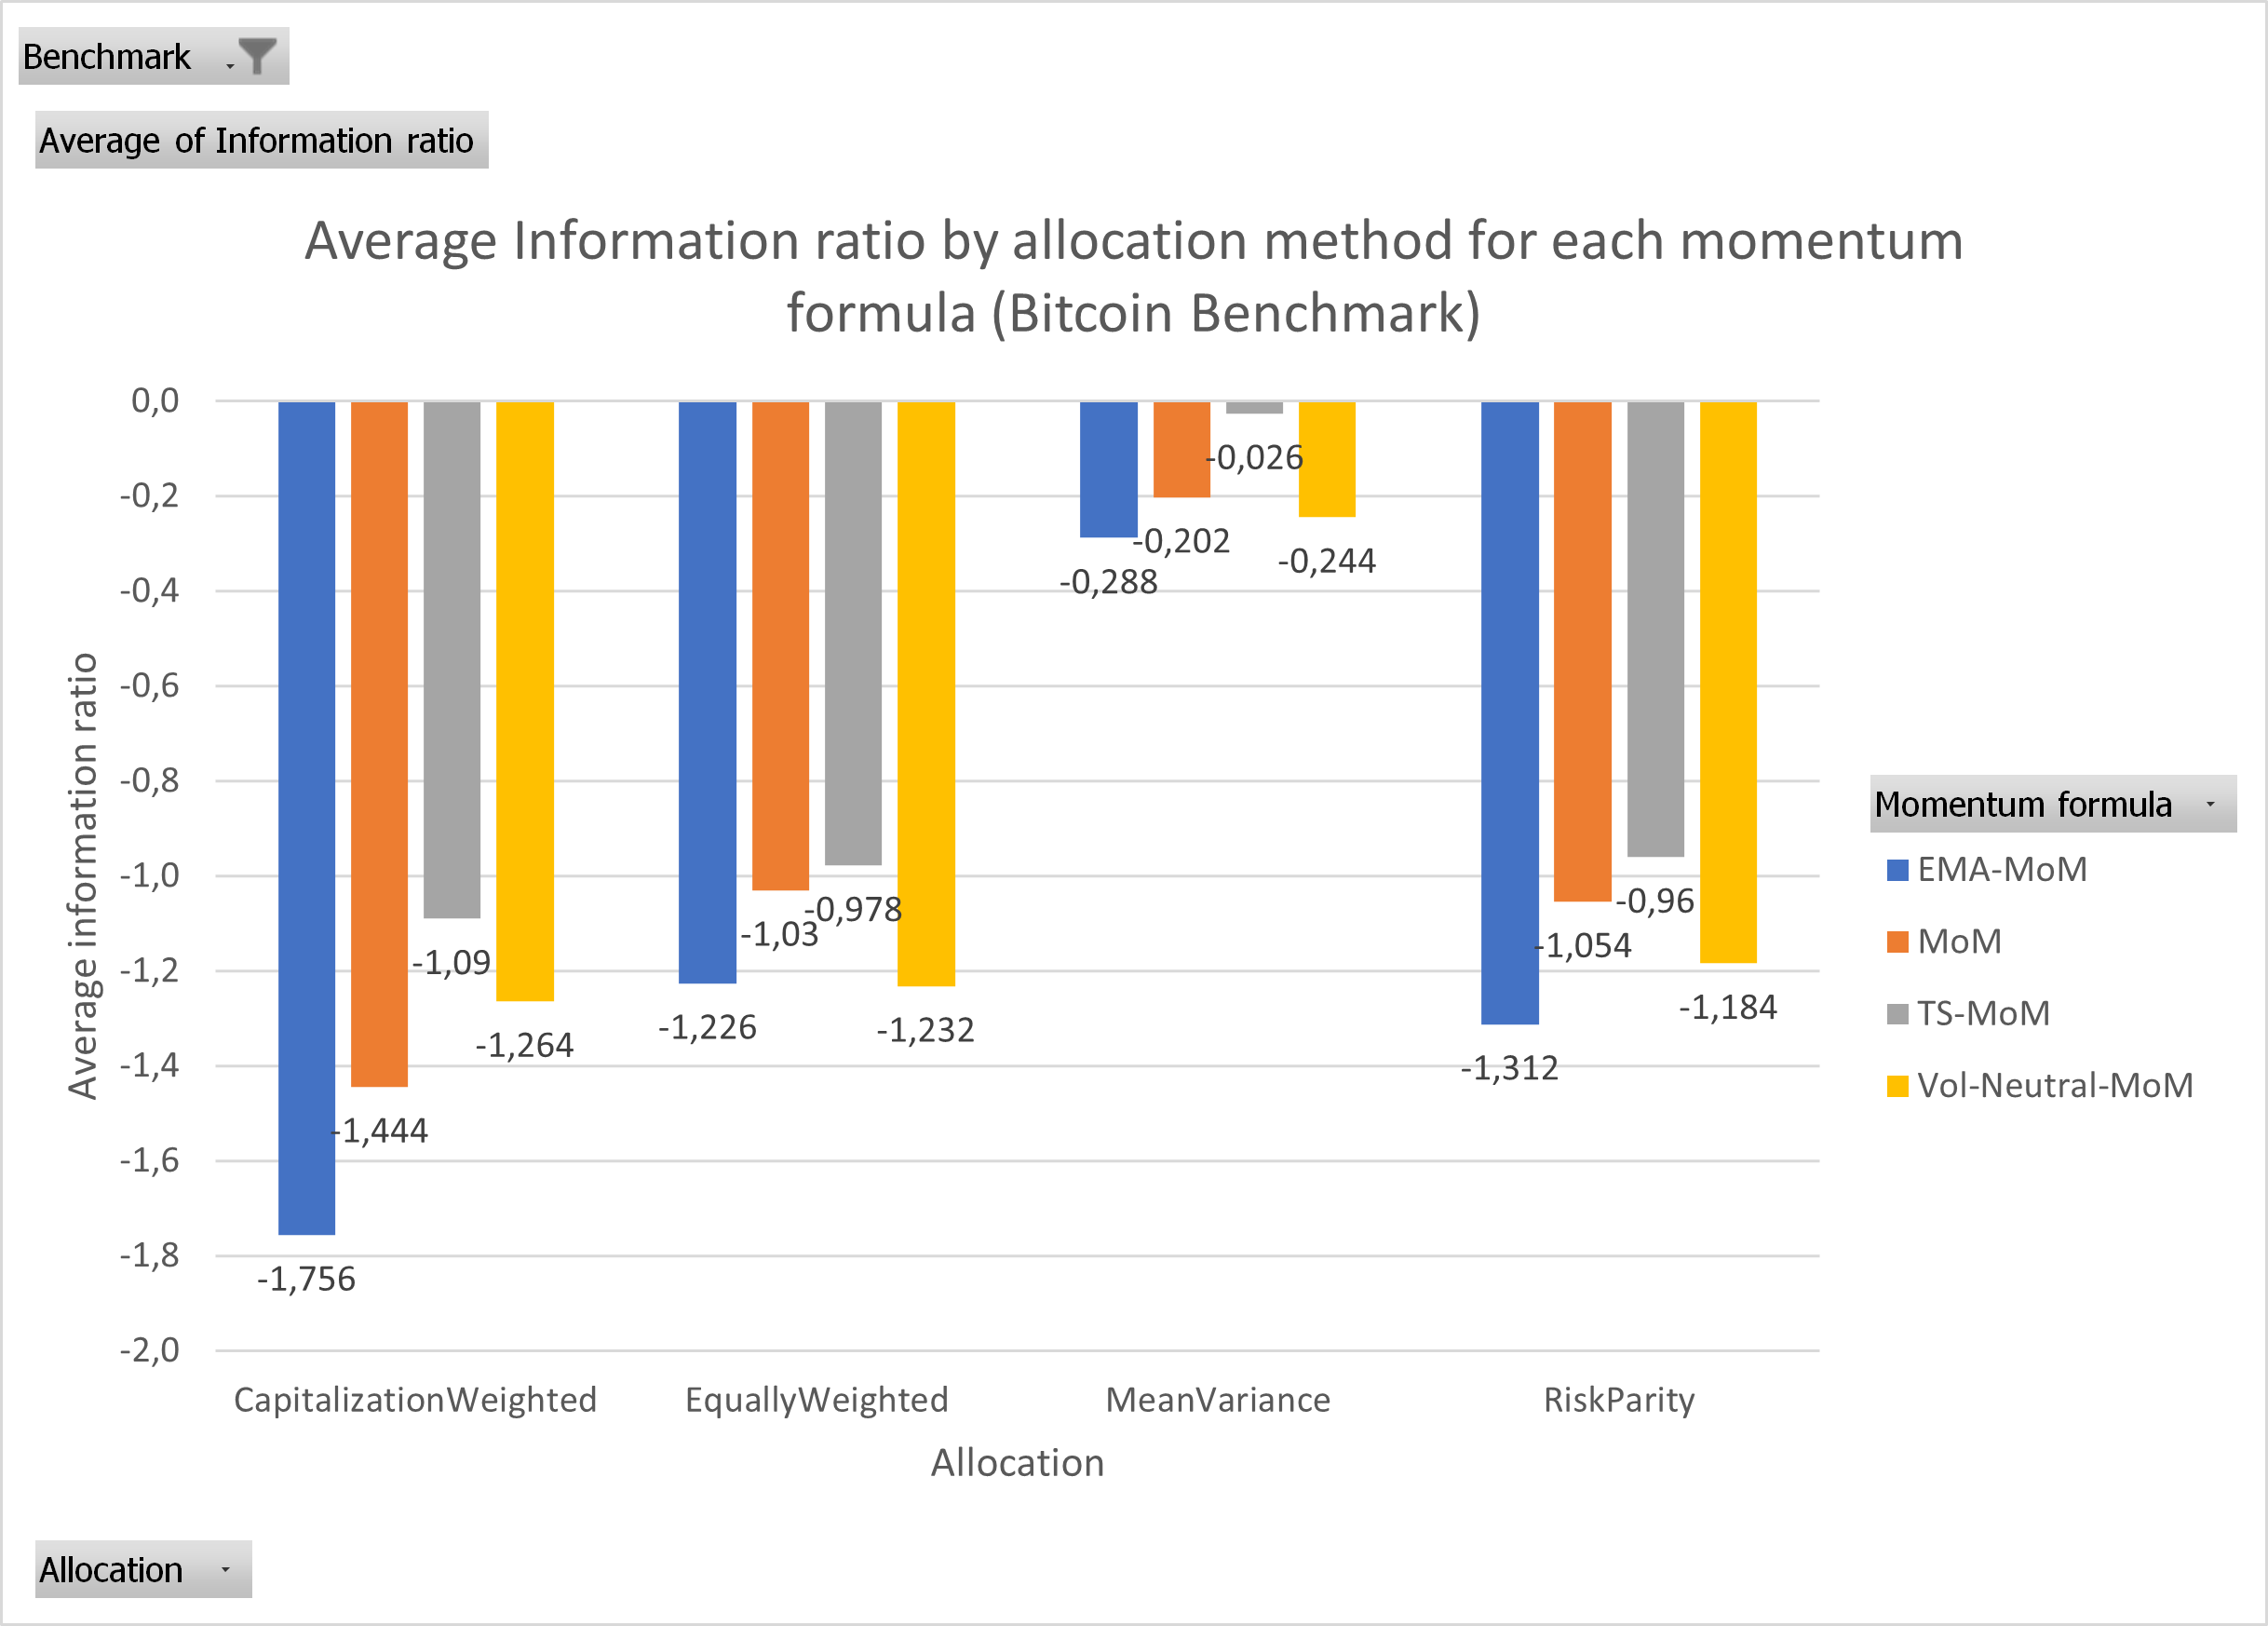
\includegraphics[width=0.75\linewidth]{relative_management/IR_by_aloc_for_all_mom.png}
    \caption{Average Information ratio by asset allocation method for each Momentum formula}
    \label{fig:IR_by_aloc_for_all_mom}
\end{figure}
\subsection{Tables}
\begin{table}[H]
    \centering
    \caption{List of Cryptocurrency Pairs}
    \label{tab:crypto_pairs}
    \begin{tabular}{|c|}
        \hline
        \textbf{Cryptocurrency Pairs} \\
        \hline
        BTC-USDT \\
        MATIC-USDT \\
        LTC-USDT \\
        ADA-USDT \\
        XLM-USDT \\
        ATOM-USDT \\
        XRP-USDT \\
        XTZ-USDT \\
        ETC-USDT \\
        DOGE-USDT \\
        ETH-USDT \\
        SOL-USDT \\
        VET-USDT \\
        LINK-USDT \\
        DASH-USDT \\
        BCH-USDT \\
        KDA-USDT \\
        BNB-USDT \\
        EOS-USDT \\
        TRX-USDT \\
        AVAX-USDT \\
        \hline
    \end{tabular}
\end{table}
\begin{landscape}
\begin{table}[H]
  \centering
  \begin{tabular}{p{0.4cm}|p{3cm}|p{1.65cm}|p{1.65cm}|p{1.65cm}|p{1.65cm}|p{1.65cm}|p{1.65cm}|p{1.65cm}|p{1.65cm}|p{1.65cm}}%{lllllllllll}
    \toprule
    \multicolumn{2}{c}{Assets \& Benchmarks}                   \\
    \cmidrule(r){1-2}
    $k$ & benchmark & CVaR & Expected return & Expected volatility&Information ratio&Portfolio beta&Sharpe ratio&Tail ratio&Tracking error&VaR\\
    \midrule
    3&BITCOIN&-8.53\% (-9.49)&-20.54\% (-4.32)&68.59\% (13.10)&-1.13 (-7.42)&1.01 (0.16)&-0.30 (-5.00)&0.95 (-1.26)&40.46\% (54.48)&-6.11\% (-13.92)
\\ 
3&CAPITALIZATION WEIGHTED&-8.53\% (-2.05)&-20.54\% (-2.14)&68.59\% (4.99)&-0.46 (-4.91)&0.98 (-3.55)&-0.30 (-2.35)&0.95 (1.43)&31.11\% (69.19)&-6.11\% (-5.66)
\\ 
3&EQUAL WEIGHTED&-8.53\% (3.73)&-20.54\% (-0.45)&68.59\% (-1.54)&-0.10 (-0.82)&0.90 (-12.49)&-0.30 (-0.53)&0.95 (3.77)&30.57\% (98.76)&-6.11\% (5.98)
\\ 
5&BITCOIN&-8.60\% (-9.59)&-8.83\% (-2.49)&72.28\% (12.50)&-0.78 (-6.56)&1.06 (5.59)&-0.12 (-3.92)&0.99 (0.77)&43.52\% (29.94)&-6.05\% (-18.43)
\\ 
5&CAPITALIZATION WEIGHTED&-8.60\% (-2.54)&-8.83\% (0.32)&72.28\% (5.96)&-0.09 (-2.49)&1.04 (3.35)&-0.12 (0.09)&0.99 (1.83)&31.22\% (28.88)&-6.05\% (-5.67)
\\ 
5&EQUAL WEIGHTED&-8.60\% (5.63)&-8.83\% (1.83)&72.28\% (2.02)&0.30 (0.63)&0.97 (-2.89)&-0.12 (1.39)&0.99 (5.28)&28.85\% (30.81)&-6.05\% (5.03)
\\ 
8&BITCOIN&-8.57\% (-9.49)&-25.45\% (-3.86)&68.66\% (13.13)&-1.36 (-8.84)&1.06 (6.71)&-0.37 (-4.22)&0.92 (-3.36)&37.13\% (40.39)&-6.06\% (-13.49)
\\ 
8&CAPITALIZATION WEIGHTED&-8.57\% (-2.24)&-25.45\% (-1.09)&68.66\% (6.05)&-0.84 (-5.54)&1.03 (5.55)&-0.37 (-1.29)&0.92 (1.61)&23.03\% (35.83)&-6.06\% (-5.30)
\\ 
8&EQUAL WEIGHTED&-8.57\% (3.46)&-25.45\% (-0.32)&68.66\% (0.87)&-0.41 (-2.20)&0.96 (-6.65)&-0.37 (-0.60)&0.92 (4.82)&18.98\% (31.44)&-6.06\% (5.08)
\\ 
10&BITCOIN&-8.73\% (-10.42)&-17.34\% (-3.62)&69.31\% (13.51)&-1.16 (-7.18)&1.08 (8.93)&-0.25 (-4.34)&0.93 (-2.45)&36.44\% (45.54)&-6.06\% (-12.69)
\\ 
10&CAPITALIZATION WEIGHTED&-8.73\% (-3.65)&-17.34\% (-1.48)&69.31\% (6.48)&-0.52 (-4.86)&1.05 (9.15)&-0.25 (-1.46)&0.93 (0.39)&21.42\% (47.13)&-6.06\% (-6.18)
\\ 
10&EQUAL WEIGHTED&-8.73\% (3.88)&-17.34\% (-0.37)&69.31\% (-0.46)&0.02 (-1.36)&0.99 (-5.38)&-0.25 (-0.49)&0.93 (4.07)&14.79\% (39.14)&-6.06\% (5.33)
\\ 
15&BITCOIN&-9.17\% (-12.47)&-30.47\% (-6.78)&70.32\% (20.50)&-1.49 (-10.80)&1.09 (8.26)&-0.43 (-7.11)&0.86 (-7.32)&37.11\% (77.70)&-6.52\% (-18.70)
\\ 
15&CAPITALIZATION WEIGHTED&-9.17\% (-6.11)&-30.47\% (-1.16)&70.32\% (8.98)&-1.18 (-6.79)&1.08 (12.90)&-0.43 (-1.12)&0.86 (-1.23)&20.60\% (75.77)&-6.52\% (-6.71)
\\ 
15&EQUAL WEIGHTED&-9.17\% (1.71)&-30.47\% (1.18)&70.32\% (1.69)&-1.39 (-7.53)&1.01 (6.63)&-0.43 (1.39)&0.86 (3.50)&9.27\% (70.53)&-6.52\% (2.65)
\\
    \bottomrule
  \end{tabular}
  \label{tab:volneutmom172riskparity}
   \caption{Performance \& risks from the backtest for the 172 periods Volatility Neutral Momentum. The underlying strategy uses a risk parity allocation and is rebalanced monthly.}
\end{table}
\end{landscape}
\begin{landscape}
\begin{table}[H]
  \centering
  \begin{tabular}{p{0.4cm}|p{3cm}|p{1.65cm}|p{1.65cm}|p{1.65cm}|p{1.65cm}|p{1.65cm}|p{1.65cm}|p{1.65cm}|p{1.65cm}|p{1.65cm}}%{lllllllllll}
    \toprule
    \multicolumn{2}{c}{Assets \& Benchmarks}                   \\
    \cmidrule(r){1-2}
    $k$ & benchmark & CVaR & Expected return & Expected volatility&Information ratio&Portfolio beta&Sharpe ratio&Tail ratio&Tracking error&VaR\\
    \midrule
    3&BITCOIN&-8.88\% (-10.97)&-23.53\% (-3.05)&71.48\% (16.19)&-1.16 (-5.73)&1.06 (5.61)&-0.33 (-3.86)&0.94 (-0.63)&41.92\% (54.50)&-6.50\% (-14.53)
\\ 
3&CAPITALIZATION WEIGHTED&-8.88\% (-3.27)&-23.53\% (-1.50)&71.48\% (8.55)&-0.56 (-4.00)&1.03 (3.13)&-0.33 (-1.44)&0.94 (2.38)&31.24\% (70.43)&-6.50\% (-6.97)
\\ 
3&EQUAL WEIGHTED&-8.88\% (0.10)&-23.53\% (-1.70)&71.48\% (1.76)&-0.19 (-4.18)&0.94 (-8.63)&-0.33 (-1.82)&0.94 (1.38)&30.61\% (89.70)&-6.50\% (1.14)
\\ 
5&BITCOIN&-8.81\% (-12.04)&-13.66\% (-3.34)&72.54\% (16.87)&-0.93 (-6.41)&1.09 (8.54)&-0.19 (-4.02)&0.96 (-2.32)&41.40\% (51.30)&-6.66\% (-20.18)
\\ 
5&CAPITALIZATION WEIGHTED&-8.81\% (-5.84)&-13.66\% (-1.15)&72.54\% (10.64)&-0.27 (-0.85)&1.08 (8.82)&-0.19 (-1.36)&0.96 (2.09)&27.50\% (42.55)&-6.66\% (-11.96)
\\ 
5&EQUAL WEIGHTED&-8.81\% (1.30)&-13.66\% (1.11)&72.54\% (3.13)&0.16 (-0.35)&0.99 (-1.21)&-0.19 (1.30)&0.96 (3.58)&24.91\% (53.21)&-6.66\% (0.75)
\\ 
8&BITCOIN&-8.86\% (-11.12)&-29.87\% (-3.02)&69.70\% (17.10)&-1.49 (-7.40)&1.08 (11.86)&-0.43 (-3.49)&0.89 (-2.74)&36.92\% (54.26)&-6.20\% (-15.15)
\\ 
8&CAPITALIZATION WEIGHTED&-8.86\% (-3.27)&-29.87\% (-1.46)&69.70\% (6.30)&-1.11 (-7.59)&1.06 (11.13)&-0.43 (-1.37)&0.89 (-0.78)&21.41\% (68.81)&-6.20\% (-6.77)
\\ 
8&EQUAL WEIGHTED&-8.86\% (0.81)&-29.87\% (-2.25)&69.70\% (1.27)&-0.75 (-4.67)&0.99 (-3.58)&-0.43 (-2.27)&0.89 (1.86)&16.32\% (73.01)&-6.20\% (1.49)
\\ 
10&BITCOIN&-8.99\% (-12.97)&-17.88\% (-3.18)&70.57\% (20.75)&-1.17 (-6.95)&1.10 (11.54)&-0.25 (-3.70)&0.91 (-2.96)&36.80\% (68.54)&-6.15\% (-15.23)
\\ 
10&CAPITALIZATION WEIGHTED&-8.99\% (-5.02)&-17.88\% (-1.33)&70.57\% (9.04)&-0.57 (-4.36)&1.08 (15.06)&-0.25 (-1.38)&0.91 (0.80)&20.71\% (64.71)&-6.15\% (-7.26)
\\ 
10&EQUAL WEIGHTED&-8.99\% (1.99)&-17.88\% (0.03)&70.57\% (1.06)&-0.02 (0.20)&1.01 (2.34)&-0.25 (0.32)&0.91 (3.45)&12.85\% (103.39)&-6.15\% (1.96)
\\ 
15&BITCOIN&-9.30\% (-11.15)&-28.14\% (-3.88)&71.35\% (20.09)&-1.41 (-7.71)&1.11 (10.42)&-0.39 (-4.08)&0.86 (-3.56)&37.74\% (78.38)&-6.45\% (-14.94)
\\ 
15&CAPITALIZATION WEIGHTED&-9.30\% (-6.65)&-28.14\% (0.14)&71.35\% (9.93)&-1.08 (-5.30)&1.10 (19.04)&-0.39 (0.24)&0.86 (-2.36)&20.44\% (96.02)&-6.45\% (-7.92)
\\ 
15&EQUAL WEIGHTED&-9.30\% (0.10)&-28.14\% (-2.39)&71.35\% (2.00)&-1.27 (-7.46)&1.03 (25.03)&-0.39 (-2.39)&0.86 (0.97)&8.32\% (100.44)&-6.45\% (0.54)
\\ 
    \bottomrule
  \end{tabular}
  \label{tab:volneutmom172equalweight}
   \caption{Performance \& risks from the backtest for the 172 periods Volatility Neutral Momentum. The underlying strategy uses an equally weighted allocation and is rebalanced monthly.}
\end{table}
\end{landscape}
\begin{landscape}
\begin{table}[H]
  \centering
  \begin{tabular}{p{0.4cm}|p{3cm}|p{1.65cm}|p{1.65cm}|p{1.65cm}|p{1.65cm}|p{1.65cm}|p{1.65cm}|p{1.65cm}|p{1.65cm}|p{1.65cm}}%{lllllllllll}
    \toprule
    \multicolumn{2}{c}{Assets \& Benchmarks}                   \\
    \cmidrule(r){1-2}
    $k$ & benchmark & CVaR & Expected return & Expected volatility&Information ratio&Portfolio beta&Sharpe ratio&Tail ratio&Tracking error&VaR\\
    \midrule
    3&BITCOIN&-8.88\% (-12.80)&-28.81\% (-4.64)&76.01\% (14.49)&-1.09 (-7.67)&1.06 (6.82)&-0.38 (-5.95)&1.02 (1.62)&49.15\% (31.00)&-6.28\% (-16.65)
\\ 
3&CAPITALIZATION WEIGHTED&-8.88\% (-5.97)&-28.81\% (-2.44)&76.01\% (8.86)&-0.56 (-6.57)&1.03 (2.43)&-0.38 (-3.10)&1.02 (2.11)&40.27\% (30.97)&-6.28\% (-9.44)
\\ 
3&EQUAL WEIGHTED&-8.88\% (2.78)&-28.81\% (-1.27)&76.01\% (3.12)&-0.27 (-2.59)&0.93 (-7.24)&-0.38 (-1.49)&1.02 (4.42)&41.68\% (40.78)&-6.28\% (3.90)
\\ 
5&BITCOIN&-8.85\% (-10.05)&-9.94\% (-1.80)&75.62\% (12.23)&-0.75 (-4.47)&1.09 (8.15)&-0.13 (-3.36)&1.01 (1.89)&46.39\% (25.17)&-6.17\% (-14.85)
\\ 
5&CAPITALIZATION WEIGHTED&-8.85\% (-6.52)&-9.94\% (-1.51)&75.62\% (9.11)&-0.11 (-4.31)&1.08 (6.51)&-0.13 (-1.77)&1.01 (1.73)&34.38\% (26.62)&-6.17\% (-10.19)
\\ 
5&EQUAL WEIGHTED&-8.85\% (1.42)&-9.94\% (0.08)&75.62\% (4.67)&0.20 (0.05)&0.96 (-3.33)&-0.13 (-0.34)&1.01 (4.95)&37.37\% (35.31)&-6.17\% (2.07)
\\ 
8&BITCOIN&-8.05\% (-7.64)&-23.56\% (-5.22)&64.90\% (15.74)&-1.57 (-8.86)&1.04 (7.39)&-0.36 (-5.69)&0.97 (0.18)&30.99\% (40.30)&-5.50\% (-11.36)
\\ 
8&CAPITALIZATION WEIGHTED&-8.05\% (-1.07)&-23.56\% (-4.17)&64.90\% (3.41)&-0.94 (-6.63)&0.99 (-1.12)&-0.36 (-4.14)&0.97 (1.27)&18.60\% (35.35)&-5.50\% (-3.16)
\\ 
8&EQUAL WEIGHTED&-8.05\% (9.21)&-23.56\% (-0.05)&64.90\% (-7.17)&-0.23 (-2.17)&0.88 (-23.35)&-0.36 (-0.26)&0.97 (5.71)&25.51\% (79.95)&-5.50\% (11.49)
\\ 
10&BITCOIN&-8.12\% (-6.97)&-14.28\% (-5.05)&64.78\% (10.94)&-1.39 (-8.45)&1.07 (11.09)&-0.22 (-5.45)&0.97 (-1.67)&28.27\% (40.10)&-5.74\% (-11.29)
\\ 
10&CAPITALIZATION WEIGHTED&-8.12\% (-0.61)&-14.28\% (-0.94)&64.78\% (3.57)&-0.54 (-3.76)&1.01 (1.90)&-0.22 (-1.04)&0.97 (2.69)&15.05\% (30.67)&-5.74\% (-2.03)
\\ 
10&EQUAL WEIGHTED&-8.12\% (7.85)&-14.28\% (1.03)&64.78\% (-4.59)&0.14 (1.23)&0.88 (-17.42)&-0.22 (0.81)&0.97 (6.31)&23.93\% (76.02)&-5.74\% (10.83)
\\ 
15&BITCOIN&-8.05\% (-6.77)&-13.85\% (-4.43)&64.14\% (13.66)&-1.52 (-9.54)&1.08 (14.54)&-0.22 (-4.91)&0.96 (-1.53)&25.50\% (78.25)&-5.33\% (-12.09)
\\ 
15&CAPITALIZATION WEIGHTED&-8.05\% (0.58)&-13.85\% (-1.04)&64.14\% (2.16)&-0.91 (-7.08)&1.02 (11.79)&-0.22 (-0.91)&0.96 (2.77)&8.49\% (32.73)&-5.33\% (-1.55)
\\ 
15&EQUAL WEIGHTED&-8.05\% (6.09)&-13.85\% (-0.33)&64.14\% (-7.50)&0.17 (1.42)&0.89 (-26.48)&-0.22 (-0.31)&0.96 (3.96)&21.74\% (94.92)&-5.33\% (8.44)
\\ 
    \bottomrule
  \end{tabular}
  \label{tab:volneutmom172capiweight}
   \caption{Performance \& risks from the backtest for the 172 periods Volatility Neutral Momentum. The underlying strategy uses a capitalization weighted allocation and is rebalanced monthly.}
\end{table}
\end{landscape}
\begin{landscape}
\begin{table}[H]
  \centering
  \begin{tabular}{p{0.4cm}|p{3cm}|p{1.65cm}|p{1.65cm}|p{1.65cm}|p{1.65cm}|p{1.65cm}|p{1.65cm}|p{1.65cm}|p{1.65cm}|p{1.65cm}}%{lllllllllll}
    \toprule
    \multicolumn{2}{c}{Assets \& Benchmarks}                   \\
    \cmidrule(r){1-2}
    $k$ & benchmark & CVaR & Expected return & Expected volatility&Information ratio&Portfolio beta&Sharpe ratio&Tail ratio&Tracking error&VaR\\
    \midrule
    3&BITCOIN&-9.45\% (-12.35)&35.62\% (1.86)&81.31\% (24.00)&0.17 (1.58)&0.97 (-2.09)&0.44 (0.83)&1.15 (5.26)&61.53\% (68.06)&-6.19\% (-13.81)
\\ 
3&CAPITALIZATION WEIGHTED&-9.45\% (-7.58)&35.62\% (3.01)&81.31\% (18.75)&0.74 (3.45)&0.94 (-3.59)&0.44 (3.01)&1.15 (6.89)&56.17\% (75.61)&-6.19\% (-6.40)
\\ 
3&EQUAL WEIGHTED&-9.45\% (-1.13)&35.62\% (4.66)&81.31\% (14.79)&0.94 (5.88)&0.86 (-10.39)&0.44 (4.81)&1.15 (10.01)&56.75\% (86.24)&-6.19\% (1.87)
\\ 
5&BITCOIN&-9.00\% (-9.16)&28.92\% (0.23)&79.54\% (22.49)&0.07 (-0.26)&0.99 (-0.54)&0.36 (-0.66)&1.18 (4.95)&58.05\% (74.55)&-5.81\% (-14.99)
\\ 
5&CAPITALIZATION WEIGHTED&-9.00\% (-5.57)&28.92\% (3.09)&79.54\% (19.74)&0.68 (3.35)&0.97 (-1.46)&0.36 (3.07)&1.18 (8.08)&51.37\% (73.08)&-5.81\% (-6.27)
\\ 
5&EQUAL WEIGHTED&-9.00\% (2.81)&28.92\% (3.59)&79.54\% (7.58)&0.90 (4.17)&0.89 (-8.77)&0.36 (3.64)&1.18 (10.40)&51.78\% (67.69)&-5.81\% (5.49)
\\ 
8&BITCOIN&-9.51\% (-9.73)&-13.06\% (-0.89)&77.17\% (19.26)&-0.71 (-2.19)&1.01 (1.12)&-0.17 (-1.65)&1.01 (4.90)&53.77\% (70.88)&-6.21\% (-12.70)
\\ 
8&CAPITALIZATION WEIGHTED&-9.51\% (-6.10)&-13.06\% (-0.49)&77.17\% (13.99)&-0.15 (-3.21)&0.99 (-1.69)&-0.17 (-0.54)&1.01 (3.17)&46.16\% (78.41)&-6.21\% (-6.81)
\\ 
8&EQUAL WEIGHTED&-9.51\% (-2.37)&-13.06\% (0.35)&77.17\% (7.39)&0.10 (0.93)&0.90 (-10.15)&-0.17 (0.48)&1.01 (5.11)&46.68\% (85.48)&-6.21\% (4.62)
\\ 
10&BITCOIN&-9.40\% (-12.05)&-7.81\% (-3.02)&77.42\% (22.56)&-0.61 (-2.41)&1.01 (1.46)&-0.10 (-3.93)&1.04 (1.83)&53.94\% (71.20)&-6.07\% (-13.64)
\\ 
10&CAPITALIZATION WEIGHTED&-9.40\% (-6.32)&-7.81\% (0.61)&77.42\% (13.65)&-0.04 (-0.12)&0.99 (-0.97)&-0.10 (0.51)&1.04 (4.82)&46.06\% (76.30)&-6.07\% (-5.24)
\\ 
10&EQUAL WEIGHTED&-9.40\% (-0.65)&-7.81\% (-0.53)&77.42\% (6.50)&0.21 (0.66)&0.91 (-9.63)&-0.10 (-0.52)&1.04 (6.13)&46.23\% (79.09)&-6.07\% (5.29)
\\ 
15&BITCOIN&-9.46\% (-11.61)&4.85\% (-0.89)&78.92\% (24.53)&-0.36 (-2.55)&1.02 (0.55)&0.06 (-1.66)&1.07 (2.41)&55.64\% (82.01)&-6.09\% (-15.20)
\\ 
15&CAPITALIZATION WEIGHTED&-9.46\% (-7.59)&4.85\% (0.18)&78.92\% (15.99)&0.23 (1.73)&1.00 (0.94)&0.06 (0.04)&1.07 (5.13)&47.80\% (87.99)&-6.09\% (-7.19)
\\ 
15&EQUAL WEIGHTED&-9.46\% (-0.69)&4.85\% (0.72)&78.92\% (10.13)&0.48 (3.65)&0.93 (-7.09)&0.06 (0.92)&1.07 (8.81)&46.94\% (85.31)&-6.09\% (3.32)
\\ 
    \bottomrule
  \end{tabular}
  \label{tab:emamom172meanvar}
   \caption{Performance \& risks from the backtest for the 172 periods EMA Momentum. The underlying strategy uses a mean variance allocation and is rebalanced monthly.}
\end{table}
\end{landscape}
\begin{landscape}
\begin{table}[H]
  \centering
  \begin{tabular}{p{0.4cm}|p{3cm}|p{1.65cm}|p{1.65cm}|p{1.65cm}|p{1.65cm}|p{1.65cm}|p{1.65cm}|p{1.65cm}|p{1.65cm}|p{1.65cm}}%{lllllllllll}
    \toprule
    \multicolumn{2}{c}{Assets \& Benchmarks}                   \\
    \cmidrule(r){1-2}
    $k$ & benchmark & CVaR & Expected return & Expected volatility&Information ratio&Portfolio beta&Sharpe ratio&Tail ratio&Tracking error&VaR\\
    \midrule
    3&BITCOIN&-8.11\% (-6.61)&-20.13\% (-3.93)&65.16\% (15.68)&-1.14 (-6.27)&0.95 (-6.23)&-0.31 (-4.30)&0.97 (0.21)&39.58\% (94.84)&-5.81\% (-14.19)
\\ 
3&CAPITALIZATION WEIGHTED&-8.11\% (0.72)&-20.13\% (-0.37)&65.16\% (1.70)&-0.42 (-3.62)&0.90 (-12.15)&-0.31 (-0.29)&0.97 (2.03)&32.98\% (94.88)&-5.81\% (-3.44)
\\ 
3&EQUAL WEIGHTED&-8.11\% (7.87)&-20.13\% (-0.53)&65.16\% (-5.79)&-0.07 (-1.29)&0.82 (-21.85)&-0.31 (-0.49)&0.97 (6.01)&34.58\% (90.69)&-5.81\% (7.13)
\\ 
5&BITCOIN&-7.91\% (-5.74)&-18.02\% (-3.42)&61.78\% (9.52)&-1.41 (-8.93)&0.98 (-0.90)&-0.29 (-3.45)&0.90 (-2.18)&30.50\% (102.21)&-5.59\% (-10.87)
\\ 
5&CAPITALIZATION WEIGHTED&-7.91\% (1.27)&-18.02\% (-1.68)&61.78\% (-2.25)&-0.55 (-2.15)&0.93 (-14.43)&-0.29 (-1.76)&0.90 (-1.67)&21.62\% (87.68)&-5.59\% (-2.74)
\\ 
5&EQUAL WEIGHTED&-7.91\% (11.12)&-18.02\% (0.25)&61.78\% (-11.04)&-0.02 (0.34)&0.84 (-26.68)&-0.29 (0.30)&0.90 (3.53)&24.35\% (67.67)&-5.59\% (10.84)
\\ 
8&BITCOIN&-8.07\% (-6.93)&-16.99\% (-2.59)&64.58\% (11.00)&-1.25 (-5.39)&1.01 (2.65)&-0.26 (-3.30)&0.95 (-0.38)&33.64\% (38.45)&-5.66\% (-12.52)
\\ 
8&CAPITALIZATION WEIGHTED&-8.07\% (-1.75)&-16.99\% (-1.38)&64.58\% (1.61)&-0.52 (-5.39)&0.98 (-5.46)&-0.26 (-1.38)&0.95 (-0.76)&20.72\% (38.97)&-5.66\% (-3.44)
\\ 
8&EQUAL WEIGHTED&-8.07\% (6.06)&-16.99\% (-1.21)&64.58\% (-5.48)&0.03 (-0.17)&0.90 (-16.52)&-0.26 (-1.55)&0.95 (2.74)&19.85\% (57.75)&-5.66\% (8.86)
\\ 
10&BITCOIN&-8.15\% (-7.36)&-18.24\% (-4.03)&64.43\% (10.53)&-1.31 (-8.96)&1.01 (0.64)&-0.28 (-4.06)&0.93 (-3.88)&32.92\% (61.37)&-5.87\% (-11.86)
\\ 
10&CAPITALIZATION WEIGHTED&-8.15\% (0.64)&-18.24\% (0.08)&64.43\% (1.51)&-0.64 (-3.99)&0.98 (-2.03)&-0.28 (0.26)&0.93 (2.30)&18.96\% (45.78)&-5.87\% (-1.50)
\\ 
10&EQUAL WEIGHTED&-8.15\% (6.63)&-18.24\% (0.61)&64.43\% (-5.54)&-0.04 (-1.73)&0.91 (-25.07)&-0.28 (0.55)&0.93 (3.42)&16.18\% (71.01)&-5.87\% (7.94)
\\ 
15&BITCOIN&-8.44\% (-7.16)&-24.41\% (-2.15)&65.78\% (12.53)&-1.45 (-8.70)&1.03 (3.91)&-0.37 (-2.47)&0.89 (-1.25)&34.02\% (68.53)&-6.08\% (-13.06)
\\ 
15&CAPITALIZATION WEIGHTED&-8.44\% (-2.30)&-24.41\% (-3.63)&65.78\% (3.19)&-0.97 (-6.47)&1.01 (2.50)&-0.37 (-3.56)&0.89 (-2.50)&18.75\% (79.94)&-6.08\% (-6.10)
\\ 
15&EQUAL WEIGHTED&-8.44\% (5.69)&-24.41\% (0.61)&65.78\% (-5.85)&-0.65 (-5.58)&0.95 (-18.54)&-0.37 (0.71)&0.89 (2.69)&10.56\% (79.98)&-6.08\% (5.90)
\\ 
    \bottomrule
  \end{tabular}
  \label{tab:emamom172riskparity}
   \caption{Performance \& risks from the backtest for the 172 periods EMA Momentum. The underlying strategy uses a risk parity allocation and is rebalanced monthly.}
\end{table}
\end{landscape}
\begin{landscape}
\begin{table}[H]
  \centering
  \begin{tabular}{p{0.4cm}|p{3cm}|p{1.65cm}|p{1.65cm}|p{1.65cm}|p{1.65cm}|p{1.65cm}|p{1.65cm}|p{1.65cm}|p{1.65cm}|p{1.65cm}}%{lllllllllll}
    \toprule
    \multicolumn{2}{c}{Assets \& Benchmarks}                   \\
    \cmidrule(r){1-2}
    $k$ & benchmark & CVaR & Expected return & Expected volatility&Information ratio&Portfolio beta&Sharpe ratio&Tail ratio&Tracking error&VaR\\
    \midrule
    3&BITCOIN&-8.57\% (-11.20)&-10.11\% (-3.45)&69.21\% (19.68)&-0.81 (-4.00)&0.99 (-0.57)&-0.15 (-4.13)&0.98 (-0.74)&43.24\% (80.83)&-6.19\% (-16.19)
\\ 
3&CAPITALIZATION WEIGHTED&-8.57\% (-1.84)&-10.11\% (-0.56)&69.21\% (7.80)&-0.11 (-0.35)&0.96 (-4.57)&-0.15 (-0.40)&0.98 (4.18)&34.87\% (86.28)&-6.19\% (-4.43)
\\ 
3&EQUAL WEIGHTED&-8.57\% (6.38)&-10.11\% (1.59)&69.21\% (0.51)&0.21 (0.81)&0.87 (-15.30)&-0.15 (1.47)&0.98 (8.03)&36.34\% (81.28)&-6.19\% (5.78)
\\ 
5&BITCOIN&-8.30\% (-8.69)&-16.91\% (-3.42)&65.36\% (14.21)&-1.24 (-6.72)&1.02 (3.68)&-0.26 (-3.73)&0.91 (-2.96)&33.83\% (90.68)&-5.84\% (-12.72)
\\ 
5&CAPITALIZATION WEIGHTED&-8.30\% (-0.82)&-16.91\% (0.61)&65.36\% (3.54)&-0.47 (-1.36)&0.98 (-4.14)&-0.26 (0.65)&0.91 (1.38)&22.88\% (79.27)&-5.84\% (-3.51)
\\ 
5&EQUAL WEIGHTED&-8.30\% (4.11)&-16.91\% (-0.41)&65.36\% (-4.03)&0.03 (0.98)&0.89 (-17.41)&-0.26 (-0.42)&0.91 (2.42)&24.96\% (74.37)&-5.84\% (5.87)
\\ 
8&BITCOIN&-8.39\% (-10.12)&-19.57\% (-4.77)&66.29\% (14.26)&-1.30 (-8.74)&1.04 (3.73)&-0.30 (-5.37)&0.94 (-3.37)&34.18\% (65.62)&-5.76\% (-14.76)
\\ 
8&CAPITALIZATION WEIGHTED&-8.39\% (-1.69)&-19.57\% (-0.03)&66.29\% (4.36)&-0.70 (-4.66)&1.01 (2.05)&-0.30 (0.01)&0.94 (1.38)&19.10\% (68.91)&-5.76\% (-2.49)
\\ 
8&EQUAL WEIGHTED&-8.39\% (8.13)&-19.57\% (0.30)&66.29\% (-4.66)&-0.11 (0.70)&0.93 (-16.16)&-0.30 (0.09)&0.94 (5.16)&17.67\% (102.81)&-5.76\% (9.06)
\\ 
10&BITCOIN&-8.44\% (-9.67)&-19.27\% (-5.08)&66.07\% (14.59)&-1.32 (-7.28)&1.04 (5.84)&-0.29 (-5.63)&0.92 (-2.83)&33.57\% (71.79)&-5.91\% (-14.80)
\\ 
10&CAPITALIZATION WEIGHTED&-8.44\% (-2.15)&-19.27\% (0.36)&66.07\% (5.86)&-0.73 (-2.48)&1.02 (5.39)&-0.29 (0.52)&0.92 (2.39)&17.90\% (87.40)&-5.91\% (-6.23)
\\ 
10&EQUAL WEIGHTED&-8.44\% (5.26)&-19.27\% (1.82)&66.07\% (-4.07)&-0.12 (0.20)&0.94 (-19.34)&-0.29 (1.98)&0.92 (4.49)&14.26\% (87.34)&-5.91\% (7.53)
\\ 
15&BITCOIN&-8.66\% (-10.23)&-25.40\% (-2.91)&66.95\% (17.19)&-1.46 (-6.21)&1.05 (7.12)&-0.38 (-3.04)&0.87 (-3.32)&34.55\% (81.00)&-6.12\% (-15.24)
\\ 
15&CAPITALIZATION WEIGHTED&-8.66\% (-2.60)&-25.40\% (0.59)&66.95\% (5.22)&-1.06 (-4.92)&1.03 (7.72)&-0.38 (0.66)&0.87 (-0.18)&18.20\% (91.85)&-6.12\% (-5.48)
\\ 
15&EQUAL WEIGHTED&-8.66\% (5.40)&-25.40\% (0.63)&66.95\% (-2.84)&-0.90 (-6.10)&0.97 (-21.14)&-0.38 (0.64)&0.87 (3.42)&8.72\% (97.08)&-6.12\% (4.43)
\\  
    \bottomrule
  \end{tabular}
  \label{tab:emamom172equalweight}
   \caption{Performance \& risks from the backtest for the 172 periods EMA Momentum. The underlying strategy uses an equally weighted allocation and is rebalanced monthly.}
\end{table}
\end{landscape}
\begin{landscape}
\begin{table}[H]
  \centering
  \begin{tabular}{p{0.4cm}|p{3cm}|p{1.65cm}|p{1.65cm}|p{1.65cm}|p{1.65cm}|p{1.65cm}|p{1.65cm}|p{1.65cm}|p{1.65cm}|p{1.65cm}}%{lllllllllll}
    \toprule
    \multicolumn{2}{c}{Assets \& Benchmarks}                   \\
    \cmidrule(r){1-2}
    $k$ & benchmark & CVaR & Expected return & Expected volatility&Information ratio&Portfolio beta&Sharpe ratio&Tail ratio&Tracking error&VaR\\
    \midrule
    3&BITCOIN&-9.11\% (-13.49)&-19.74\% (-3.35)&74.32\% (23.59)&-0.95 (-4.56)&1.05 (5.98)&-0.27 (-4.08)&0.97 (-0.92)&47.07\% (86.21)&-6.83\% (-20.87)
\\ 
3&CAPITALIZATION WEIGHTED&-9.11\% (-8.58)&-19.74\% (-2.10)&74.32\% (15.80)&-0.36 (-1.68)&1.02 (5.31)&-0.27 (-1.97)&0.97 (0.84)&37.63\% (82.06)&-6.83\% (-12.75)
\\ 
3&EQUAL WEIGHTED&-9.11\% (1.43)&-19.74\% (-0.28)&74.32\% (6.26)&-0.05 (-0.43)&0.91 (-11.48)&-0.27 (-0.22)&0.97 (5.97)&40.96\% (81.21)&-6.83\% (0.05)
\\ 
5&BITCOIN&-8.59\% (-10.71)&-23.88\% (-4.47)&66.17\% (15.94)&-1.54 (-9.44)&1.06 (8.78)&-0.36 (-4.98)&0.87 (-7.00)&31.69\% (75.43)&-5.91\% (-14.27)
\\ 
5&CAPITALIZATION WEIGHTED&-8.59\% (-1.88)&-23.88\% (-0.54)&66.17\% (4.54)&-0.78 (-4.99)&0.99 (-2.96)&-0.36 (-0.42)&0.87 (0.36)&22.86\% (80.88)&-5.91\% (-3.64)
\\ 
5&EQUAL WEIGHTED&-8.59\% (4.93)&-23.88\% (-1.14)&66.17\% (-4.68)&-0.20 (-2.17)&0.86 (-19.65)&-0.36 (-1.16)&0.87 (2.59)&31.44\% (79.84)&-5.91\% (5.56)
\\ 
8&BITCOIN&-7.89\% (-4.99)&-23.06\% (-4.97)&61.16\% (8.48)&-2.24 (-12.36)&1.05 (8.50)&-0.38 (-5.29)&0.90 (-1.90)&21.48\% (64.23)&-5.22\% (-8.14)
\\ 
8&CAPITALIZATION WEIGHTED&-7.89\% (1.76)&-23.06\% (-2.12)&61.16\% (-2.98)&-1.53 (-6.84)&0.96 (-13.13)&-0.38 (-2.36)&0.90 (0.26)&11.07\% (56.37)&-5.22\% (1.54)
\\ 
8&EQUAL WEIGHTED&-7.89\% (9.98)&-23.06\% (-1.31)&61.16\% (-13.58)&-0.23 (-0.47)&0.83 (-32.92)&-0.38 (-1.52)&0.90 (3.54)&24.29\% (89.85)&-5.22\% (15.25)
\\ 
10&BITCOIN&-7.78\% (-3.76)&-14.43\% (-3.79)&60.17\% (7.26)&-2.00 (-11.31)&1.04 (7.86)&-0.24 (-3.72)&0.90 (-2.73)&19.69\% (99.05)&-5.17\% (-6.12)
\\ 
10&CAPITALIZATION WEIGHTED&-7.78\% (3.61)&-14.43\% (0.04)&60.17\% (-4.78)&-0.99 (-4.79)&0.95 (-22.85)&-0.24 (0.19)&0.90 (1.33)&8.40\% (46.21)&-5.17\% (1.67)
\\ 
10&EQUAL WEIGHTED&-7.78\% (8.42)&-14.43\% (0.65)&60.17\% (-12.60)&0.14 (-1.03)&0.83 (-34.35)&-0.24 (0.64)&0.90 (3.61)&22.99\% (92.66)&-5.17\% (14.03)
\\ 
15&BITCOIN&-7.93\% (-5.64)&-20.09\% (-1.94)&61.42\% (10.25)&-2.05 (-9.85)&1.05 (10.61)&-0.33 (-2.13)&0.90 (-1.63)&21.95\% (104.06)&-5.23\% (-8.98)
\\ 
15&CAPITALIZATION WEIGHTED&-7.93\% (2.79)&-20.09\% (0.04)&61.42\% (-3.20)&-2.35 (-18.46)&0.98 (-16.51)&-0.33 (-0.05)&0.90 (1.11)&5.94\% (36.45)&-5.23\% (0.58)
\\ 
15&EQUAL WEIGHTED&-7.93\% (10.31)&-20.09\% (0.37)&61.42\% (-11.04)&-0.12 (-2.01)&0.85 (-31.95)&-0.33 (0.05)&0.90 (3.80)&20.73\% (91.57)&-5.23\% (12.86)
\\ 

    \bottomrule
  \end{tabular}
  \label{tab:emamom172capiweight}
   \caption{Performance \& risks from the backtest for the 172 periods EMA Momentum. The underlying strategy uses a capitalization weighted allocation and is rebalanced monthly.}
\end{table}
\end{landscape}
\begin{landscape}
\begin{table}[H]
  \centering
  \begin{tabular}{p{0.4cm}|p{3cm}|p{1.65cm}|p{1.65cm}|p{1.65cm}|p{1.65cm}|p{1.65cm}|p{1.65cm}|p{1.65cm}|p{1.65cm}|p{1.65cm}}%{lllllllllll}
    \toprule
    \multicolumn{2}{c}{Assets \& Benchmarks}                   \\
    \cmidrule(r){1-2}
    $k$ & benchmark & CVaR & Expected return & Expected volatility&Information ratio&Portfolio beta&Sharpe ratio&Tail ratio&Tracking error&VaR\\
    \midrule

3&BITCOIN&-9.82\% (-12.80)&29.28\% (0.05)&84.78\% (23.14)&0.07 (0.15)&1.08 (5.73)&0.35 (-1.11)&1.11 (4.59)&60.79\% (62.36)&-6.41\% (-17.29)
\\ 
3&CAPITALIZATION WEIGHTED&-9.82\% (-8.32)&29.28\% (2.54)&84.78\% (19.97)&0.67 (3.92)&1.06 (4.08)&0.35 (2.39)&1.11 (6.39)&52.85\% (62.26)&-6.41\% (-8.35)
\\ 
3&EQUAL WEIGHTED&-9.82\% (-3.34)&29.28\% (3.98)&84.78\% (12.30)&0.87 (4.95)&0.96 (-2.79)&0.35 (3.95)&1.11 (8.63)&53.57\% (66.71)&-6.41\% (0.30)
\\ 
5&BITCOIN&-10.24\% (-17.93)&52.17\% (2.64)&88.68\% (33.40)&0.41 (2.68)&1.09 (7.58)&0.59 (1.28)&1.16 (6.55)&65.88\% (80.78)&-6.80\% (-19.27)
\\ 
5&CAPITALIZATION WEIGHTED&-10.24\% (-11.16)&52.17\% (5.52)&88.68\% (26.89)&1.01 (8.73)&1.08 (6.35)&0.59 (5.77)&1.16 (8.52)&57.52\% (79.99)&-6.80\% (-12.21)
\\ 
5&EQUAL WEIGHTED&-10.24\% (-6.53)&52.17\% (5.81)&88.68\% (19.18)&1.23 (8.81)&0.99 (-0.22)&0.59 (5.97)&1.16 (9.28)&56.79\% (81.84)&-6.80\% (-2.70)
\\ 
8&BITCOIN&-10.12\% (-15.81)&-1.08\% (-2.53)&81.51\% (29.84)&-0.45 (-4.02)&1.04 (4.47)&-0.01 (-3.37)&0.97 (0.05)&58.32\% (81.32)&-6.48\% (-18.69)
\\ 
8&CAPITALIZATION WEIGHTED&-10.12\% (-10.43)&-1.08\% (0.11)&81.51\% (19.35)&0.10 (1.19)&1.04 (3.69)&-0.01 (0.30)&0.97 (1.85)&48.93\% (85.53)&-6.48\% (-11.26)
\\ 
8&EQUAL WEIGHTED&-10.12\% (-4.30)&-1.08\% (0.29)&81.51\% (10.98)&0.34 (1.48)&0.96 (-5.04)&-0.01 (0.44)&0.97 (3.96)&48.09\% (69.22)&-6.48\% (0.30)
\\ 
10&BITCOIN&-9.60\% (-11.93)&11.40\% (-0.17)&79.46\% (26.30)&-0.24 (-1.77)&1.01 (0.80)&0.14 (-1.05)&1.04 (2.03)&56.97\% (81.08)&-6.00\% (-14.62)
\\ 
10&CAPITALIZATION WEIGHTED&-9.60\% (-6.54)&11.40\% (1.73)&79.46\% (15.30)&0.36 (1.29)&1.01 (1.35)&0.14 (1.76)&1.04 (4.59)&48.14\% (66.34)&-6.00\% (-5.90)
\\ 
10&EQUAL WEIGHTED&-9.60\% (-2.85)&11.40\% (1.61)&79.46\% (10.01)&0.61 (2.59)&0.93 (-8.67)&0.14 (1.74)&1.04 (5.85)&47.89\% (73.79)&-6.00\% (3.78)
\\ 
15&BITCOIN&-9.64\% (-13.33)&-19.92\% (-3.26)&78.38\% (21.42)&-0.80 (-4.44)&1.00 (1.42)&-0.25 (-4.05)&1.00 (0.37)&56.18\% (71.08)&-6.14\% (-14.32)
\\ 
15&CAPITALIZATION WEIGHTED&-9.64\% (-7.03)&-19.92\% (-0.96)&78.38\% (14.75)&-0.29 (-2.05)&1.00 (0.31)&-0.25 (-0.82)&1.00 (2.86)&47.20\% (66.88)&-6.14\% (-5.38)
\\ 
15&EQUAL WEIGHTED&-9.64\% (-3.17)&-19.92\% (-1.54)&78.38\% (10.04)&-0.05 (-2.22)&0.92 (-7.26)&-0.25 (-1.38)&1.00 (4.37)&46.85\% (77.82)&-6.14\% (3.83)
\\
\bottomrule
  \end{tabular}
  \label{tab:mom172meanvar}
   \caption{Performance \& risks from the backtest for the 172 periods price Momentum. The underlying strategy uses a mean variance allocation and is rebalanced monthly.}
\end{table}
\end{landscape}
\begin{landscape}
\begin{table}[H]
  \centering
  \begin{tabular}{p{0.4cm}|p{3cm}|p{1.65cm}|p{1.65cm}|p{1.65cm}|p{1.65cm}|p{1.65cm}|p{1.65cm}|p{1.65cm}|p{1.65cm}|p{1.65cm}}%{lllllllllll}
    \toprule
    \multicolumn{2}{c}{Assets \& Benchmarks}                   \\
    \cmidrule(r){1-2}
    $k$ & benchmark & CVaR & Expected return & Expected volatility&Information ratio&Portfolio beta&Sharpe ratio&Tail ratio&Tracking error&VaR\\
    \midrule 
3&BITCOIN&-9.65\% (-12.79)&-16.26\% (-2.24)&77.45\% (21.20)&-0.90 (-4.91)&1.15 (12.74)&-0.21 (-3.09)&0.95 (0.55)&45.68\% (59.66)&-6.69\% (-17.32)
\\ 
3&CAPITALIZATION WEIGHTED&-9.65\% (-8.88)&-16.26\% (-0.69)&77.45\% (14.05)&-0.29 (-2.10)&1.11 (11.86)&-0.21 (-0.57)&0.95 (1.04)&35.14\% (64.22)&-6.69\% (-11.24)
\\ 
3&EQUAL WEIGHTED&-9.65\% (-3.71)&-16.26\% (-0.03)&77.45\% (8.60)&0.04 (-0.08)&1.02 (3.23)&-0.21 (0.06)&0.95 (3.45)&32.87\% (70.75)&-6.69\% (-0.86)
\\ 
5&BITCOIN&-8.60\% (-9.10)&-7.66\% (-1.63)&69.65\% (15.94)&-0.85 (-3.15)&1.07 (6.97)&-0.11 (-2.21)&0.97 (1.26)&38.22\% (71.09)&-6.20\% (-13.56)
\\ 
5&CAPITALIZATION WEIGHTED&-8.60\% (-3.70)&-7.66\% (-1.06)&69.65\% (7.23)&-0.06 (-0.83)&1.03 (5.31)&-0.11 (-1.22)&0.97 (1.39)&25.76\% (83.09)&-6.20\% (-8.83)
\\ 
5&EQUAL WEIGHTED&-8.60\% (6.32)&-7.66\% (0.73)&69.65\% (-3.11)&0.42 (3.87)&0.96 (-8.71)&-0.11 (0.72)&0.97 (3.97)&23.36\% (97.19)&-6.20\% (4.70)
\\ 
8&BITCOIN&-8.40\% (-8.71)&-8.15\% (-2.93)&68.26\% (14.83)&-0.90 (-5.89)&1.05 (6.11)&-0.12 (-3.63)&0.95 (-1.04)&36.95\% (49.02)&-5.98\% (-16.76)
\\ 
8&CAPITALIZATION WEIGHTED&-8.40\% (-1.40)&-8.15\% (-1.34)&68.26\% (4.36)&-0.09 (-1.83)&1.03 (2.97)&-0.12 (-1.43)&0.95 (1.24)&22.91\% (44.87)&-5.98\% (-5.00)
\\ 
8&EQUAL WEIGHTED&-8.40\% (5.94)&-8.15\% (0.70)&68.26\% (-3.24)&0.48 (1.10)&0.95 (-10.37)&-0.12 (0.81)&0.95 (3.88)&19.69\% (65.33)&-5.98\% (6.15)
\\ 
10&BITCOIN&-8.24\% (-7.66)&-14.11\% (-3.94)&65.34\% (11.66)&-1.14 (-6.16)&1.02 (3.36)&-0.22 (-4.16)&0.91 (-2.61)&34.27\% (55.37)&-5.77\% (-13.20)
\\ 
10&CAPITALIZATION WEIGHTED&-8.24\% (-0.62)&-14.11\% (-1.27)&65.34\% (2.01)&-0.40 (-4.64)&0.99 (-2.14)&-0.22 (-1.07)&0.91 (0.01)&20.16\% (53.67)&-5.77\% (-3.18)
\\ 
10&EQUAL WEIGHTED&-8.24\% (8.23)&-14.11\% (1.30)&65.34\% (-6.31)&0.21 (-0.66)&0.92 (-20.31)&-0.22 (1.09)&0.91 (3.08)&16.24\% (60.49)&-5.77\% (11.60)
\\ 
15&BITCOIN&-8.44\% (-9.41)&-26.17\% (-4.60)&66.00\% (14.26)&-1.48 (-8.41)&1.03 (4.52)&-0.40 (-4.84)&0.89 (-5.04)&34.49\% (68.25)&-6.10\% (-15.67)
\\ 
15&CAPITALIZATION WEIGHTED&-8.44\% (-3.64)&-26.17\% (-2.47)&66.00\% (5.56)&-1.04 (-8.10)&1.01 (3.83)&-0.40 (-2.51)&0.89 (-1.02)&19.21\% (65.98)&-6.10\% (-6.72)
\\ 
15&EQUAL WEIGHTED&-8.44\% (5.93)&-26.17\% (-0.74)&66.00\% (-5.46)&-0.77 (-3.06)&0.95 (-18.76)&-0.40 (-0.76)&0.89 (2.23)&11.20\% (69.34)&-6.10\% (4.63)\\
\bottomrule
  \end{tabular}
  \label{tab:mom172riskparity}
   \caption{Performance \& risks from the backtest for the 172 periods price Momentum. The underlying strategy uses a risk parity allocation and is rebalanced monthly.}
\end{table}
\end{landscape}
\begin{landscape}
\begin{table}[H]
  \centering
  \begin{tabular}{p{0.4cm}|p{3cm}|p{1.65cm}|p{1.65cm}|p{1.65cm}|p{1.65cm}|p{1.65cm}|p{1.65cm}|p{1.65cm}|p{1.65cm}|p{1.65cm}}%{lllllllllll}
    \toprule
    \multicolumn{2}{c}{Assets \& Benchmarks}                   \\
    \cmidrule(r){1-2}
    $k$ & benchmark & CVaR & Expected return & Expected volatility&Information ratio&Portfolio beta&Sharpe ratio&Tail ratio&Tracking error&VaR\\
    \midrule 
3&BITCOIN&-9.94\% (-13.75)&-10.63\% (-1.74)&79.86\% (23.71)&-0.74 (-5.65)&1.18 (11.75)&-0.13 (-2.80)&0.96 (0.51)&48.06\% (77.38)&-7.21\% (-17.53)
\\ 
3&CAPITALIZATION WEIGHTED&-9.94\% (-8.10)&-10.63\% (0.79)&79.86\% (16.92)&-0.12 (0.13)&1.15 (18.17)&-0.13 (0.77)&0.96 (2.93)&35.96\% (80.27)&-7.21\% (-10.84)
\\ 
3&EQUAL WEIGHTED&-9.94\% (-3.79)&-10.63\% (-0.52)&79.86\% (10.35)&0.21 (0.16)&1.06 (5.45)&-0.13 (-0.30)&0.96 (4.01)&33.65\% (75.14)&-7.21\% (-3.26)
\\ 
5&BITCOIN&-8.94\% (-12.68)&-6.02\% (-1.31)&72.26\% (19.28)&-0.77 (-3.45)&1.10 (8.44)&-0.08 (-1.99)&0.97 (-1.01)&40.39\% (86.06)&-6.53\% (-18.43)
\\ 
5&CAPITALIZATION WEIGHTED&-8.94\% (-3.97)&-6.02\% (0.23)&72.26\% (9.64)&0.00 (1.03)&1.08 (12.21)&-0.08 (0.34)&0.97 (2.96)&26.25\% (89.24)&-6.53\% (-8.00)
\\ 
5&EQUAL WEIGHTED&-8.94\% (0.68)&-6.02\% (0.31)&72.26\% (4.00)&0.49 (2.31)&0.99 (-2.90)&-0.08 (0.27)&0.97 (4.45)&23.58\% (107.48)&-6.53\% (-0.61)
\\ 
8&BITCOIN&-8.64\% (-10.29)&-10.14\% (-3.07)&69.45\% (17.39)&-0.95 (-6.57)&1.07 (7.83)&-0.15 (-3.63)&0.94 (-2.56)&37.15\% (69.98)&-6.06\% (-16.97)
\\ 
8&CAPITALIZATION WEIGHTED&-8.64\% (-3.98)&-10.14\% (0.46)&69.45\% (10.09)&-0.19 (-0.60)&1.06 (10.78)&-0.15 (0.46)&0.94 (1.34)&21.49\% (73.49)&-6.06\% (-7.40)
\\ 
8&EQUAL WEIGHTED&-8.64\% (2.49)&-10.14\% (0.18)&69.45\% (2.67)&0.42 (4.21)&0.98 (-3.87)&-0.15 (0.30)&0.94 (4.82)&17.80\% (91.83)&-6.06\% (3.95)
\\ 
10&BITCOIN&-8.50\% (-8.84)&-16.57\% (-2.65)&66.87\% (17.19)&-1.20 (-5.82)&1.04 (5.35)&-0.25 (-3.05)&0.90 (-1.75)&34.72\% (77.15)&-5.99\% (-15.62)
\\ 
10&CAPITALIZATION WEIGHTED&-8.50\% (-1.48)&-16.57\% (0.42)&66.87\% (5.70)&-0.55 (-2.22)&1.03 (4.63)&-0.25 (0.64)&0.90 (1.54)&18.91\% (85.57)&-5.99\% (-3.38)
\\ 
10&EQUAL WEIGHTED&-8.50\% (4.71)&-16.57\% (0.64)&66.87\% (-2.73)&0.07 (2.05)&0.95 (-15.07)&-0.25 (0.76)&0.90 (4.21)&14.31\% (89.37)&-5.99\% (6.32)
\\ 
15&BITCOIN&-8.66\% (-8.98)&-26.84\% (-4.73)&67.04\% (16.05)&-1.49 (-10.47)&1.05 (5.77)&-0.40 (-5.14)&0.87 (-3.92)&34.88\% (81.17)&-6.21\% (-14.63)
\\ 
15&CAPITALIZATION WEIGHTED&-8.66\% (-3.80)&-26.84\% (-0.94)&67.04\% (7.14)&-1.12 (-4.46)&1.03 (7.58)&-0.40 (-0.95)&0.87 (-0.28)&18.53\% (91.21)&-6.21\% (-7.61)
\\ 
15&EQUAL WEIGHTED&-8.66\% (3.76)&-26.84\% (-1.29)&67.04\% (-3.24)&-0.99 (-6.24)&0.97 (-18.89)&-0.40 (-1.15)&0.87 (2.38)&9.33\% (86.94)&-6.21\% (3.48)
\\ 
\bottomrule
  \end{tabular}
  \label{tab:mom172equalweight}
   \caption{Performance \& risks from the backtest for the 172 periods price Momentum. The underlying strategy uses an equally weighted allocation and is rebalanced monthly.}
\end{table}
\end{landscape}
\begin{landscape}
\begin{table}[H]
  \centering
  \begin{tabular}{p{0.4cm}|p{3cm}|p{1.65cm}|p{1.65cm}|p{1.65cm}|p{1.65cm}|p{1.65cm}|p{1.65cm}|p{1.65cm}|p{1.65cm}|p{1.65cm}}%{lllllllllll}
    \toprule
    \multicolumn{2}{c}{Assets \& Benchmarks}                   \\
    \cmidrule(r){1-2}
    $k$ & benchmark & CVaR & Expected return & Expected volatility&Information ratio&Portfolio beta&Sharpe ratio&Tail ratio&Tracking error&VaR\\
    \midrule 
3&BITCOIN&-10.20\% (-14.42)&-18.34\% (-2.95)&79.55\% (25.09)&-0.85 (-5.40)&1.12 (9.09)&-0.23 (-3.71)&0.92 (-2.28)&50.91\% (69.93)&-6.88\% (-20.12)
\\ 
3&CAPITALIZATION WEIGHTED&-10.20\% (-10.39)&-18.34\% (-0.11)&79.55\% (18.57)&-0.30 (-2.27)&1.10 (11.58)&-0.23 (0.15)&0.92 (1.71)&40.60\% (80.97)&-6.88\% (-12.23)
\\ 
3&EQUAL WEIGHTED&-10.20\% (-4.86)&-18.34\% (0.29)&79.55\% (11.08)&-0.02 (-1.33)&0.98 (-3.64)&-0.23 (0.45)&0.92 (3.41)&42.27\% (78.88)&-6.88\% (-2.09)
\\ 
5&BITCOIN&-9.03\% (-11.22)&-23.91\% (-2.65)&69.04\% (17.81)&-1.36 (-7.40)&1.08 (10.49)&-0.35 (-2.97)&0.85 (-5.14)&35.85\% (90.89)&-6.34\% (-14.82)
\\ 
5&CAPITALIZATION WEIGHTED&-9.03\% (-8.78)&-23.91\% (-3.07)&69.04\% (11.27)&-0.69 (-4.01)&1.02 (6.23)&-0.35 (-2.88)&0.85 (-4.36)&25.80\% (82.50)&-6.34\% (-11.12)
\\ 
5&EQUAL WEIGHTED&-9.03\% (0.33)&-23.91\% (-1.14)&69.04\% (1.76)&-0.20 (-1.77)&0.90 (-17.12)&-0.35 (-1.13)&0.85 (1.38)&31.81\% (84.56)&-6.34\% (-0.44)
\\ 
8&BITCOIN&-8.29\% (-8.93)&-13.52\% (-3.89)&64.58\% (11.90)&-1.38 (-9.89)&1.06 (7.90)&-0.21 (-4.30)&0.89 (-7.10)&27.97\% (77.20)&-5.69\% (-11.25)
\\ 
8&CAPITALIZATION WEIGHTED&-8.29\% (-0.58)&-13.52\% (-0.47)&64.58\% (2.28)&-0.44 (-3.84)&1.00 (-1.91)&-0.21 (-0.32)&0.89 (0.32)&16.69\% (61.33)&-5.69\% (-2.21)
\\ 
8&EQUAL WEIGHTED&-8.29\% (3.56)&-13.52\% (-0.35)&64.58\% (-4.57)&0.15 (0.26)&0.87 (-22.28)&-0.21 (-0.27)&0.89 (2.09)&26.49\% (82.23)&-5.69\% (6.21)
\\ 
10&BITCOIN&-8.18\% (-4.11)&-18.49\% (-2.78)&63.47\% (10.54)&-1.62 (-11.88)&1.05 (7.49)&-0.29 (-3.02)&0.87 (-0.70)&26.84\% (69.59)&-5.61\% (-8.97)
\\ 
10&CAPITALIZATION WEIGHTED&-8.18\% (-1.97)&-18.49\% (-2.02)&63.47\% (2.40)&-0.81 (-5.37)&0.99 (-2.89)&-0.29 (-2.02)&0.87 (-1.78)&15.16\% (61.76)&-5.61\% (-3.02)
\\ 
10&EQUAL WEIGHTED&-8.18\% (4.69)&-18.49\% (0.40)&63.47\% (-7.30)&-0.04 (-1.34)&0.86 (-25.94)&-0.29 (0.55)&0.87 (1.54)&25.40\% (90.21)&-5.61\% (9.47)
\\ 
15&BITCOIN&-8.04\% (-5.62)&-21.95\% (-3.93)&62.55\% (9.37)&-2.01 (-11.30)&1.06 (10.15)&-0.35 (-4.18)&0.90 (-2.95)&23.32\% (75.05)&-5.37\% (-10.17)
\\ 
15&CAPITALIZATION WEIGHTED&-8.04\% (1.33)&-21.95\% (-0.55)&62.55\% (-0.61)&-2.20 (-14.62)&0.99 (-2.47)&-0.35 (-0.41)&0.90 (1.59)&7.20\% (45.11)&-5.37\% (0.88)
\\ 
15&EQUAL WEIGHTED&-8.04\% (7.96)&-21.95\% (-0.63)&62.55\% (-9.53)&-0.21 (-0.71)&0.87 (-30.37)&-0.35 (-0.58)&0.90 (3.17)&21.26\% (90.96)&-5.37\% (12.29)
\\ 
\bottomrule
  \end{tabular}
  \label{tab:mom172capiweight}
   \caption{Performance \& risks from the backtest for the 172 periods price Momentum. The underlying strategy uses a capitalization weighted allocation and is rebalanced monthly.}
\end{table}
\end{landscape}
\begin{landscape}
\begin{table}[H]
  \centering
  \begin{tabular}{p{0.4cm}|p{3cm}|p{1.65cm}|p{1.65cm}|p{1.65cm}|p{1.65cm}|p{1.65cm}|p{1.65cm}|p{1.65cm}|p{1.65cm}|p{1.65cm}}%{lllllllllll}
    \toprule
    \multicolumn{2}{c}{Assets \& Benchmarks}                   \\
    \cmidrule(r){1-2}
    $k$ & benchmark & CVaR & Expected return & Expected volatility&Information ratio&Portfolio beta&Sharpe ratio&Tail ratio&Tracking error&VaR\\
    \midrule 
3&BITCOIN&-10.01\% (-14.83)&22.45\% (-1.10)&94.23\% (16.22)&-0.03 (-2.17)&1.07 (3.98)&0.24 (-2.40)&1.14 (1.47)&73.97\% (32.14)&-6.71\% (-24.34)
\\ 
3&CAPITALIZATION WEIGHTED&-10.01\% (-9.29)&22.45\% (2.58)&94.23\% (11.05)&0.45 (1.47)&1.11 (5.69)&0.24 (1.68)&1.14 (5.34)&63.94\% (25.58)&-6.71\% (-12.53)
\\ 
3&EQUAL WEIGHTED&-10.01\% (-3.13)&22.45\% (4.11)&94.23\% (9.34)&0.67 (3.12)&1.06 (2.57)&0.24 (4.05)&1.14 (6.42)&59.66\% (30.07)&-6.71\% (-0.52)
\\ 
5&BITCOIN&-10.70\% (-18.12)&56.11\% (1.39)&101.92\% (21.50)&0.38 (0.99)&1.11 (5.57)&0.55 (-0.22)&1.25 (5.26)&82.14\% (36.79)&-7.43\% (-23.15)
\\ 
5&CAPITALIZATION WEIGHTED&-10.70\% (-11.74)&56.11\% (3.61)&101.92\% (15.10)&0.87 (2.85)&1.17 (7.98)&0.55 (2.98)&1.25 (7.19)&71.76\% (30.22)&-7.43\% (-14.85)
\\ 
5&EQUAL WEIGHTED&-10.70\% (-7.85)&56.11\% (3.64)&101.92\% (13.46)&1.10 (4.18)&1.12 (6.47)&0.55 (3.30)&1.25 (8.04)&67.01\% (30.43)&-7.43\% (-5.93)
\\ 
8&BITCOIN&-10.40\% (-16.72)&16.43\% (-0.35)&97.25\% (19.53)&-0.12 (-2.56)&1.22 (14.98)&0.17 (-2.13)&1.20 (4.84)&71.54\% (32.24)&-7.31\% (-25.90)
\\ 
8&CAPITALIZATION WEIGHTED&-10.40\% (-11.39)&16.43\% (1.25)&97.25\% (13.11)&0.37 (-0.37)&1.22 (9.24)&0.17 (0.26)&1.20 (5.58)&61.77\% (24.41)&-7.31\% (-16.63)
\\ 
8&EQUAL WEIGHTED&-10.40\% (-6.04)&16.43\% (1.91)&97.25\% (13.14)&0.58 (2.65)&1.14 (7.09)&0.17 (1.92)&1.20 (8.35)&58.79\% (33.17)&-7.31\% (-5.60)
\\ 
10&BITCOIN&-10.06\% (-14.55)&6.52\% (-0.80)&92.46\% (16.54)&-0.27 (-3.35)&1.16 (12.38)&0.07 (-2.17)&1.16 (3.93)&67.58\% (27.99)&-6.79\% (-20.58)
\\ 
10&CAPITALIZATION WEIGHTED&-10.06\% (-10.46)&6.52\% (-0.45)&92.46\% (12.91)&0.22 (-1.86)&1.16 (8.23)&0.07 (-0.64)&1.16 (4.41)&57.91\% (27.97)&-6.79\% (-13.94)
\\ 
10&EQUAL WEIGHTED&-10.06\% (-2.67)&6.52\% (1.95)&92.46\% (8.13)&0.44 (1.00)&1.08 (3.77)&0.07 (1.62)&1.16 (7.57)&55.15\% (25.07)&-6.79\% (-1.97)
\\ 
15&BITCOIN&-9.93\% (-15.56)&18.70\% (0.72)&93.62\% (18.55)&-0.09 (-0.30)&1.15 (11.24)&0.20 (-0.70)&1.22 (4.54)&69.92\% (30.69)&-6.79\% (-19.83)
\\ 
15&CAPITALIZATION WEIGHTED&-9.93\% (-10.08)&18.70\% (1.08)&93.62\% (12.59)&0.41 (-0.30)&1.16 (7.97)&0.20 (0.40)&1.22 (6.68)&60.11\% (25.54)&-6.79\% (-12.45)
\\ 
15&EQUAL WEIGHTED&-9.93\% (-4.11)&18.70\% (2.99)&93.62\% (10.43)&0.64 (2.02)&1.09 (5.32)&0.20 (2.57)&1.22 (8.66)&56.65\% (24.95)&-6.79\% (-1.93)
\\ 
\bottomrule
  \end{tabular}
  \label{tab:tsmom172meanvar}
   \caption{Performance \& risks from the backtest for the 172 periods time series Momentum. The underlying strategy uses a mean variance allocation and is rebalanced monthly.}
\end{table}
\end{landscape}
\begin{landscape}
\begin{table}[H]
  \centering
  \begin{tabular}{p{0.4cm}|p{3cm}|p{1.65cm}|p{1.65cm}|p{1.65cm}|p{1.65cm}|p{1.65cm}|p{1.65cm}|p{1.65cm}|p{1.65cm}|p{1.65cm}}%{lllllllllll}
    \toprule
    \multicolumn{2}{c}{Assets \& Benchmarks}                   \\
    \cmidrule(r){1-2}
    $k$ & benchmark & CVaR & Expected return & Expected volatility&Information ratio&Portfolio beta&Sharpe ratio&Tail ratio&Tracking error&VaR\\
    \midrule 
3&BITCOIN&-9.09\% (-9.93)&-0.30\% (-2.99)&72.52\% (12.33)&-0.56 (-4.57)&1.04 (3.04)&-0.00 (-3.57)&0.94 (-2.11)&45.18\% (44.16)&-6.10\% (-14.31)
\\ 
3&CAPITALIZATION WEIGHTED&-9.09\% (-4.63)&-0.30\% (0.17)&72.52\% (7.15)&0.17 (-0.67)&1.02 (0.32)&-0.00 (0.35)&0.94 (1.46)&34.75\% (57.01)&-6.10\% (-4.23)
\\ 
3&EQUAL WEIGHTED&-9.09\% (0.88)&-0.30\% (2.40)&72.52\% (1.21)&0.58 (1.82)&0.96 (-6.30)&-0.00 (2.44)&0.94 (2.97)&29.97\% (63.30)&-6.10\% (5.88)
\\ 
5&BITCOIN&-9.09\% (-10.15)&-0.05\% (-2.35)&70.47\% (14.19)&-0.61 (-4.03)&1.05 (4.01)&-0.00 (-2.81)&0.88 (-3.36)&40.77\% (61.04)&-6.25\% (-18.21)
\\ 
5&CAPITALIZATION WEIGHTED&-9.09\% (-5.52)&-0.05\% (0.27)&70.47\% (8.11)&0.21 (-0.12)&1.03 (3.72)&-0.00 (0.24)&0.88 (-0.35)&28.89\% (78.19)&-6.25\% (-8.86)
\\ 
5&EQUAL WEIGHTED&-9.09\% (1.12)&-0.05\% (-0.22)&70.47\% (-0.37)&0.81 (4.62)&0.98 (-5.81)&-0.00 (0.02)&0.88 (1.40)&21.66\% (89.72)&-6.25\% (3.12)
\\ 
8&BITCOIN&-9.30\% (-10.60)&-9.67\% (-1.91)&70.99\% (17.33)&-0.89 (-4.69)&1.08 (8.46)&-0.14 (-2.24)&0.88 (-2.70)&39.15\% (72.65)&-6.72\% (-13.12)
\\ 
8&CAPITALIZATION WEIGHTED&-9.30\% (-7.90)&-9.67\% (-3.03)&70.99\% (10.51)&-0.13 (-3.51)&1.05 (7.79)&-0.14 (-2.63)&0.88 (-1.81)&26.37\% (94.56)&-6.72\% (-6.88)
\\ 
8&EQUAL WEIGHTED&-9.30\% (0.26)&-9.67\% (0.00)&70.99\% (1.70)&0.48 (1.19)&1.00 (1.30)&-0.14 (0.19)&0.88 (2.08)&16.44\% (103.08)&-6.72\% (2.01)
\\ 
10&BITCOIN&-9.24\% (-10.10)&-19.59\% (-3.90)&69.88\% (16.49)&-1.19 (-7.63)&1.08 (7.18)&-0.28 (-4.07)&0.86 (-4.04)&37.41\% (67.00)&-6.28\% (-12.48)
\\ 
10&CAPITALIZATION WEIGHTED&-9.24\% (-5.74)&-19.59\% (-1.02)&69.88\% (9.80)&-0.57 (-2.97)&1.05 (9.30)&-0.28 (-0.78)&0.86 (-0.98)&23.49\% (87.18)&-6.28\% (-8.02)
\\ 
10&EQUAL WEIGHTED&-9.24\% (0.30)&-19.59\% (0.23)&69.88\% (1.20)&-0.15 (-0.48)&1.00 (-1.20)&-0.28 (0.44)&0.86 (2.05)&13.16\% (114.90)&-6.28\% (1.99)
\\ 
15&BITCOIN&-9.04\% (-9.70)&-31.59\% (-3.56)&69.37\% (16.45)&-1.55 (-8.75)&1.08 (7.20)&-0.46 (-3.95)&0.86 (-4.10)&36.39\% (76.71)&-6.44\% (-14.59)
\\ 
15&CAPITALIZATION WEIGHTED&-9.04\% (-5.11)&-31.59\% (-2.68)&69.37\% (7.09)&-1.25 (-7.62)&1.06 (12.68)&-0.46 (-2.36)&0.86 (-3.48)&20.40\% (87.54)&-6.44\% (-6.75)
\\ 

15&EQUAL WEIGHTED&-9.04\% (0.72)&-31.59\% (-0.92)&69.37\% (0.45)&-1.61 (-7.66)&1.00 (1.97)&-0.46 (-0.68)&0.86 (1.81)&8.69\% (93.02)&-6.44\% (2.00)
\\ 

\bottomrule
  \end{tabular}
  \label{tab:tsmom172riskparity}
   \caption{Performance \& risks from the backtest for the 172 periods time series Momentum. The underlying strategy uses a risk parity allocation and is rebalanced monthly.}
\end{table}
\end{landscape}
\begin{landscape}
\begin{table}[H]
  \centering
  \begin{tabular}{p{0.4cm}|p{3cm}|p{1.65cm}|p{1.65cm}|p{1.65cm}|p{1.65cm}|p{1.65cm}|p{1.65cm}|p{1.65cm}|p{1.65cm}|p{1.65cm}}%{lllllllllll}
    \toprule
    \multicolumn{2}{c}{Assets \& Benchmarks}                   \\
    \cmidrule(r){1-2}
    $k$ & benchmark & CVaR & Expected return & Expected volatility&Information ratio&Portfolio beta&Sharpe ratio&Tail ratio&Tracking error&VaR\\
    \midrule 
3&BITCOIN&-9.15\% (-11.47)&-9.59\% (-3.14)&73.22\% (17.03)&-0.76 (-5.37)&1.05 (3.71)&-0.13 (-4.07)&0.93 (-2.34)&45.21\% (55.35)&-6.25\% (-21.50)
\\ 
3&CAPITALIZATION WEIGHTED&-9.15\% (-4.86)&-9.59\% (0.28)&73.22\% (8.33)&-0.10 (-0.68)&1.03 (2.57)&-0.13 (0.46)&0.93 (1.43)&34.45\% (63.10)&-6.25\% (-6.38)
\\ 
3&EQUAL WEIGHTED&-9.15\% (2.48)&-9.59\% (2.98)&73.22\% (3.55)&0.27 (3.62)&0.98 (-2.20)&-0.13 (2.90)&0.93 (5.89)&29.09\% (58.54)&-6.25\% (3.38)
\\ 
5&BITCOIN&-9.18\% (-11.78)&0.75\% (-1.58)&72.19\% (17.67)&-0.57 (-2.74)&1.07 (6.65)&0.01 (-2.20)&0.91 (-1.38)&42.49\% (62.93)&-6.62\% (-20.08)
\\ 
5&CAPITALIZATION WEIGHTED&-9.18\% (-5.85)&0.75\% (-0.95)&72.19\% (9.13)&0.23 (2.15)&1.05 (6.26)&0.01 (-0.56)&0.91 (-1.58)&30.29\% (96.03)&-6.62\% (-9.80)
\\ 
5&EQUAL WEIGHTED&-9.18\% (-0.93)&0.75\% (0.49)&72.19\% (3.29)&0.82 (4.87)&1.00 (-0.88)&0.01 (0.57)&0.91 (2.06)&22.49\% (83.22)&-6.62\% (-0.84)
\\ 
8&BITCOIN&-9.40\% (-14.03)&-10.87\% (-2.53)&72.17\% (20.17)&-0.90 (-3.58)&1.10 (8.53)&-0.15 (-3.13)&0.88 (-4.51)&39.91\% (76.04)&-7.03\% (-15.70)
\\ 
8&CAPITALIZATION WEIGHTED&-9.40\% (-7.52)&-10.87\% (-2.20)&72.17\% (11.40)&-0.18 (-1.68)&1.08 (9.52)&-0.15 (-1.70)&0.88 (-1.72)&26.57\% (80.70)&-7.03\% (-9.20)
\\ 
8&EQUAL WEIGHTED&-9.40\% (-1.29)&-10.87\% (-0.38)&72.17\% (4.10)&0.41 (2.81)&1.02 (7.93)&-0.15 (-0.16)&0.88 (2.22)&16.22\% (96.86)&-7.03\% (-0.55)
\\ 
10&BITCOIN&-9.35\% (-13.70)&-18.62\% (-2.58)&71.18\% (20.66)&-1.14 (-6.76)&1.10 (10.54)&-0.26 (-3.01)&0.86 (-5.83)&38.39\% (80.17)&-6.60\% (-14.32)
\\ 
10&CAPITALIZATION WEIGHTED&-9.35\% (-4.82)&-18.62\% (-0.07)&71.18\% (8.20)&-0.52 (-2.75)&1.07 (11.74)&-0.26 (0.27)&0.86 (0.32)&23.89\% (76.14)&-6.60\% (-6.90)
\\ 
10&EQUAL WEIGHTED&-9.35\% (0.81)&-18.62\% (1.35)&71.18\% (1.04)&-0.08 (1.75)&1.02 (4.06)&-0.26 (1.61)&0.86 (3.07)&13.06\% (109.41)&-6.60\% (1.23)
\\ 
15&BITCOIN&-9.18\% (-12.93)&-31.82\% (-6.13)&70.52\% (20.93)&-1.52 (-9.69)&1.10 (10.60)&-0.45 (-6.51)&0.85 (-5.90)&37.31\% (87.63)&-6.66\% (-15.58)
\\ 
15&CAPITALIZATION WEIGHTED&-9.18\% (-3.92)&-31.82\% (-1.83)&70.52\% (8.08)&-1.24 (-6.69)&1.08 (15.81)&-0.45 (-1.57)&0.85 (-1.68)&20.75\% (112.99)&-6.66\% (-7.33)
\\ 
15&EQUAL WEIGHTED&-9.18\% (1.64)&-31.82\% (-2.73)&70.52\% (-0.44)&-1.76 (-13.38)&1.02 (16.26)&-0.45 (-2.59)&0.85 (0.39)&8.07\% (86.11)&-6.66\% (0.61)
\\ 
\bottomrule
  \end{tabular}
  \label{tab:tsmom172equalweight}
   \caption{Performance \& risks from the backtest for the 172 periods time series Momentum. The underlying strategy uses an equally weighted allocation and is rebalanced monthly.}
\end{table}
\end{landscape}
\begin{landscape}
\begin{table}[H]
  \centering
  \begin{tabular}{p{0.4cm}|p{3cm}|p{1.65cm}|p{1.65cm}|p{1.65cm}|p{1.65cm}|p{1.65cm}|p{1.65cm}|p{1.65cm}|p{1.65cm}|p{1.65cm}}%{lllllllllll}
    \toprule
    \multicolumn{2}{c}{Assets \& Benchmarks}                   \\
    \cmidrule(r){1-2}
    $k$ & benchmark & CVaR & Expected return & Expected volatility&Information ratio&Portfolio beta&Sharpe ratio&Tail ratio&Tracking error&VaR\\
    \midrule 
3&BITCOIN&-9.34\% (-10.24)&-23.06\% (-1.73)&76.72\% (15.17)&-0.95 (-5.35)&1.06 (3.21)&-0.30 (-2.77)&0.96 (-0.68)&50.52\% (44.49)&-6.12\% (-21.46)
\\ 
3&CAPITALIZATION WEIGHTED&-9.34\% (-6.07)&-23.06\% (-1.68)&76.72\% (10.40)&-0.42 (-3.48)&1.04 (4.07)&-0.30 (-1.49)&0.96 (2.35)&40.48\% (50.82)&-6.12\% (-9.63)
\\ 
3&EQUAL WEIGHTED&-9.34\% (-1.50)&-23.06\% (-1.06)&76.72\% (5.13)&-0.15 (-2.68)&0.97 (-3.18)&-0.30 (-0.94)&0.96 (3.74)&37.59\% (56.64)&-6.12\% (2.18)
\\ 
5&BITCOIN&-9.24\% (-9.93)&-18.24\% (-2.50)&74.78\% (16.39)&-0.95 (-4.51)&1.09 (6.40)&-0.24 (-3.07)&0.94 (-1.76)&45.63\% (52.73)&-6.56\% (-20.50)
\\ 
5&CAPITALIZATION WEIGHTED&-9.24\% (-5.29)&-18.24\% (-0.73)&74.78\% (9.83)&-0.36 (-2.37)&1.07 (4.85)&-0.24 (-0.71)&0.94 (1.74)&34.05\% (63.90)&-6.56\% (-9.86)
\\ 
5&EQUAL WEIGHTED&-9.24\% (0.21)&-18.24\% (-0.43)&74.78\% (4.11)&-0.02 (1.02)&0.99 (-3.32)&-0.24 (-0.11)&0.94 (4.67)&30.58\% (70.82)&-6.56\% (1.11)
\\ 
8&BITCOIN&-9.58\% (-11.89)&-11.18\% (-3.17)&73.67\% (19.60)&-0.89 (-6.17)&1.13 (11.71)&-0.15 (-3.54)&0.90 (-2.17)&40.78\% (57.92)&-6.20\% (-14.10)
\\ 
8&CAPITALIZATION WEIGHTED&-9.58\% (-7.15)&-11.18\% (0.44)&73.67\% (10.92)&-0.18 (-1.82)&1.09 (12.03)&-0.15 (0.35)&0.90 (1.27)&27.85\% (53.70)&-6.20\% (-6.76)
\\ 
8&EQUAL WEIGHTED&-9.58\% (-2.73)&-11.18\% (-1.04)&73.67\% (4.49)&0.25 (-0.20)&1.01 (-0.29)&-0.15 (-0.85)&0.90 (1.01)&25.58\% (87.20)&-6.20\% (-0.49)
\\ 
10&BITCOIN&-9.38\% (-14.13)&-14.35\% (-3.31)&71.59\% (22.37)&-1.03 (-6.07)&1.11 (14.80)&-0.20 (-3.73)&0.89 (-3.30)&38.32\% (57.55)&-6.14\% (-13.57)
\\ 
10&CAPITALIZATION WEIGHTED&-9.38\% (-7.69)&-14.35\% (-0.91)&71.59\% (10.52)&-0.34 (-2.73)&1.08 (12.85)&-0.20 (-0.78)&0.89 (-1.21)&24.51\% (57.33)&-6.14\% (-5.96)
\\ 
10&EQUAL WEIGHTED&-9.38\% (-0.74)&-14.35\% (-0.26)&71.59\% (2.47)&0.14 (1.07)&0.98 (-4.54)&-0.20 (-0.02)&0.89 (2.58)&23.47\% (82.38)&-6.14\% (1.35)
\\ 
15&BITCOIN&-8.22\% (-8.68)&-20.53\% (-5.25)&65.08\% (14.65)&-1.63 (-9.67)&1.08 (11.61)&-0.32 (-5.62)&0.94 (-4.48)&27.92\% (56.78)&-5.35\% (-11.60)
\\ 
15&CAPITALIZATION WEIGHTED&-8.22\% (-0.76)&-20.53\% (0.56)&65.08\% (3.79)&-1.20 (-5.97)&1.02 (9.24)&-0.32 (0.54)&0.94 (1.97)&12.03\% (31.98)&-5.35\% (-1.91)
\\ 
15&EQUAL WEIGHTED&-8.22\% (8.56)&-20.53\% (-0.12)&65.08\% (-7.11)&-0.14 (-0.50)&0.90 (-20.82)&-0.32 (-0.31)&0.94 (5.35)&21.23\% (77.84)&-5.35\% (10.71)
\\ 
\bottomrule
  \end{tabular}
  \label{tab:tsmom172capiweight}
   \caption{Performance \& risks from the backtest for the 172 periods time series Momentum. The underlying strategy uses a capitalization weighted allocation and is rebalanced monthly.}
\end{table}
\end{landscape}


\end{document}
